\documentclass[11pt, a4paper, twoside, openright]{custard}
%% Here you can specify new commands and environments that you intend
%% to use. Using commands can make your document easier to write, read
%% and be more consistent.

\usepackage[linesnumbered,ruled]{algorithm2e}
\DeclareMathOperator*{\argmin}{arg\,min}

\usepackage{appendix}
\usepackage{textcomp}
\usepackage{setspace}
%\usepackage[document]{ragged2e}
\usepackage{verbatim}
\usepackage{multirow}
\usepackage{multicol}
\usepackage{booktabs}
\usepackage{enumitem}
\sloppy
\usepackage{graphicx}
\usepackage{threeparttable}
\usepackage{epsfig}
\usepackage{epstopdf}
\usepackage{float}
\usepackage{enumitem}
\usepackage{cite}
\usepackage[export]{adjustbox}
\usepackage{algorithmic}
\usepackage[nohyperlinks,printonlyused]{acronym}
\usepackage{amsmath}
\usepackage{amsfonts}
\usepackage{array}
\usepackage{tabularx}
\usepackage{longtable}
\usepackage{times}
\usepackage{amssymb}
\usepackage{hhline}
\usepackage{color}
\usepackage{soul}
\usepackage{colortbl}
\definecolor{Gray}{gray}{0.85}
\usepackage{rotating}
\usepackage{pdflscape}
\usepackage{pdfpages}
\usepackage{stmaryrd}
\usepackage[export]{adjustbox}
\usepackage{bbm}
\usepackage{relsize}
\usepackage{xfrac}
\usepackage{bibentry}
\usepackage{titlesec}

%\usepackage{refcheck}

%watermarking
\usepackage[english]{babel}
\usepackage{tikz}

%% Uncomment the following line for hyper links - not recommended for printing
\usepackage[colorlinks, linkcolor=, anchorcolor=, citecolor=, filecolor=, menucolor=, runcolor=, urlcolor=]{hyperref}

\setcounter{tocdepth}{1}
%\setcounter{minitocdepth}{3} 
\linespread{1.31}

\newcommand\litem[1]{\item{\bfseries #1:\enspace}}

\interdisplaylinepenalty=2500

\newcolumntype{L}[1]{>{\raggedright\let\newline\\\arraybackslash\hspace{0pt}}m{#1}}
\newcolumntype{C}[1]{>{\centering\let\newline\\\arraybackslash\hspace{0pt}}m{#1}}
\newcolumntype{R}[1]{>{\raggedleft\let\newline\\\arraybackslash\hspace{0pt}}m{#1}}

\renewcommand{\thefootnote}{\fnsymbol{footnote}}
\setlength{\LTpre}{-10pt}\setlength{\LTpost}{-30pt}%
\newcommand{\oiint}{\begin{picture}(0,0)(-10,-2)\put(0,0){\oval(12,8)}\end{picture}\iint}
\renewcommand{\mathbf }{\boldsymbol}

\def \eg{e.g.\ } % Allows you to write \eg in LaTeX instead of typing e.g. so that every single one will be formatted the same.
\def \Eg{E.g.\ } % Define some other common variants. If you later want to change one of these definitions, 
\def \ie{i.e.\ } % it will update all the usages throughout the document.
\def \Dr{Dr.\ }
\def \vs{vs. }
\def \etal{\emph{et al.\ }} 
\def \sota{state-of-the-art }
\def \handcrafted{hand-crafted }

\usepackage{listings,lstautogobble}
\usepackage{sourcecodepro}
\pdfmapfile{=SourceCodePro.map}
\lstset{
	xleftmargin=0.5cm,frame=tlbr,framesep=4pt,framerule=0.5pt,
	language=,
	upquote=true,
	columns=fixed,
	tabsize=2,
	extendedchars=true,
	breaklines=true,
	numbers=left,
	numbersep=10pt,
	basicstyle=\ttfamily\scriptsize,
	numberstyle=\tiny,
	stringstyle=\ttfamily,
	captionpos=b,
	showstringspaces=false,
	autogobble=true
}

\usepackage[font=small,skip=10pt]{caption} %,format=hang
\usepackage[labelformat=simple]{subcaption}
%\usepackage[labelformat=simple]{subfig}
%\captionsetup[figure]{format=hang}
%\captionsetup[lstlisting]{format=hang}
\renewcommand{\thesubfigure}{\Alph{subfigure}.}

\renewcommand{\thefootnote}{\arabic{footnote}}

% Use IEEEtran citation style. 
\bibliographystyle{IEEEtran} 

\def\samplefont#1{%
    % set font style and save name
    #1\edef\savedname{\fontname\font}%
    % print small sample
    {\leavevmode\tt\hbox to 1in{\savedname:\hss}}%
    abcxyz ABCXYZ 123\par
}
\usepackage[big,binding=.6cm]{layaureo}
\gdef\clearforchapter{}
\chapterstyle{article}
\setlength{\parindent}{0pt}
\titlespacing*{\section}{0pt}{\parskip}{\parskip}
\titlespacing*{\subsection}{0pt}{\parskip}{\parskip}
\titlespacing*{\subsubsection}{0pt}{\parskip}{\parskip}

\begin{document}
	
\title{Agendum - Productivity Application}
\author{Sian Pike\protect\\{\normalsize 950574}}
\awardinginst{Swansea University}
\degree{Bachelor of Science} 
\department{Department of Computer Science}
\university{Swansea University}
\unilogo{graphics/swansea.png}
\date{\today}
\frontmatter%
\maketitle
\cleardoublepage
\declaration
\cleardoublepage

\begin{abstract}
	\setcounter{page}{1}
	Procrastination is a common issue for all age groups in our society.  There is evidence that if a plan is made to complete specific tasks during a time frame, procrastination during this time is less likely.  This project aims to increase productivity and make time management easier by producing an iOS application that can be used as a task manager.
	
	Based on market research and the results of a small questionnaire carried out in the requirements analysis phase, an application was built using XCode, specifically for iPhone devices.  The completed application provides the ability to store items of various categories, connect to a users' calendar and suggest tasks, connect to other users of the application and provide a focus timer.
\end{abstract}
\newpage
	
\tableofcontents*
\mainmatter

\chapter{Introduction}
	\label{chap:intro}
	
    \section{Overview and Motivation}  
	\label{sec:intro_overview}
	    In recent years, there has been a massive increase in the number of applications being released to the App Store.  The vast numbers of categories now available include the productivity category, which itself contains thousands of applications.  Not only can this amount of different choices be confusing for the consumer, but it can have the opposite desired effect - people end up wasting their time setting up and inputting data into these applications rather than getting on with the work that needs to be done.  To add to that, many of these applications offer a subscription service, so the features that the user needs are locked behind a paywall.
	    
	    The purpose of this project is to mitigate these issues.  A new productivity application will be created, but it will be the only application a user needs to be productive and manage their time.  It will be completely free and straightforward to use, and it will assist the user in planning their time by using the tasks they have input and looking for free time in their calendar to suggest when to work on these tasks.
        
    \section{Aims}
	\label{sec:intro_aim}
	    In order for this project to achieve its purpose of producing an easy to use productivity and time management application, the following aims have been established:
	    \begin{enumerate}[noitemsep]
	        \item Provide a free productivity solution to both students and professionals to improve their time management skills.
	        \item Implement the suggestion feature within the application.
	        \item Implement functionality so that different items such as tasks, events, habits and reminders can be created.
	        \item Research the most suitable API's and libraries to use within the application.
	        \item Implement a quality application that is ready to be released to the App Store.
	    \end{enumerate}
	    
	    To achieve these aims, relevant topics will be covered in the following chapters.  Chapter~\ref{chap:background_research} will be covering background research and related work, and this will be useful to gain an understanding of the current competition on the market and what needs to be done in order to make the application stand out.  Section~\ref{sec:deliverables_requirements} and~\ref{sec:deliverables_design} are the requirements analysis and the design. These establish what API's and libraries are to be used and the features included within the application.
	    
	    Chapter~\ref{chap:legal_social_ethical_issues} discusses the legal, professional, social and ethical issues that the project came across, including the importance of these issues and how they were dealt with.  Chapter~\ref{chap:sdl} covers the software development model used in the project and why.  Risk analysis is also covered in this chapter.  In Chapter~\ref{chap:deliverables}, each stage of the software development life cycle is discussed, and includes the designs created for the project and an outline of the code produced in the implementation phase.  Finally, a reflection on the project will be explored in Chapter~\ref{chap:reflection}.
	    
\chapter{Background Research and Related Work}
	\label{chap:background_research}
	
	    \section{Background Research}
	        \label{sec:background_research_background_research}
	        This chapter explores procrastination and the positive effects that time management can have on increasing productivity.  The technologies used in the project will then be discussed.
	        
	        \subsection{Procrastination}
	            The dictionary definition of procrastination is "to keep delaying something that must be done, often because it is unpleasant or boring"\cite{procrastinate}.
	            
	            Procrastination is a problem well known to almost all of us; no matter the profession or a persons age, they are likely to have procrastinated at some time in their life.  The real questions are why is procrastination such a significant problem, and what methods can be implemented to, at the very least, decrease the likelihood someone is to procrastinate?
	            
	            There are two main reasons for procrastination in western societies.  One of them is that there has been an increase in post-modern values compared to modern values.  Post-modern values include the preference for social activities and immediate gratification, whereas modern values include planning for the future and delayed gratification\cite{causes_of_procrastination_thakkar_2010}.  Therefore, someone with post-modern views is more likely to spontaneously complete activities rather than manage their time and plan for education or work as these do not give immediate pleasure.  The second reason for procrastination is the increase in modern technologies such as smartphones and tablets\cite{causes_of_procrastination_thakkar_2010}.  These devices provide an endless opportunity for distraction with apps such as Facebook and Instagram. They particularly appeal to users with post-modern values as these applications provide instant gratification with features such as likes and comments from other users.  However, what if instead of technology encouraging procrastination, it could help overcome it?
	            
	            Many different techniques can be used to overcome procrastination, including being realistic, doing the most challenging work first and being flexible; however, the most important is arguably, planning\cite{overcome_procrastination_ferrari_2010}.  Scheduling upcoming events and deadlines in a calendar is an excellent way to visualise critical upcoming items.  Knowing what tasks need to be done and writing them down instead of attempting to remember them all is the easiest way to reduce procrastination almost immediately.  Compiling these values into an application then turns technology from a distraction into a tool.
	            
            \subsection{Time Management and Productivity}
	            It is not abnormal for students to experience stress at some point during their academic careers.  Large amounts of coursework, exams and deadlines are likely to be the most significant contributors to students' stress.  Studies have shown that students who showed more frequent use of time management have higher levels of performance.  Students also showed lower occurrences of the physical symptoms of stress, such as headaches.  Time management also positively affected students' outlook on their work and life as they would be more likely to feel satisfied.  The time management methods that were put to use included setting goals, making to-do lists and organising and planning their time\cite{TM_stress_macan_shahani_dipboye_phillips_1990}.
	            
	            This shows that time management is a very effective way to increase productivity.  Using time management methods forces people to think about their priorities and focus only on the most critical tasks.  Doing this not only increases the effectiveness of the work someone does, but it also increases the likelihood that they reach their goals and also leaves time for relaxation and avoiding burn out\cite{TM_productivity_luecke_2005}.
	            
            \subsection{Technologies used}
	            \subsubsection{Design Pattern}
	                The design pattern that has been used in this project is called the Model-View-Controller pattern.  The pattern consists of a model representing an object in the Swift programming language, such as a User.  The view represents the visual aspect of the program, such as the dashboard UI. The controller handles the program's logic, which involves updating the model and handling changes to the UI.\cite{mvc_tutorialspoint}.  There are variations of the Model-View-Controller pattern that were also considered, such as the Hierarchical Model-View-Controller, Model-View-Adapter, Model-View-ViewModel and Model-View-Presenter.  These are all patterns that are derived from the  Model-View-Controller pattern.  None of these models were chosen because they could have complicated the design of the project. Using the Model-View-Controller pattern meant that if the organisation of the application source files needed to be more precise, it could be easily adapted to one of the variants mentioned above.

	                \begin{figure}[H]

	\centering
	\includegraphics[width=8cm]{./graphics/mvc.png}
	\caption{A diagram of the Model-View-Controller design pattern	\cite{mvc_tutorialspoint}.}
	\label{fig:mvc}
	
\end{figure}
	                
	                This design pattern was chosen for this project because it is the most widely used iOS development pattern.  It separates the application into logical chunks, making development much easier, and ensures the code produced is logical and readable.
	        
	            \subsubsection{Software and Hardware}
	                The hardware that has been used for this project includes a MacBook Pro and an iPhone 11.  The MacBook Pro is the hardware all development has been completed on.  The iPhone 11 was one of the devices used to test the application. However, most of the application's testing and running was done on an iPhone 11 simulator, hosted on the Macbook Pro.
	                
	                This project's software includes Xcode, Xcode  Simulator, Github, Git, Swift and Cocoapods.  Xcode is the Integrated Development Environment used for development, which also controls the Simulator.  Git was used as a version control tool for the project, and all source code was stored on the Github website.  The language used to code the application was Swift, and this was used alongside Cocoapods, which allowed third-party libraries to be installed and used in the project source code.
	            
	            \subsubsection{Libraries and Frameworks}
	            
	                A range of different libraries were used in the project.  The front-end libraries that directly impacted the UI of the application include:
	                \begin{itemize}[noitemsep]
	                    \item SwiftUI: The main framework used to generate the UI for the application.  Built by Apple to work specifically with Apple devices.
	                    \item UIKit: The secondary framework used to generate UI for the application.  Built by Apple and initially used for UI until SwiftUI was developed.  Still required by some third-party libraries that have not been updated to SwiftUI.
	                    \item CareKitUI: Library built by Apple to add additional UI elements unavailable in the base SwiftUI framework.  Usually used for healthcare-related applications but had elements relevant to the design of the application.
	                    \item SwiftUIPager: Third-party library developed by 'fermoya', which allows the possibility of switching to different 'pages' on the same screen.  Explicitly used for switching to different time frames within the application\cite{fermoya}.
	                    \item KVKCalendar: Third-party library developed in UIKit to add a calendar view to an application.  This library was developed by 'kvyatkovskys' and is explicitly used for viewing items in the calendar in the application\cite{kvyatkovskys}.
	                    \item EventKitUI: Library built by Apple to access events from the native device Calendar and Reminders applications and present them in the UI.  Explicitly used to retrieve calendar items from the users' device calendar.
	                \end{itemize}
	                
	                The libraries used for back-end functionality within the application include:
	                \begin{itemize}[noitemsep]
	                    \item FBSDKLoginKit: A library developed by Facebook allows users to use their Facebook account to log in to an application.
	                    \item Firebase: A library developed by Google for their Firebase services.  Allows an application to store users in a database with built-in authentication and gives access to Google Firestore so that application data can be stored.
	                    \item Firebase/Auth: Works with the Firebase library and specifically handles user login and storage of user login details.
	                    \item Firebase/Firestore: Works with the Firebase library and specifically handles reading and writing from the Firestore database to store and retrieve application data.
	                    \item Foundation: A library developed by Apple that provides basic functionality to an application, including handling different data types, date and time, and data formatting \cite{foundation_apple}.
	                    \item Combine: A library developed by Apple that handles asynchronous activities in an application \cite{combine_apple}.
	                    \item LocalAuthentication: A library developed by Apple to allow an application to use biometric authentication.  Specifically used for FaceID and TouchID in this project \cite{local_auth_apple}.
	                    \item UserNotifications: A library developed by Apple to handle notifications.  Explicitly used in the application to send a user a notification when a reminder deadline has been reached.
	                    \item EventKit: A library developed by Apple that works with the front-end library, EventKitUI.  Aids in the retrieval of calendar and reminder items from the native applications.
	                \end{itemize}

                    The likelihood of any of the libraries developed by Apple, Google or Facebook becoming unavailable is small as many mobile and web applications rely on these libraries to function. Developers will be told well in advance if the libraries are to become deprecated.  The third-party libraries are more likely to suddenly become unavailable as only single or small groups of people develop with them.  If no changes were needed to be made to the application, this would not be an issue. However, if updates were needed and these libraries were no longer available, alternatives would need to be found, which could involve an extensive refactoring of the code within the application.  This has been taken into account during the risk analysis phase of the project.
	            
	    \section{Related Work}
	        \label{sec:background_research_related_work}
	        
	        This chapter will discuss various applications that can be used to improve productivity and time management that are already available on the market.  The main features of these applications will be highlighted, alongside their advantages and disadvantages.
	        
	        \subsection{Planny4}
	        Planny4\cite{reutter_2020} is an application available on all Apple platforms that allows users to create tasks and then earn points for completing them or lose points if tasks are moved or forgotten.  Features such as reminders, deadlines, tags, location and notes can be added to the tasks to make them more specialised and unique.  The application provides a daily list to focus on the days' tasks (Figure~\ref{fig:planny4}) and an assistant to create an effective daily plan.  The user can review the previous day and can also view tasks in a calendar view.
	        
	        \begin{figure}[htb]

	\centering
	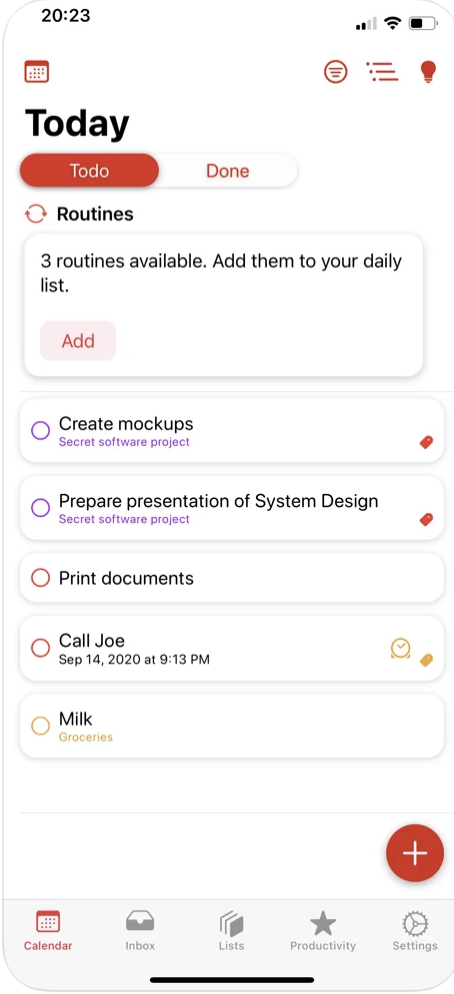
\includegraphics[width=4cm]{./graphics/planny4.png}
	\caption{An image of the 'today' view in the application Planny4\cite{reutter_2020}.}
	\label{fig:planny4}
	
\end{figure}
	        
	        There are many valuable features available in this application, the best one being the assistant suggesting ways to create a productive day.  However, apart from that, there are no other distinguishing features in this application that make it any better than other similar applications in the App Store.  The application also requires a subscription to unlock all features, and so is not an ideal solution for users unable to pay, such as students or low-income users.
	        
	        \subsection{24me - Smart Personal Assistant}
	        
	        24me\cite{24me} is an application available on iPhone, iPad and Apple Watch only and is mainly sold as a personal assistant more than a to-do or time management application.  Tasks can be viewed in a calendar (Figure~\ref{fig:24me}) or as a list, including reminders and labels.  The application also offers a way to automatically dial into conference calls, as well as Outlook email account integration and estimated times to get from one place to another.
	        
	        \begin{figure}[htb]

	\centering
	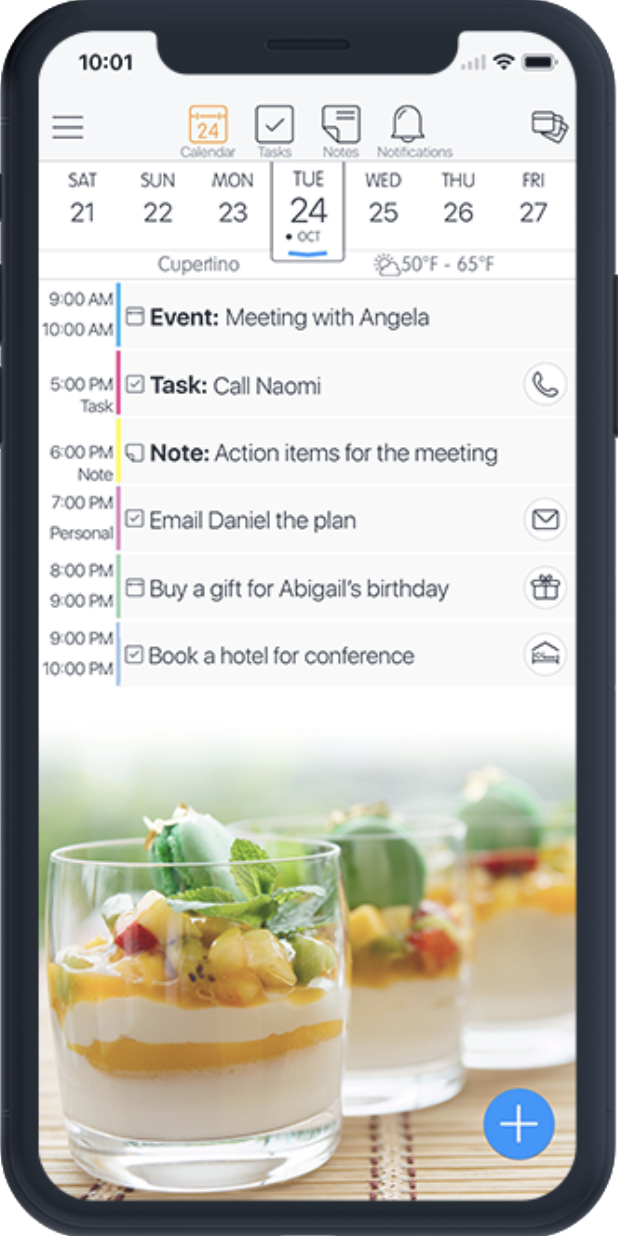
\includegraphics[width=4cm]{./graphics/24me.png}
	\caption{An image of the calendar view of the application 24me\cite{24me}.}
	\label{fig:24me}
	
\end{figure}
	        
	        This application has many unique features that are not seen in other productivity applications, such as conference calling and micro gifting, but the most basic features seem to need refinement.  Tasks cannot be customised much, and the UI, in general, seems to require some modernisation in order for this application to be a genuine competitor to other applications on the market.

	        \subsection{Any.do - Calendar and Reminders}
	        
	        Any.do\cite{any.do} is available on many different platforms, including Apple, Android, Windows and smart home devices.  The application allows users to create lists, view calendars, reminders and includes a daily planner.  Natural language processing is used to cherry-pick dates, times and location from reminders to make suggestions based on these items.  There are also extra features available on the premium version, including recurring, WhatsApp and location reminders, tags, themes and an unlimited daily planner.
	        
	        \begin{figure}[htb]

	\centering
	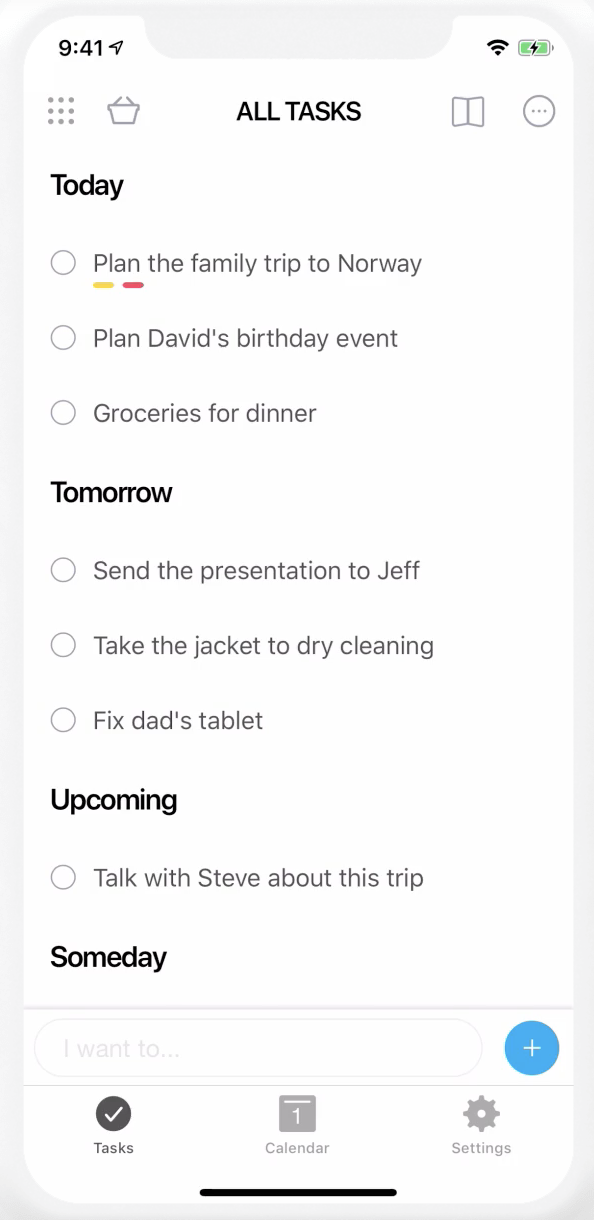
\includegraphics[width=4cm]{./graphics/anydo.png}
	\caption{An image of the task list view in the application any.do\cite{any.do}.}
	\label{fig:anydo}
	
\end{figure}
	        
	        Although this application does not necessarily boast any particularly unique features, the way the features have been implemented is elegant, making the application seem enjoyable to use and not too time-consuming for the user.  Tasks and reminders can be reordered easily, and the natural language processing features make creating new reminders a lot more efficient, which emphasises the purpose of the entire application.  However, it does seem incomplete without access to the premium features, which would be expected in a basic time management application, such as the tags and recurring reminders.
	        
	        \subsection{Things 3}
	        
	        Things 3\cite{things_3} is a paid application that allows users to create 'areas' to represent different parts of their life.  Within the 'areas', the user can create projects and plans that include to-do items and reminders, calendar integration, tags, and 'quick find'.  The application is available on all Apple platforms and synchronises all user data between these devices if the user is signed in on more than one device.
	        
	        \begin{figure}[htb]

	\centering
	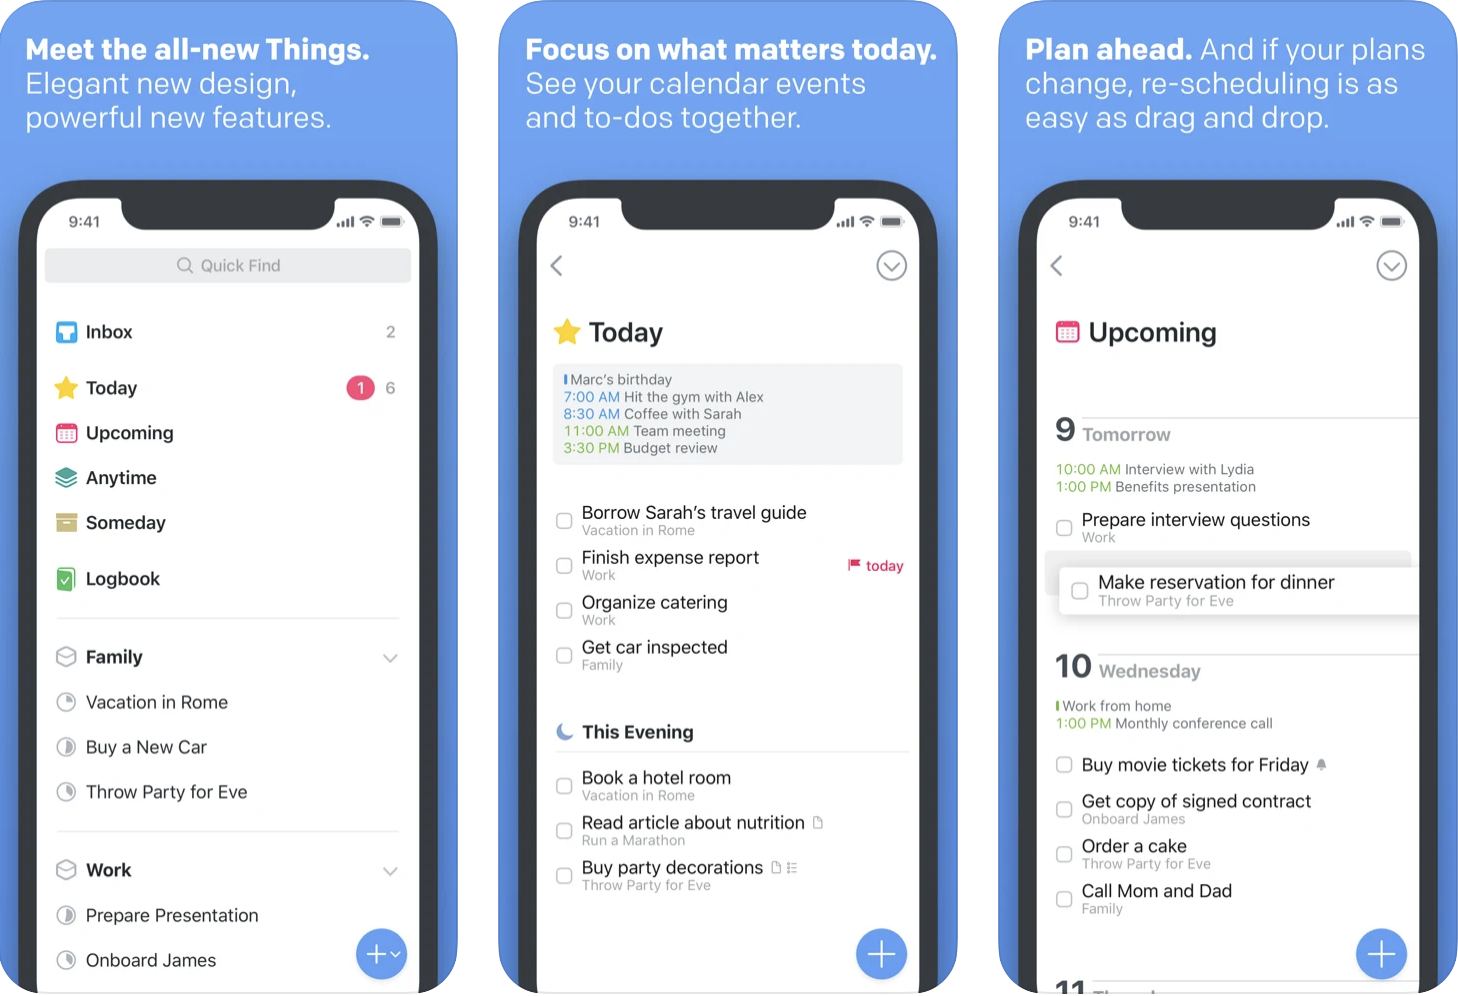
\includegraphics[width=10cm]{./graphics/things3.png}
	\caption{An image showing 'areas', today and this evening tasks and upcoming tasks in the application Things 3\cite{things_3}.}
	\label{fig:things3}
	
\end{figure}
	        
	        The main selling point for this application is that it allows the user to manage their time very precisely and do this for multiple areas of their life.  The 'areas' feature completely separates a users' career from their personal life for example.  Because of this, it is quite a strong competitor in the productivity application market.  The downside of this application is that the user must pay to download it; there is no free version or trial for the application to be tested, which can deter users from even trying the application. However, this can also be viewed positively. A subscription is not required to use the application. It is just a one-off payment, so if the user intends to use the application in the long term, it may be a worthwhile investment.
	        
	        \subsection{Sorted3}
	        
	        Sorted3\cite{sorted} is an application designed for 'hyper-scheduling' a users day.  It does this by putting all user events and tasks into a single unified timeline, so an entire day's outlook can be displayed.  The user can also tap on an event or task and add more detailed notes within the item to be referred back to if needed.  These notes can include a to-do list, tags and reminders for extra flexibility.  Features also include a timeline view, 'magic selection' of items so multiple can be selected at once, as well as natural language processing and Siri integration.
	        
	        \begin{figure}[htb]

	\centering
	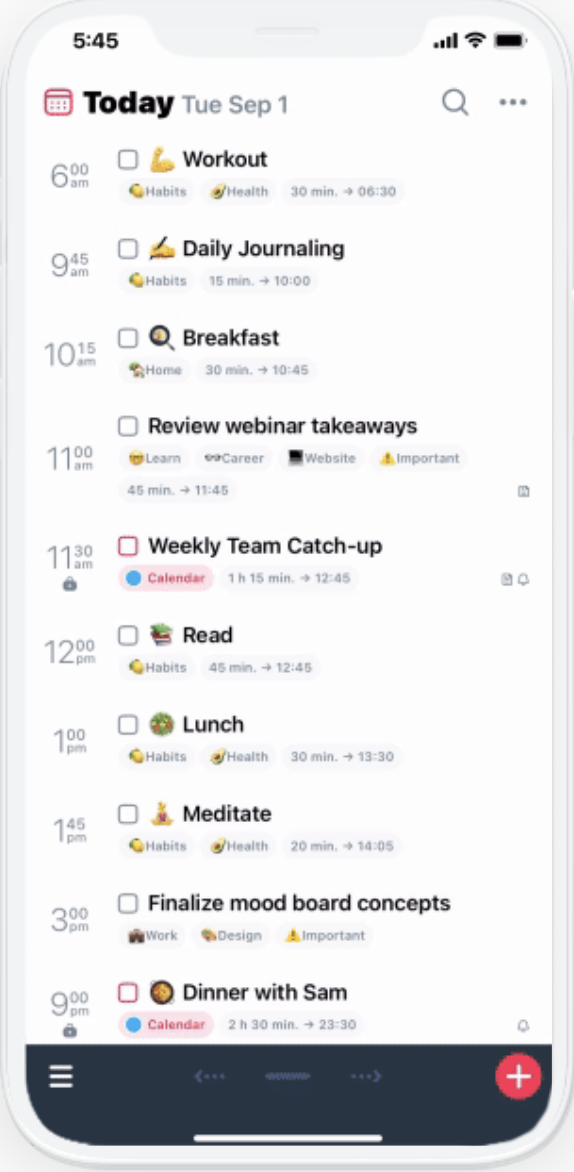
\includegraphics[width=4cm]{./graphics/sorted3.png}
	\caption{An image of the unified timeline feature withint the application Sorted3\cite{sorted}.}
	\label{fig:sorted3}
	
\end{figure}
	        
	        The most significant advantage of this application is that it gives users access to features expected to be part of the premium features.  For example, the unified timeline is quite a powerful feature considering it allows the user to view a complete overview of their day and add extreme detail to the items in the timeline if needed.  It also stands out from its competitors with features such as the 'magic selection' tool and the time ruler and calendar drawer.  There does not seem to be any other applications that offer these specific features, making Sorted 3 seem a much more elegant and well thought out choice.  As with many other applications, there are features only available with the premium option, including auto-scheduling and adding attachments to items.  However, the premium option is on a pay-once basis and offers features that are not necessarily considered compulsory for a productivity application.
	        
	        \subsection{OmniFocus 3}
	        
	        OmniFocus 3\cite{OmniFocus} is an application based on task management that users can use to create projects and add actions to them.  Various tags can be added to actions such as location, energy level and priority.  The perspectives view can help the user plan their day by seeing the subsequent actions that need to be completed.  A pro version allows the user to view a custom home screen and sidebar, a forecast tag, and custom perspectives.  This application is only available on Apple platforms or as a web application.
	        
	        \begin{figure}[htb]

	\centering
	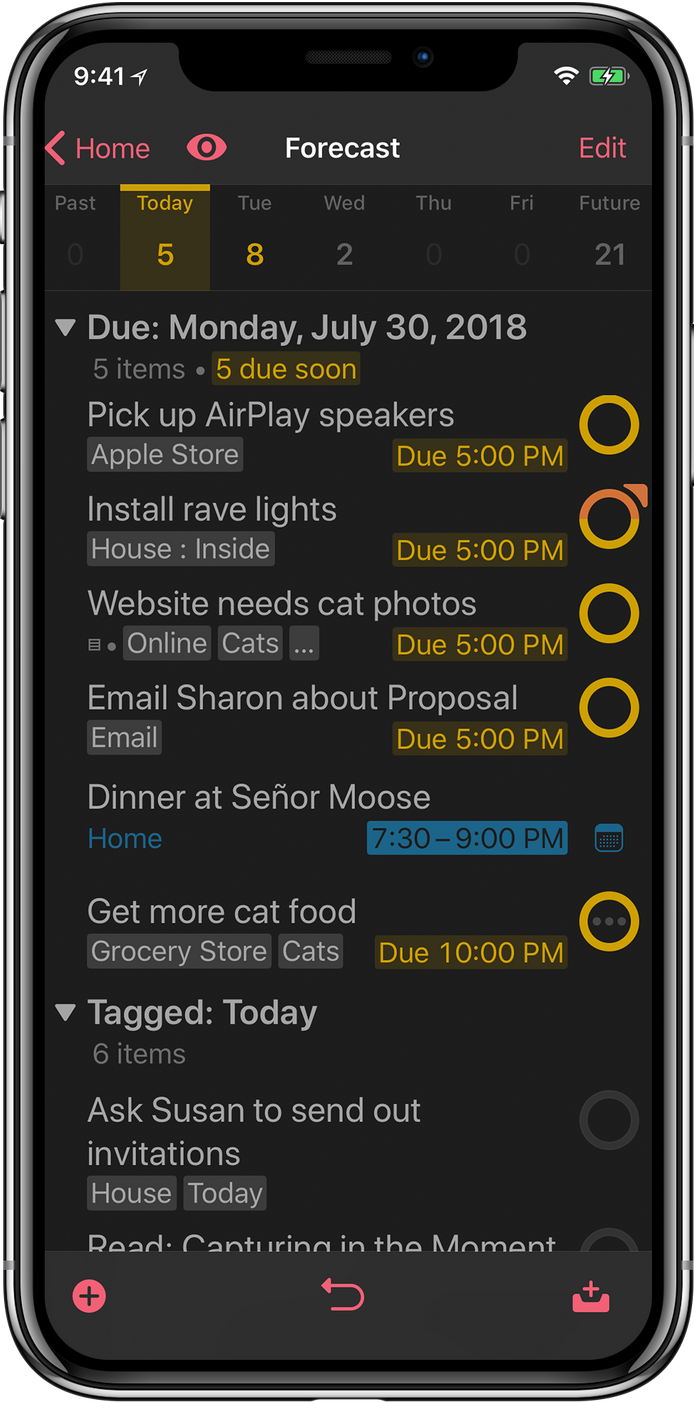
\includegraphics[width=4cm]{./graphics/omnifocus3.png}
	\caption{An image of the custom forecast tag within the pro version of the application Omnifocus\cite{OmniFocus}.}
	\label{fig:omnifocus3}
	
\end{figure}
	        
	        This application has many useful features but no features that particularly stand out against the other task management applications on the market.  The flexible tag management makes organising and batching actions a more intuitive process, and the perspectives view is also an excellent tool to allow the user the manage their time.  The features offered at a premium for the application are limited, especially as the price for premium access seems to be higher than the average. However, the user is offered two ways to pay for premium; a one-off payment that gives access to the iOS application only or a subscription that gives access to all platforms.
	        
	        \subsection{Related Work Summary}
	        
	        After taking into account the features available on various pre-existing productivity applications, it has been determined that the following features are considered indispensable for this application:
	        \begin{itemize}[noitemsep]
	            \item Creation of tasks, events and reminders.
	            \item Auto-scheduling.
	            \item Completely free access to the application.
	        \end{itemize}
	        
	        As discussed later in the document, Agendum has provided these features and other features which are highlighted in the requirements analysis.

\chapter{Legal, Professional, Social and Ethical Issues}
	\label{chap:legal_social_ethical_issues}
	In this chapter, the issues that could have arisen during the project will be discussed.  In Section~\ref{sec:issues_legal}, the legal issues that a mobile application developer must consider will be explored, and then in Sections~\ref{sec:issues_professional} and~\ref{sec:issues_ethical}, the social, ethical and professional considerations will be discussed.
	
	\section{Legal Issues}
	    \label{sec:issues_legal}
	    \subsection{General Data Protection Regulation}
	    When developing software that handles any personal data it must comply with the principles defined in the General Data Protection Regulation (GDPR) or similar laws in other countries.  The key principles defined in the GDPR are as follows:
	    \begin{itemize}[noitemsep]
	        \item Lawfulness, fairness and transparency.
	        \item Purpose Limitation.
	        \item Data minimisation.
	        \item Accuracy.
	        \item Storage Limitation.
	        \item Integrity and confidentiality.
	        \item Accountability.
	    \end{itemize}
	    \cite{ico_principles}
	    
	    The basic definition of these principles is that the personal data stored by companies should only be used for the purpose they have been specified, excessive data should not be stored, the data should be stored safely, and the reason the data is being stored should be transparent to the consumer.  If the software fails to comply with these principles, the software developer(s) responsible and/or the company can face lawful action.
	    
	    In this projects' context, these principles were kept in mind, and an effort has been made to ensure only the data needed for the application is stored.  The personal data used in the application includes email and bio-metrics (for biometric authentication).  The purpose of the email address is to give a user a unique account which can then be used to log in and connect with other users.  Biometric authentication is entirely optional and asks the users' permission before being activated.  The user is also presented with a message as to why they may want to activate the biometric authentication.  Email is stored in Firebase, which has its own security, as well as the access rules that were implemented manually when the database was set up.  The storage of biometric data is handled by the iOS operating system and is stored in the Apple Keychain associated with the Apple account logged into the iPhone.  With all of the above in place, it can be assumed that the application complies with the GDPR.
	    
	    \subsection{Intellectual Property Rights}
	    Another legal aspect of software engineering is whether to apply for intellectual property rights.  Having intellectual property protection means that other companies cannot steal or copy a recognised products' designs or implementation without facing legal action.  Types of intellectual property rights include copyright, patenting and trademarks\cite{intellectual_property}.
	    
	    Applying for intellectual property rights was never considered for this project as the application had a limited purpose of only being used for a university project.  However, if the application were to  be put on the App Store, having intellectual property rights would  be considered.
	    
	\section{Professional Issues}
	    \label{sec:issues_professional}
	    
	    \subsection{British Computer Society Code of Conduct}
	    There are many different codes of conduct from various professional bodies that can be followed when developing software.  These codes of conduct are not required by law but can make the software more accessible and within the public interest.  In this section, the code of conduct provided by the British Computer Society will be discussed.  The BCS code of conduct is comprised of four main principles:
	    \begin{itemize}[noitemsep]
	        \item You make IT for everyone.
	        \item Show what you know, learn what you don't.
	        \item Respect the individual or organisation you work for.
	        \item Keep IT real. Keep IT professional. Pass IT on.
	    \end{itemize}
	    \cite{bcs}
	   
	   These principles ensure that everyone is treated equally. No one claims they have a competency level that they do not have and every software engineer claims responsibility for their work. They uphold their reputation, as well as the reputation of BCS.
	   
	   Although these principles were not considered from the beginning of the project, they have been upheld throughout.  Any third party that has been interacted with during the project has been treated equally, and everyone involved in the project has taken responsibility for their work.
	    
	\section{Social and Ethical Issues}
	    \label{sec:issues_ethical}
	    
	    \subsection{Privacy}
	    A popular topic regularly covered in the technology realm is privacy, particularly user privacy.  Apart from personal data, which is protected by law, the ethics of how non-personal data should be stored tends to be a grey area.  In the context of the application, an attempt has been made to ensure the least amount of data possible is stored. If it is stored, it is done securely in a Firebase database and requires user authentication to be accessed.  All data apart from the unique user ID's can be seen and downloaded by the user within the application, so there is no 'secret' data being withheld from the user.
	    
	    \subsection{Price}
	    Another topic that is debatable in terms of ethics is the price software should cost.  Many applications and services now offer a subscription-based payment system rather than a one-off payment system. Even though this is an excellent way to ensure the software is maintained, it also generates more profit for the company.  When determining whether there should be a cost for the application produced in this project, the target market was the primary consideration.  The application is designed to be used by anyone who wants to be more deliberate with managing their time, but the fact that students, in general, do not seem to have a suitable free-to-use application was the inspiration for this project.  Therefore, the decision was made to make the application completely free without advertisements to ensure it remains accessible to everyone, especially those who cannot afford to pay for an application of this type.

\chapter{Software Development Life Cycle}
	\label{chap:sdl}
	This chapter will discuss the model initially chosen for this project and reflect on whether it was the most suitable choice or whether it would have been better if a different model was chosen.  This chapter will also cover the risk analysis for the project.
	
    \section{Software Development Model}
        \label{sec:sdl_model_chosen}
        The model chosen for this project was a slightly altered scrum agile approach.  The traditional method includes having a team with a scrum master who assigns tasks to each team member.  All tasks are created before the project begins and put into the backlog, and then every 2-4 weeks, there is a sprint review to add or move tasks, ensure no issues have arisen, and make sure all team members are still on task\cite{sommerville_2018}.
        
        \begin{figure}[H]

	\centering
	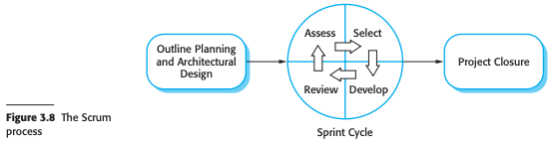
\includegraphics[width=8cm]{./graphics/scrum.png}
	\caption{A diagram of the scrum methodology	\cite{sommerville_2018}.}
	\label{fig:scrum}
	
\end{figure}
        
        The inspiration for this methodology was that an agile approach is widely used in industry and would be the most realistic for a project of this nature.  As only one person developed the application, the regular stand-up meetings and sprint reviews could not occur in the usual way.  A sprint review still took place at the end of every sprint, but no stand-up took place.  To keep track of tasks in the backlog and the current sprint, Trello was used, along with a third-party extension called TeamGantt.
        
        \begin{figure}[H]

	\centering
	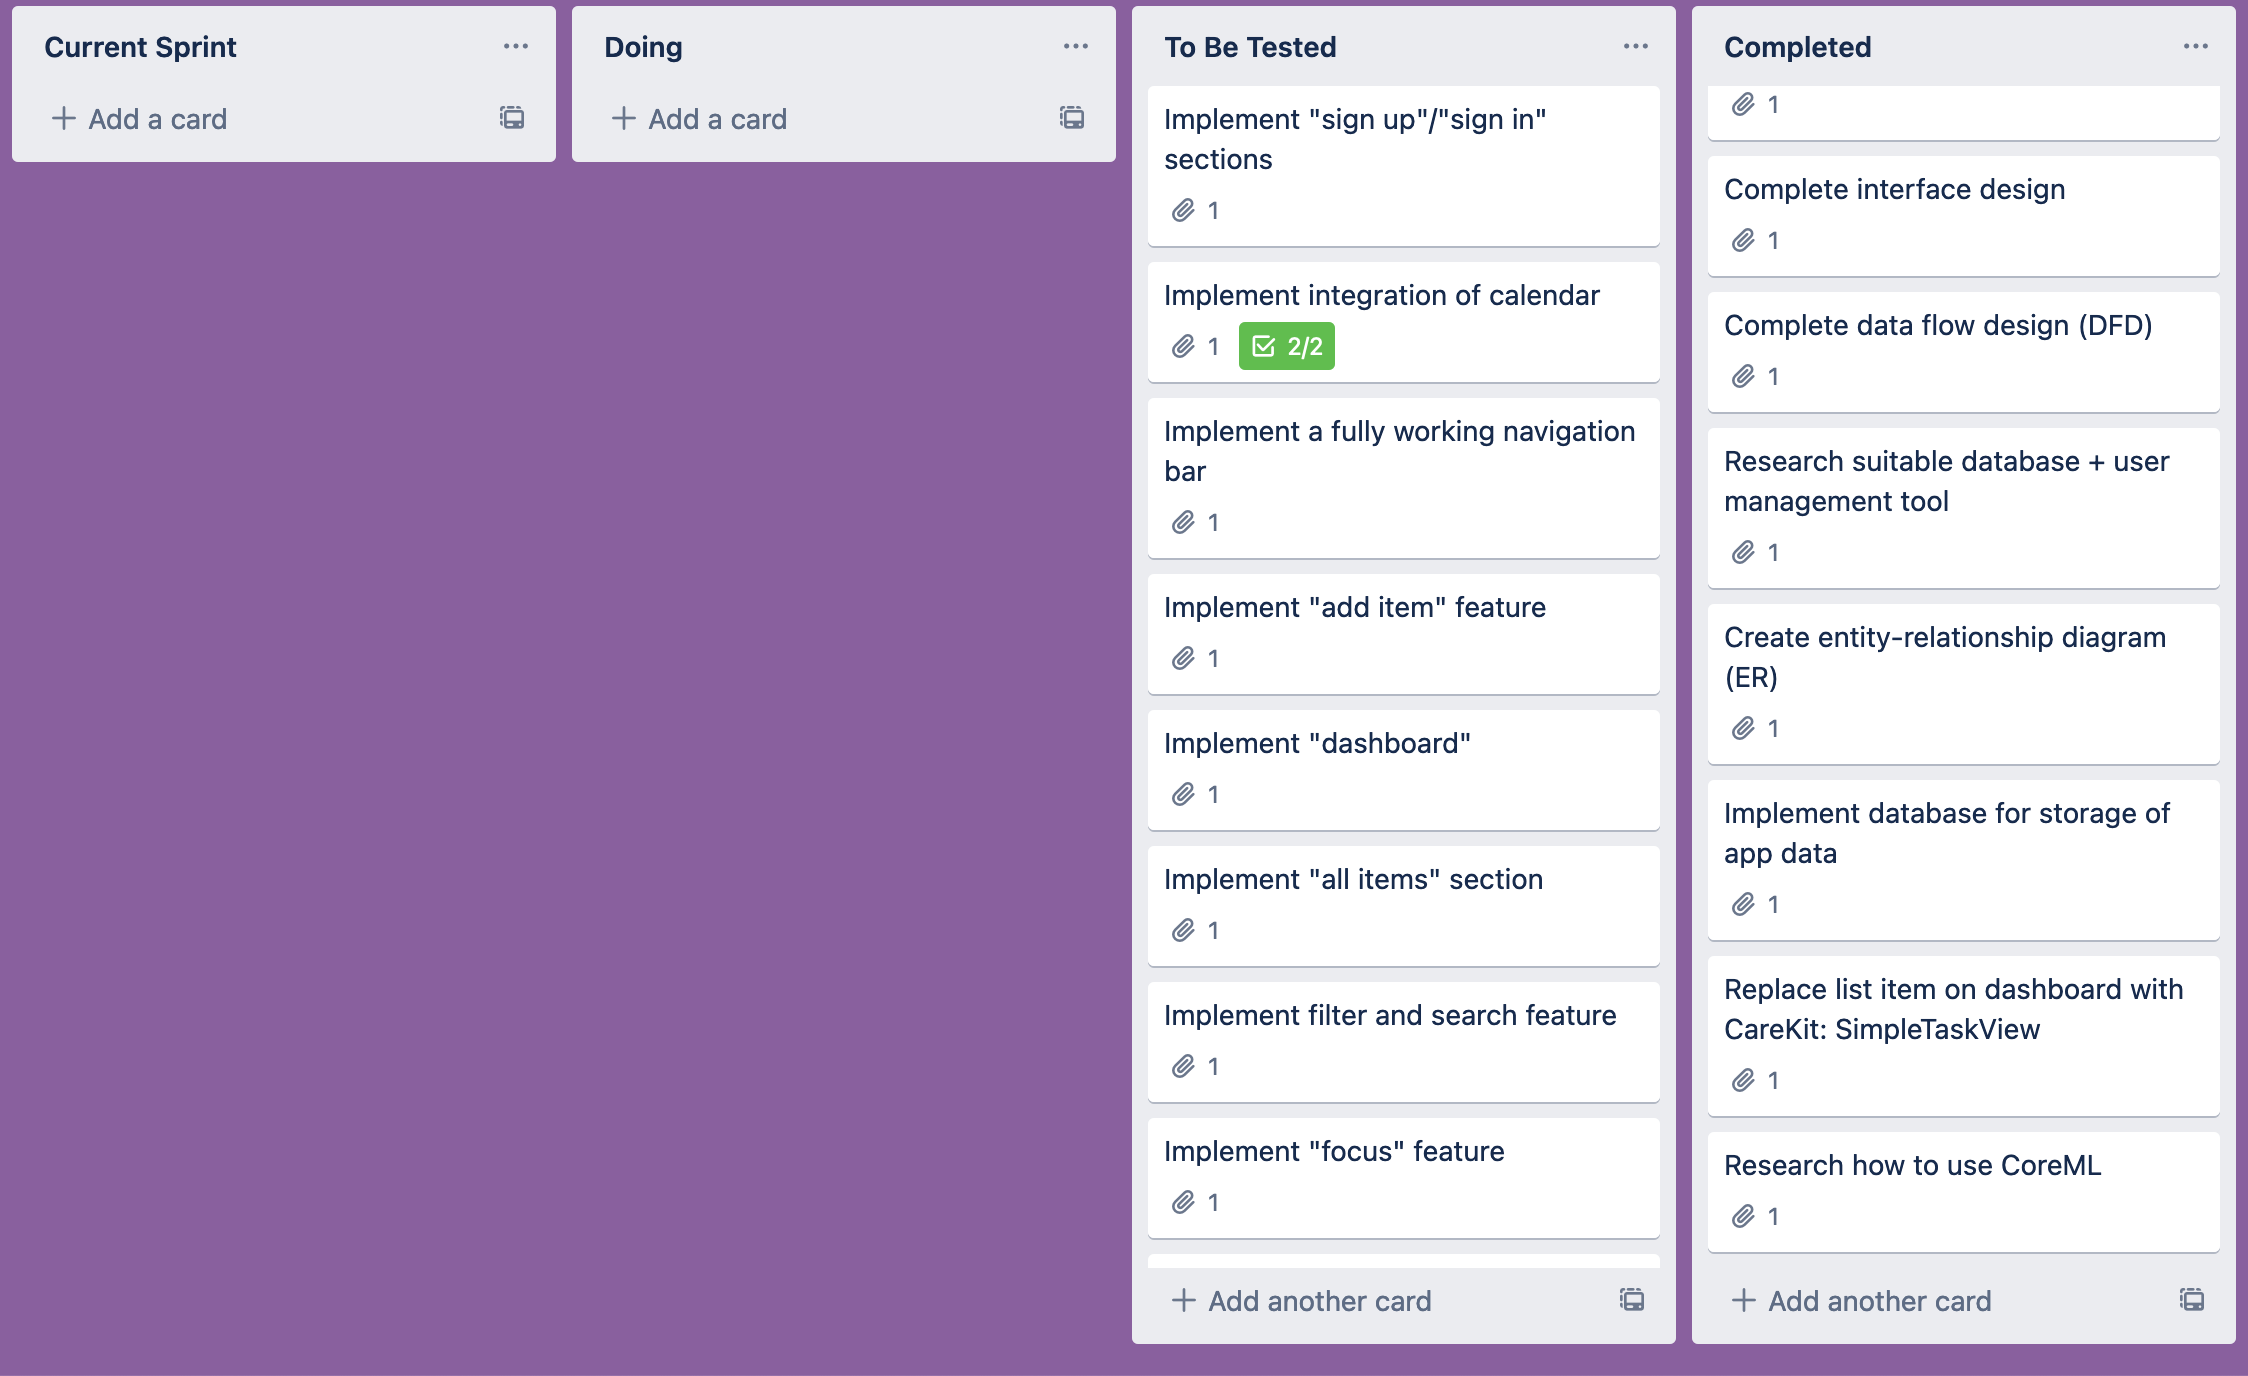
\includegraphics[width=12cm]{./graphics/trello.png}
	\caption{An image of Trello with completed tasks.}
	\label{fig:trello}
	
\end{figure}
        
        After using this model for the project, it seems to have remained the most suitable choice.  The regular sprint reviews ensured that the project stayed on track and completed tasks on time.  However, the prediction of upcoming tasks created before beginning the application could have been improved.  While implementing the application, it became clear some tasks that had not been anticipated were missing. These needed to be added in, resulting in the expected time frame of project completion being affected.  Overall, this did not affect the project's outcome, and the application mainly was completed on time apart from the testing phase (which will be discussed later in this document).
        
        For reference, the Gantt chart created before starting the application implementation has been placed in the appendix.
        
    \section{Risk analysis}
        \label{sec:sdl_risks}
        At the beginning of the project, potential risks had been defined and scored based on the likelihood and impact they would have on the project\cite{intial_document_pike} - Table~\ref{app::risk_table} in the appendix details these risks and their mitigation definitions.
        
        In Chapter~\ref{sec:reflection_risk}, a reflection of the risks specified at the beginning of the project will be discussed and any unforeseen risks that arose during the project and how they were dealt with.


\chapter{Deliverables}
    \label{chap:deliverables}
    This chapter will present the deliverables produced during the project in the order of the stages defined in the software development model.  Section~\ref{sec:deliverables_requirements} will cover the requirements analysis, Section~\ref{sec:deliverables_design} will contain the design documentation, Section~\ref{sec:deliverables_implementation} will discuss the implementation, and finally, Section~\ref{sec:deliverables_testing} will contain the testing documentation.
    
    \section{Description of project}
        \label{sec:deliverables_description}
        This project produces an application available on the iOS platform only, with the potential to be expanded to other platforms such as iPadOS, WatchOS and Android; however, those platforms remain outside of this projects scope.  The application is built using the Swift programming language, and Firebase handles the interaction between the application and the Google servers.  The UI for the application is built using SwiftUI and UIKit.
        
    \section{Requirements Analysis}
        \label{sec:deliverables_requirements}
        The project requirements were based partly on what is seen as the basic features expected in a productivity and time-management application and partly on the results of the questionnaire that was sent to prospective users (Appendix~\ref{app::questionnaire}). This questionnaire collected data on the current employment status of the potential user and what feature would make them want to download and use a productivity application.  The questionnaire also asked the prospective users their thoughts on a task suggestion feature and whether they would utilise such a feature and why.
        
        Following this, a list of requirements was generated at the start of the project; however, it was expected that these requirements could change based on the obstacles reached during development.  Therefore, the revised set of requirements, split into functional and non-functional, has been defined and can be found in Table~\ref{app::requirements_table}.
        
        Compared to the requirements defined at the start of the project, some requirements have been removed, and some requirements were defined as "time-permitting"; these were not completed.  The removed requirements included seeing a friend's recent activity within the application. This was removed because the infrastructure needed to implement this requirement was not available.  The requirements also defined the use of a tutorial when the user was first to use the application, however, this requirement was also removed due to the application being self-explanatory.  The non-compulsory requirements included adding items using Siri (the virtual assistant available on Apple devices) and being able to add and complete items displayed in a 'Widget', which was a new feature provided by Apple when iOS 14 was released in 2020.  Due to time constraints, neither of these requirements were included.
        
    \section{Design}
        \label{sec:deliverables_design}
        In the sections below, the designs produced for the project will be presented and discussed.  The designs will include the UI design (Section~\ref{subsec:UI_design}), Data flow design (Section~\ref{subsec:DFD}), entity relationship design (Section~\ref{subsec:E-R_diagram}) as well as testing design (Section~\ref{subsec:test_design}).  Each section will include a short reflection, including whether the designs were met in the implementation and whether any changes were made.
        
        \subsection{User Interface Design}
        \label{subsec:UI_design}
        For the UI design, wireframe designs were first created to get an idea of how the application should generally look without deciding on colours and fonts.  These wireframes were created using Balsamiq Mockups 3 and can be viewed in Section~\ref{app::mockups} of the appendix.  The application is designed to have a minimalist type theme, so an attempt was made to ensure the UI was self-explanatory and straightforward in terms of features.  There is a navigation bar placed at the bottom of the application, which remains consistent throughout all the views to ensure the application's navigation is easy. Every screen is only one tap away.
        
        In Section~\ref{app:colour} of the appendix, the coloured designs based on the wireframe mock-ups can be found.  At this point in the design process, a colour scheme had been chosen (Figure~\ref{fig:colour_scheme}) and the font scheme and the icons provider.  The font scheme chosen was the Montserrat family, and the icons would be sourced from the site icons8 as they had free icons that could be used in the application.
        
        \begin{figure}[H]

	\centering
	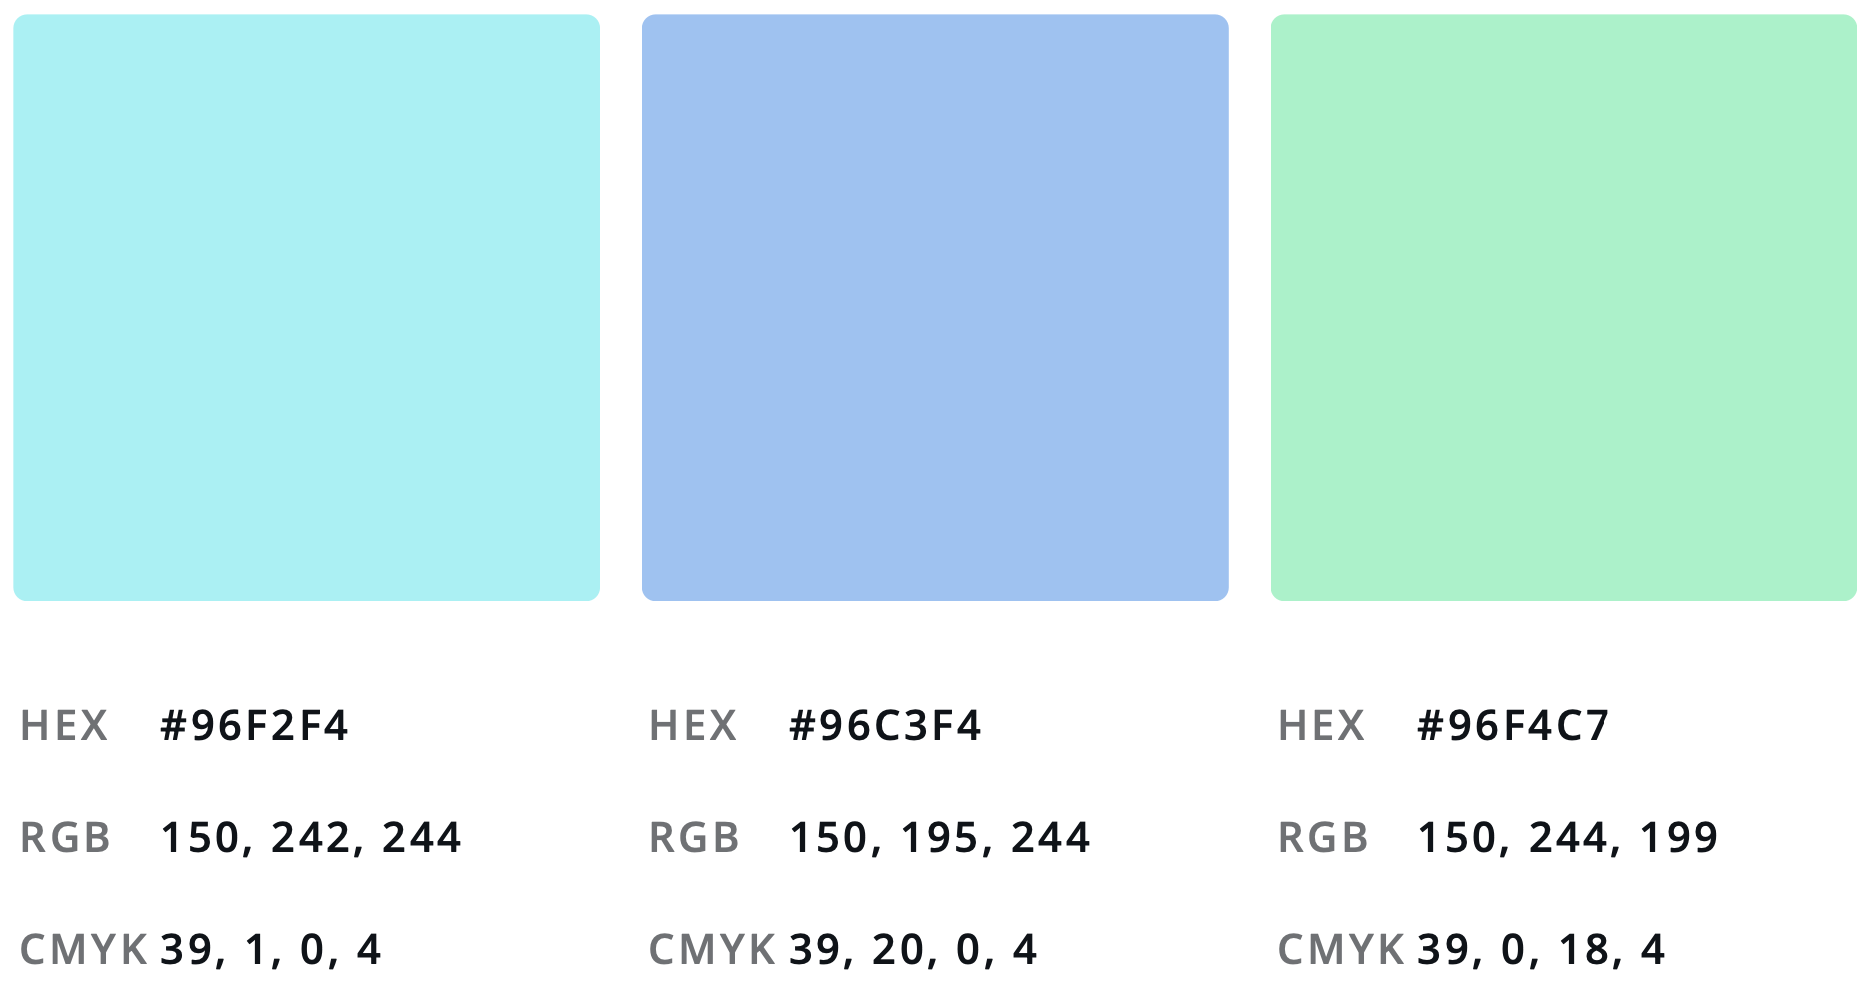
\includegraphics[width=4cm]{./graphics/design/Colours.png}
	\caption{The colour scheme used in the application.}
	\label{fig:colour_scheme}
	
\end{figure}
        
        Overall, the application was mainly able to imitate the designs produced. However, some changes did need to be made.  An attempt was made to use the Montserrat font family in the application. However, XCode did not seem to support this, and the application would render with the default system font usually provided with iOS applications.  The streak statistics initially shown in the wire-frames were not continued into the coloured design or the application because this feature was unable to be provided due to limitations with the SwiftUI framework. The design also showed suggestions as events in the calendar view. However, this was not possible during implementation due to limitations with the third-party library used, so suggestions are now only made in the agenda view.  The designs contained a recent activity screen that could be navigated to from the 'friends' screen.  The recent activity view was still a feature in the final application but does not show a friend's recent activity.  It became apparent later in the implementation phase that this feature was not accounted for when designing the database. So it was not possible to add it into the application without significantly affecting the completion deadline, however, in future this feature could be added to the application.
        
        \subsection{Data Flow Diagrams}
        \label{subsec:DFD}
        Section~\ref{app:dfd} of the appendix shows the data flow diagrams generated during the project's design phase.  These diagrams show the flow of data between the user, the application and the database.  
        
        Figure~\ref{fig:signin_signup_dfd} shows the data flow for the sign in and sign up views.  The user inputs their login data into either the sign in or sign up view.  The sign in view will authenticate the user with the database, and the database will either return an authentication error or successfully authenticate the user.  The sign-up view will add the user to the database, and the database will either return with an error saying the user already exists or will successfully add the new user.
        
        Figure~\ref{fig:dashboard_allitems_dfd} shows the data flow between the dashboard and the all items view. The user will input item data into the add item view.  They then have the option to save the item to the database or cancel the action.  Cancelling the action will take the user back to the dashboard or the all items view, depending on which view the user accessed the add item view from. If the user saves the item, it will be saved to the database, and then the application will automatically navigate back to the dashboard or the all items view.  Both the dashboard and the all items view will then request a list of all items saved to the users' account from the database, and this list will then be displayed.
        
        Figure~\ref{fig:focus_dfd} shows the data flow for the focus view.  The user will input timer data when amending the focus timer settings, and these settings will then be passed to the main focus view.  These settings will be saved locally on the device.
        
        Figure~\ref{fig:friends_dfd} shows the data flow for the 'friends' view.  The user will input the user email they wish to add into the add friend view, and this will be sent to the database to search to see if the email exists.  If the email exists, the relevant data from that user account will be sent to the main 'friends' view.  When the 'friends' view is brought to the foreground of the application, it will request a list of all the user accounts the current user is associated with, and these user accounts will be passed to the view by the database.
        
        The data flow in these diagrams seemed to remain accurate during the implementation and would look very similar if they were reproduced again with the application already built.  However, they may have been more helpful if they were slightly more accurate; the database could have been specified more specifically. The application communicates with a user database that contains email and passwords only, and then another database containing item data associated with a user ID.
        
        \subsection{Entity-Relationship Diagrams}
        \label{subsec:E-R_diagram}
        Section~\ref{app:er} of the appendix shows the entity-relationship diagram produced during the design phase of the project.  The diagram shows the different objects stored in the database and the relation they have to each other and the user object.
        
        The user object is shown as having an email, password, and username, with the email and username making the primary key.  The event object is shown as having an ID, name, date, time and labels, with the ID being the primary key.  The reminders object is shown as having the same attributes as the event object.  The task object is shown as having the same as the reminder and event object, but with a habit element added.  One user can create one or more of an event, reminder or task. One reminder can have one event.  One reminder can have one task.
        
        Due to the ambiguity of how the database would work at the beginning of the project, this entity relationship diagram is no longer an accurate representation of how the various entities within the application are linked.  There are still events, reminders and tasks, and these can be generated as separate objects. However, all of them are derived from the same object named 'Item'.  Also, the user object was created without a username and has a unique ID generated by Firebase, which cannot be seen in the diagram.  The elements connected to the event, reminder and task entities are accurate.  An Item object contains all of these elements, so that is the only part of the diagram that remained consistent with the application.
        
        \subsection{Test Design}
        \label{subsec:test_design}
        The testing methods to be used during the project included UI testing, user testing and ad-hoc testing.
        
        For UI testing, it was decided that a "record and replay" approach would be taken as this was a feature already available in XCode and could mostly be automated.  This approach involves recording various interactions with the UI and then the IDE repeating these interactions during a test.  If the desired result is achieved, the test passes.  As a result, the "record and replay" tests were not included in the test design as it was unclear in many cases how exactly the application would behave in response to UI interaction.
        
        Ad-hoc testing involves using the application without any reference to a specific test case or plan\cite{software_testing}. This method was chosen because it was decided this was the quickest way to test the application as it does not require a test suite, therefore making the testing design time frame minimal. Testing could be mostly completed during the implementation phase.
        \vspace{\baselineskip}
        
    \section{Implementation}
    \label{sec:deliverables_implementation}
        In this section, the implementation of the application will be discussed. This will include talking through how the front-end was developed and an examination of the back-end, with code snippets and screenshots of the UI results available in the appendix.
        
        \subsection{Splash/Sign Up/Sign In}
        \subsubsection{Front-end}
        The splash screen was the only view in the entire application that used a storyboard file to create the view.  Storyboards are a feature native to UIKit but have been replaced with SwiftUI files with the introduction of the SwiftUI framework.  A storyboard was used for the splash screen because this was the default set up when a new project was created, and as the splash screen UI only contains a single label, it was felt that there was no need to change this.
        
        The UI for the sign-up and sign in views is very similar, with only the buttons' destination and the labels being slightly different. The sign-up view contains three text fields that allow the user to input a username, email and password. They can then click on the 'create account' button, which will validate their credentials and show the dashboard view (Figure~\ref{fig:splash_signup_signin_app}). If the user wishes to sign in with Facebook, they do not need to type in any credentials on the sign-up screen; they can tap the 'sign up with facebook' button, which will open a view taking them through the usual Facebook login. Images of the Facebook login process can be found at ~\ref{app:facebook_login_frontend} of the appendix.  After this is successful, the application will then navigate to the dashboard view. If the user taps on the 'sign in' button from the sign-up view, they will be taken to the sign-in view, where they can log in using their email and password or the Facebook login. Once again, successfully logging in will take them to the dashboard view.
        
        \begin{figure}[H]
    \centering
    \begin{subfigure}[b]{0.3\textwidth}
        \centering
        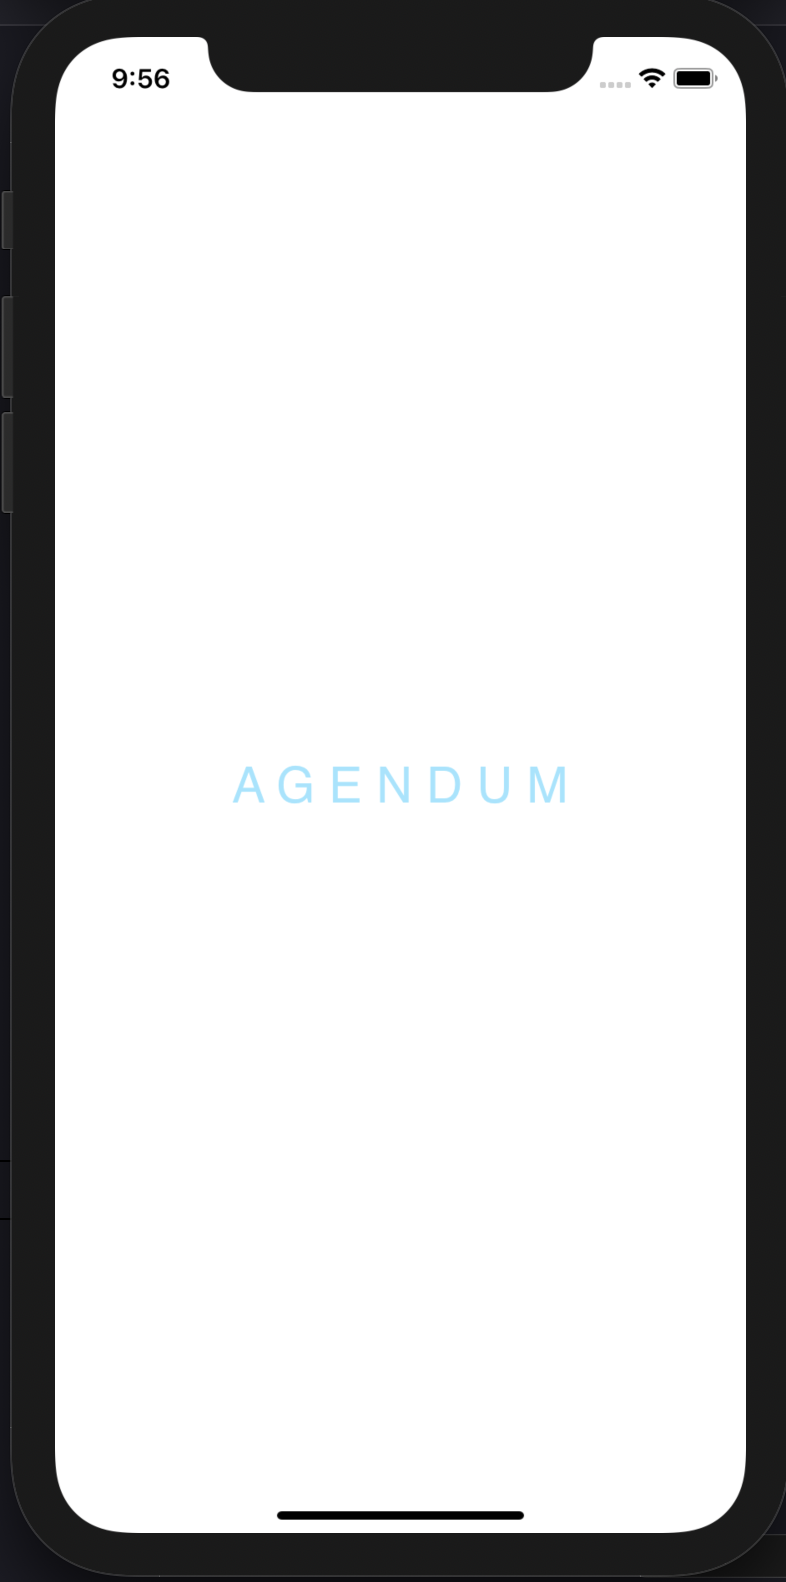
\includegraphics[width=\textwidth]{./graphics/Implementation/Splash_Sign_Up_Sign_In/splash.png}
        \caption{Splash Screen.}
        \label{fig:splash_app}
    \end{subfigure}
    \hfill
    \begin{subfigure}[b]{0.3\textwidth}
        \centering
        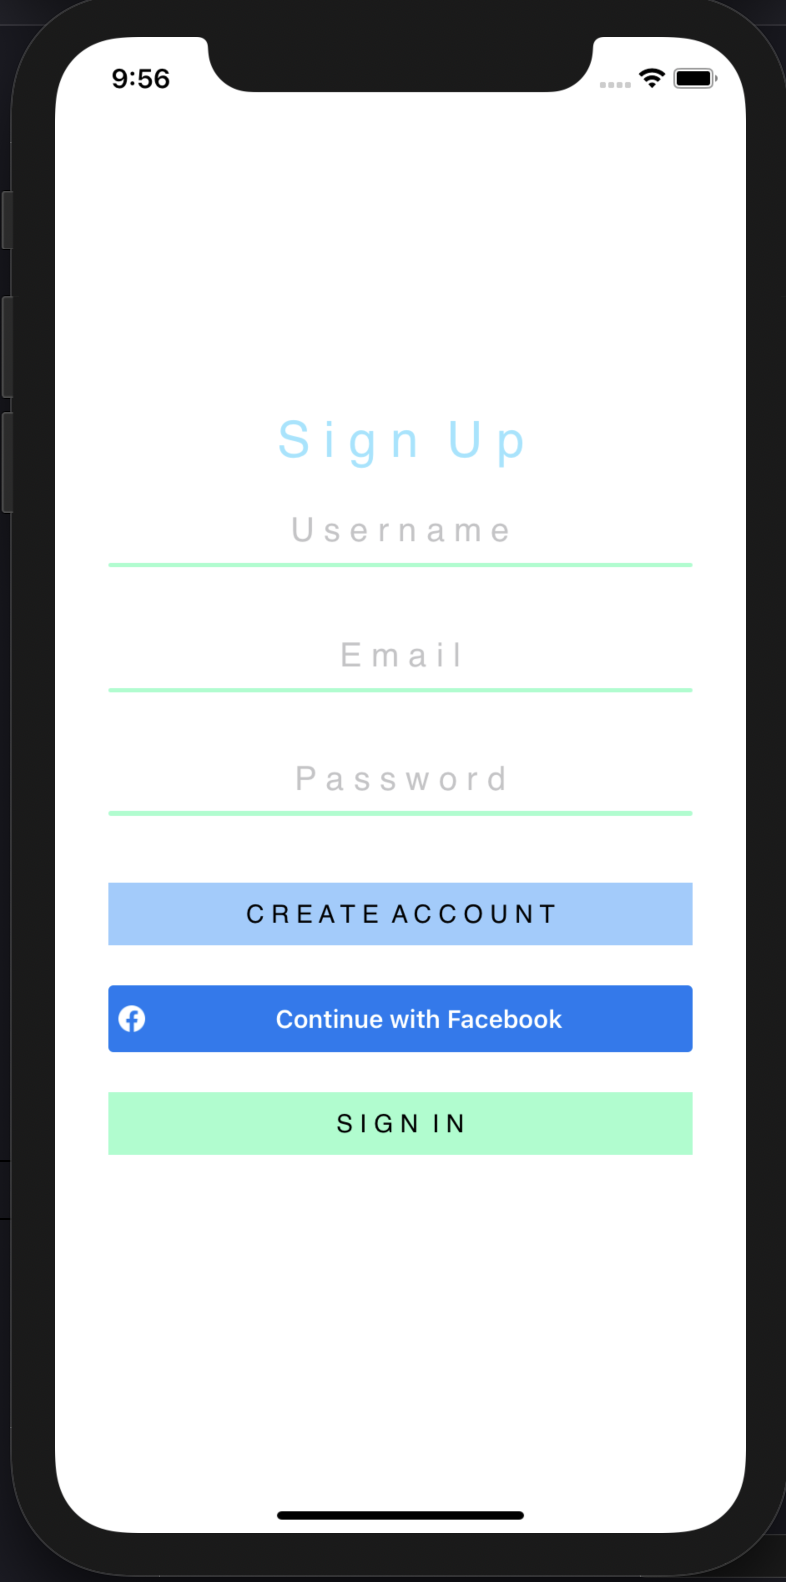
\includegraphics[width=\textwidth]{./graphics/Implementation/Splash_Sign_Up_Sign_In/signup.png}
        \caption{Sign Up.}
        \label{fig:sign_up_app}
    \end{subfigure}
    \hfill
    \begin{subfigure}[b]{0.3\textwidth}
        \centering
        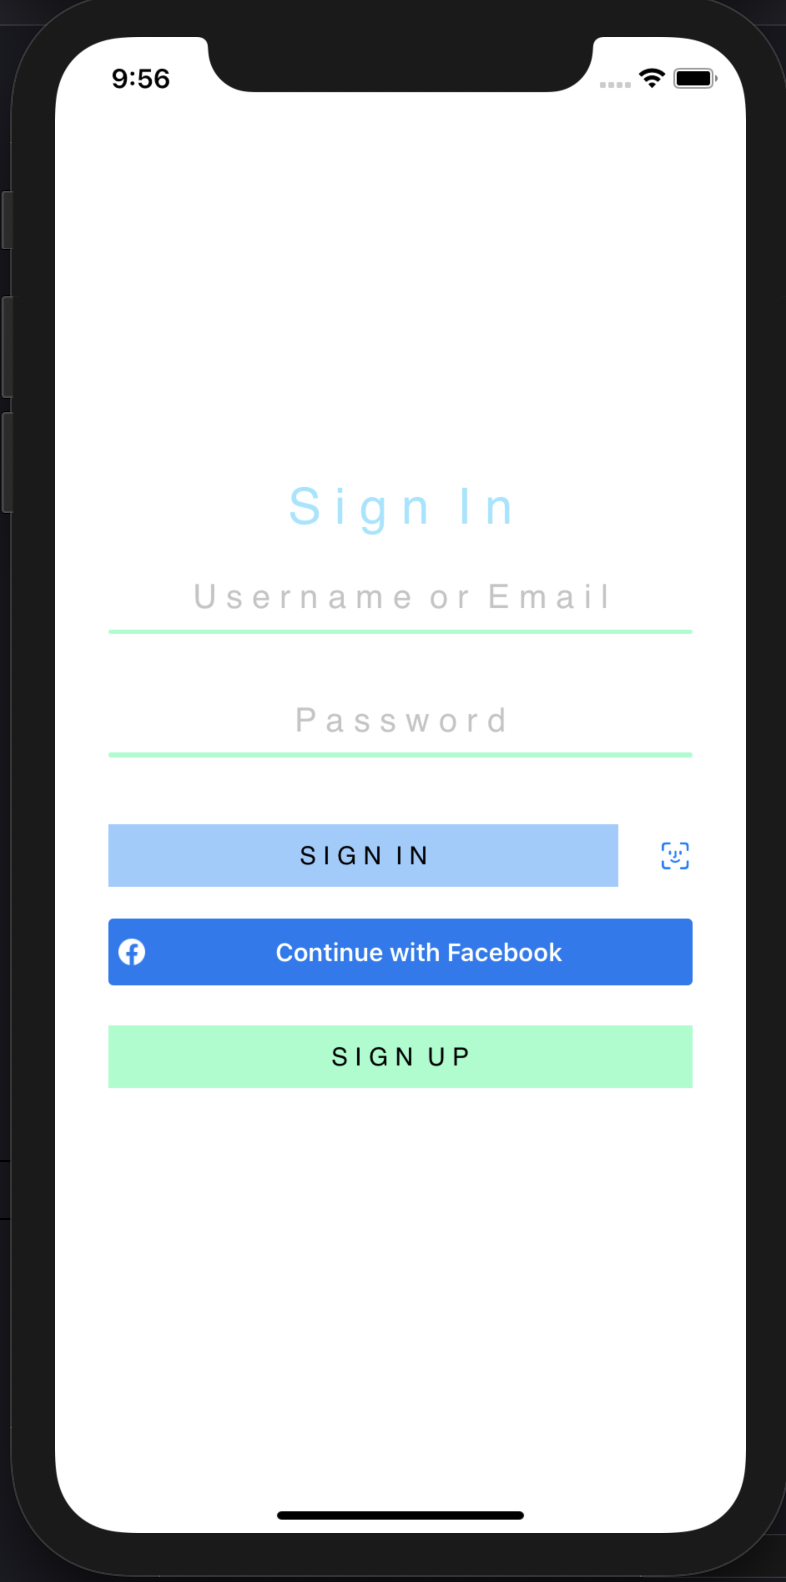
\includegraphics[width=\textwidth]{./graphics/Implementation/Splash_Sign_Up_Sign_In/signin.png}
        \caption{Sign In.}
        \label{fig:sign_in_app}
    \end{subfigure}
    
    \caption{Splash, sign up and sign in views shown in the application.}
    \label{fig:splash_signup_signin_app}
\end{figure}
        
        \subsubsection{Back-end}
        To officially register or log in a user, the application uses a class that communicates with the Firebase database using the Firebase API, installed using Cocoapods.  The code snippets for this class can be found in ~\ref{app:splash_signup_signin_backend} of the appendix.  The listen function is used to monitor authentication changes in the database.  If a change is detected, then the current logged in user is retrieved from Firebase, and the data returned is used to populate the User object within the application. The addUser function communicates with the Firestore database, populates the database with the user ID and adds an empty progress value.  This allows a user to add another user, as it is not possible to directly access the authenticated user database in Firebase for security reasons.  The addUsername function makes a call to the Firebase API to update a user profile and adds a username to that profile; however, during the development of the application, the use of usernames became obsolete as the user email is used to find other users and to primarily sign users in. The signIn and fbSignUp functions both make a call to the signIn function provided in the Firebase API but with slightly different parameters.  The regular sign-in uses email and password, but if Facebook sign-in is used, an AuthCredential object is passed as a parameter.  Finally, signUp makes a call to the createUser function provided in the Firebase API, and this uses email and password as parameters.  After this call is successful, the User object in the application is updated. The user password is stored in Apple Keychain to be used if bio-metrics is enabled in the application settings.
        
        When the user creates an account on the application, the storeGenericPasswordFor function will be called from the KeychainWrapper class.  This function simply stores the users' password in the relevant keychain directory and is secured by the iOS system.  When the user then attempts to sign in to the application with biometric authentication, the getGenericPasswordFor function will be called so that a password can be passed as a parameter to the signIn function contained in the FirebaseSession class.
        
        \subsection{Dashboard}
        \subsubsection{Front-end}
        The dashboard view contains many sub-views that handle the applications' primary purpose, which is to create and complete tasks.  All views in the dashboard will have to time frame at the top, the progress bar, and whether the view is in agenda or calendar mode.  The titles are custom elements made up of a Text object and a Horizontal Line object.  The progress bar is a Progress View object.
    
        The dashboard's default view is the agenda today view, which will show the items that need to be completed today in list form.  The items are split into events, reminders, tasks and suggestions, and are placed into these categories depending on the settings chosen when creating the item.  Each item is created from a Simple Task View, which is obtained from the CareKit module.  The view also contains an add button in the bottom right-hand corner, which will navigate the application to the add item view when tapped.  From this view, the user has a choice to swipe left on 'today' to switch to 'this week' or 'this month', or to swipe left on 'agenda' to switch to the calendar view for the corresponding time frame.  The swiping gesture is made possible because of the SwiftUIPager library, which allows the titles to be encapsulated in a Pager object.
        
        \begin{figure}[H]
    \centering
    \begin{subfigure}[b]{0.3\textwidth}
        \centering
        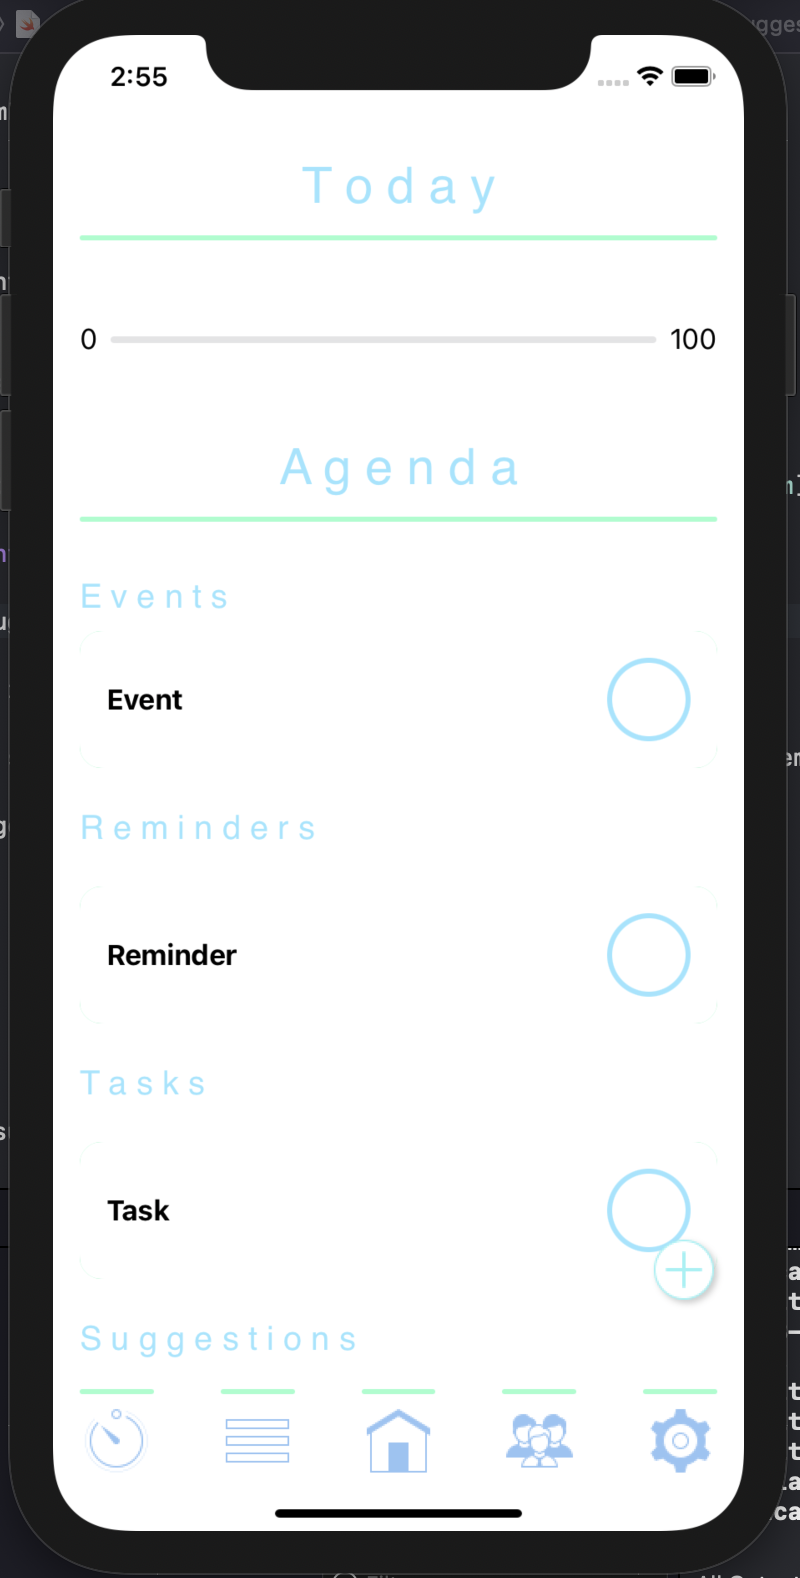
\includegraphics[width=\textwidth]{./graphics/Implementation/Dashboard/agenda today populated.png}
        \caption{Agenda Today.}
        \label{fig:agenda_today_app}
    \end{subfigure}
    \hfill
    \begin{subfigure}[b]{0.3\textwidth}
        \centering
        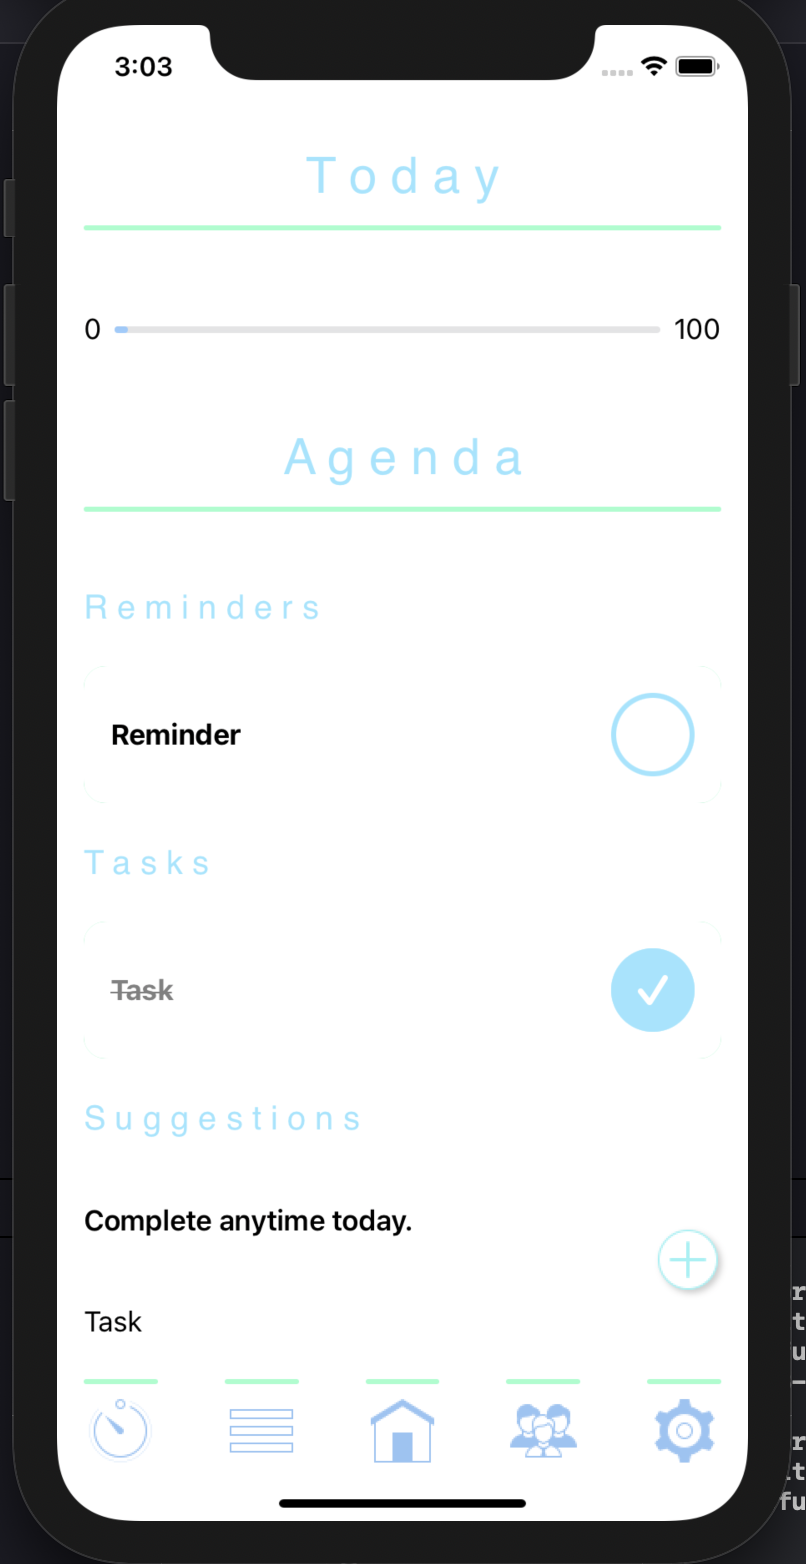
\includegraphics[width=\textwidth]{./graphics/Implementation/Dashboard/agenda today completed task.png}
        \caption{Task completed.}
        \label{fig:agenda_today_complete_app}
    \end{subfigure}
    \hfill
    \begin{subfigure}[b]{0.3\textwidth}
        \centering
        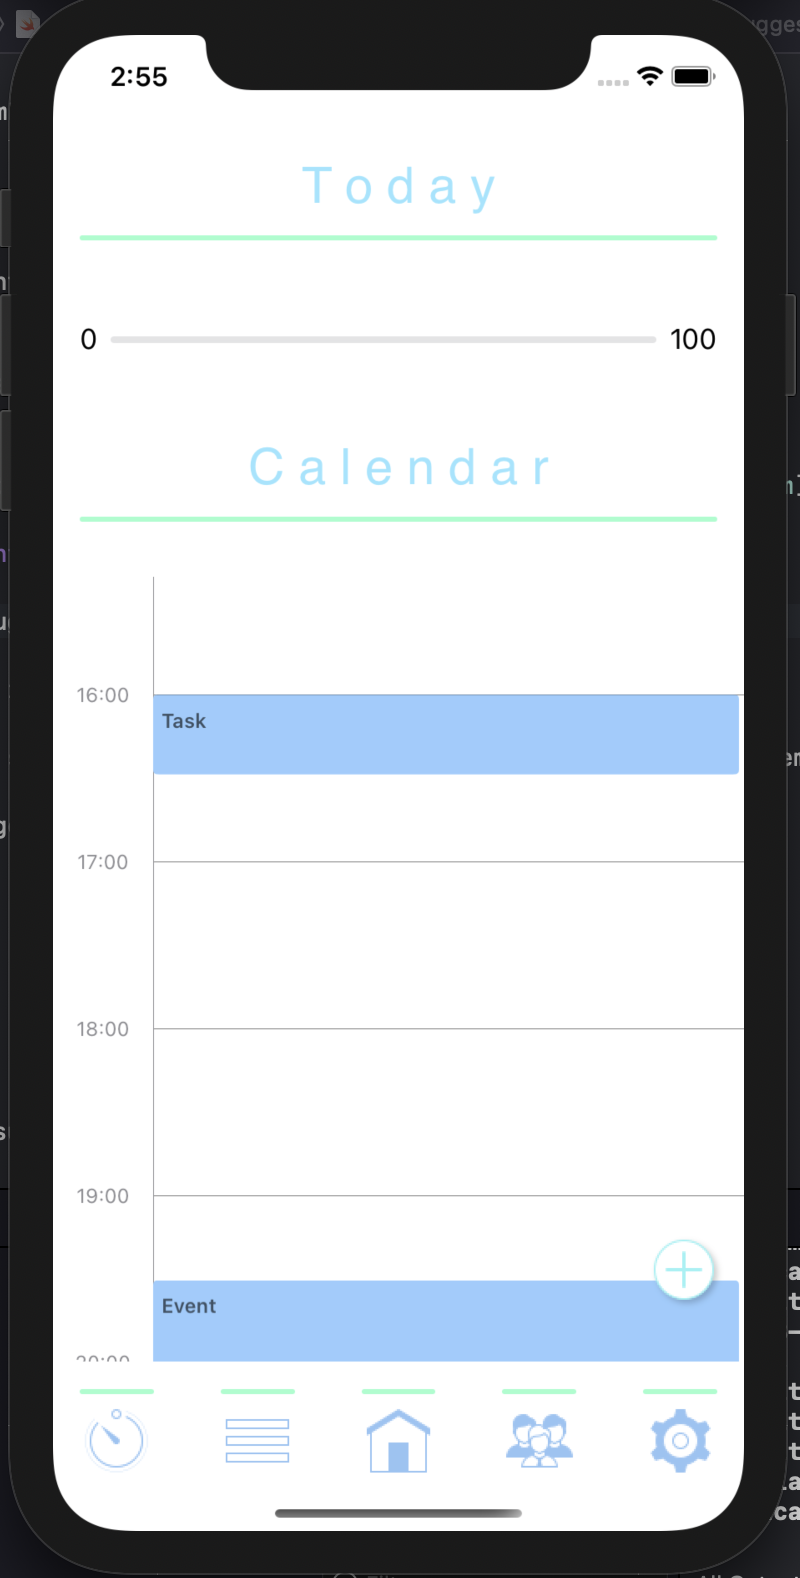
\includegraphics[width=\textwidth]{./graphics/Implementation/Dashboard/calendar today populated.png}
        \caption{Sign In.}
        \label{fig:calendar_today_app}
    \end{subfigure}
    
    \caption{The agenda and calendar today views.}
    \label{fig:agenda_calendar_today_app}
\end{figure}
        
        The agenda view for the other time frames is identical to the 'today' view. However, the calendar view for each time frame is slightly different.  The calendar for the 'today' time frame will show an hour-by-hour calendar for one day only.  This weeks' calendar will show an hour-by-hour calendar, but the user can choose from any day available during the week.  Finally, the calendar for this month shows a block for each day of the month, with a small dot indicator to show if there is an item during that day.  When the user taps on the day, a list of the items due will be shown below the calendar.
        
        When a user taps on a task in any of the calendar views, a view will appear on the screen with all the available details attached to that item and an option to edit the item.  If the user taps the edit button, they will be taken to the add item view. However, each element will already be populated with the item details, which can then be changed and saved.
        
        \begin{figure}[H]
    \centering
    \begin{subfigure}[b]{0.3\textwidth}
        \centering
        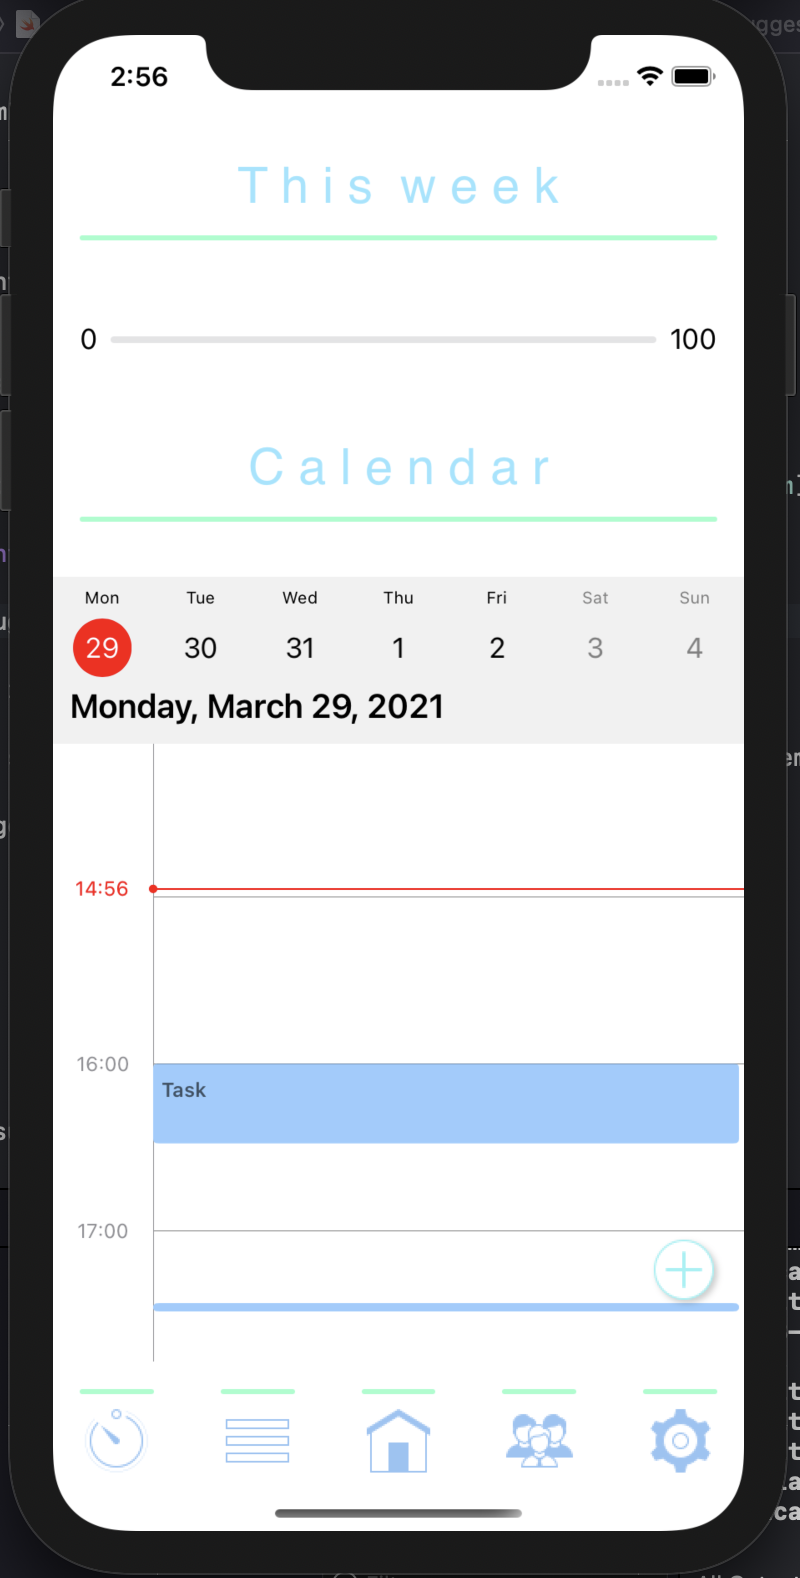
\includegraphics[width=\textwidth]{./graphics/Implementation/Dashboard/calendar this week populated.png}
        \caption{Calendar This Week.}
        \label{fig:cal_this_week_app}
    \end{subfigure}
    \hfill
    \begin{subfigure}[b]{0.3\textwidth}
        \centering
        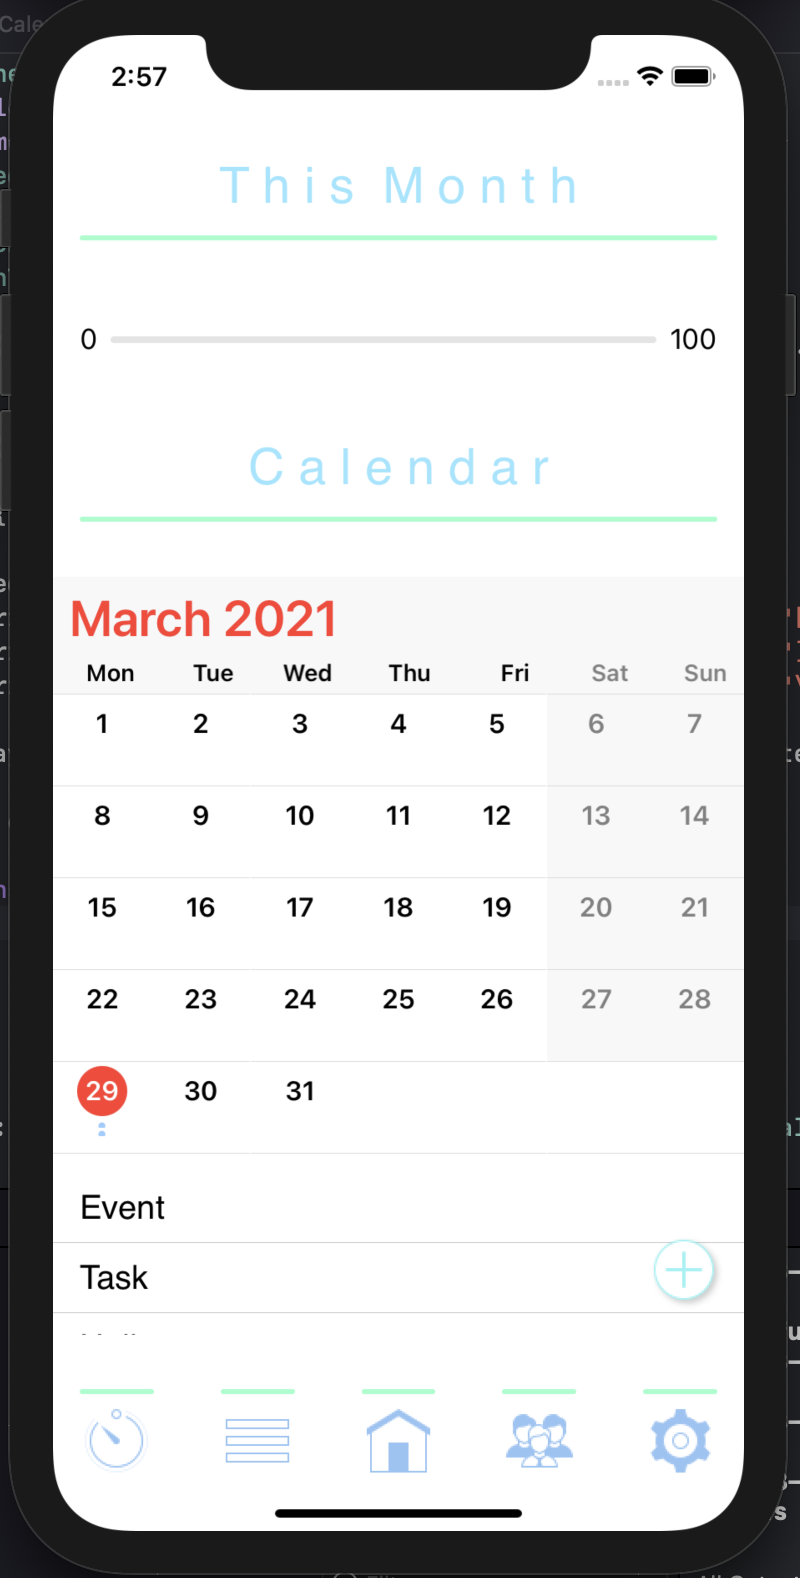
\includegraphics[width=\textwidth]{./graphics/Implementation/Dashboard/calendar this month populated.png}
        \caption{Calendar This Month.}
        \label{fig:cal_this_month_app}
    \end{subfigure}
    \hfill
    \begin{subfigure}[b]{0.3\textwidth}
        \centering
        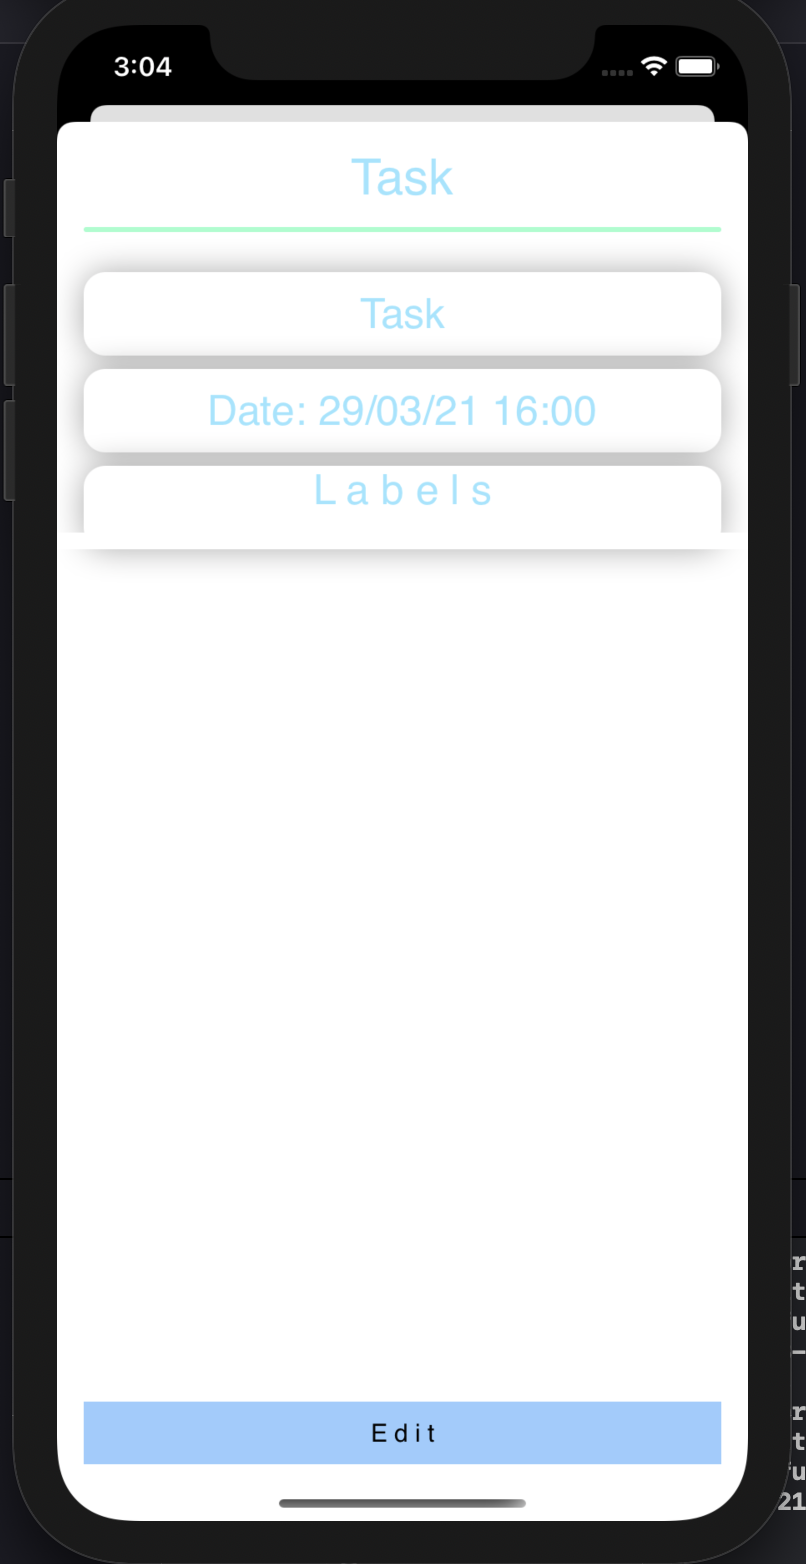
\includegraphics[width=\textwidth]{./graphics/Implementation/Dashboard/task detail.png}
        \caption{Item Detail View.}
        \label{fig:item_detail_app}
    \end{subfigure}
    
    \caption{The calendar views and item detail view.}
    \label{fig:cal_item_app}
\end{figure}
        
        \subsubsection{Back-end}
        \label{subsubsec:dashboard_backend}
        The FirebaseSession class primarily handles the adding and deleting of items and works with Item objects defined within the application to populate the views.  When the dashboard is brought to the foreground, the items stored under the user in the database need to be downloaded to the application. This is done using the retrieveItems function defined in the Firebase Session class.  This function calls the getDocument function in the API and using the document file path, all available items in that path of the database are downloaded.  Each element within the item is converted into the correct object, such as String, Bool, NSDate and added to an array of Item objects, then assigned to the User object to be accessed from within the application.  The function retrieveLabels does a similar task, just in the context of labels instead of items.  Finally, retrieveProgress repeats the task within the context of progress.
        
        When completing an item, the progress counter is incremented by one, and this is then saved to the database using the saveProgress function.  The setData function provided by the Firebase API is called, and this updates the progress value in the database to the correct value.  The boolean tracking whether the item is complete within the Item object is also set to true.  When something is changed in an Item object, the saveItem function is called in Firebase Session. Similarly to updating the progress, it will call the setData API function and update the database with the correct information.  Finally, if the user wishes to delete an item entirely, they can swipe either left or right on that item, which will trigger the deleteItem function.  This calls the document function from the API to locate the relevant item in the database. If this is successfully found, the API's delete function is called, which deletes the item from the database.  The source code snippets for the functions mentioned can be found in the appendix under Section~\ref{app:dashboard_backend}.
        
        \subsection{Add Item}
        \subsubsection{Front-end}
        The add item view is mainly made up of toggle objects within a ScrollView.  The user can type in the name of their desired item in the title text field, which is a custom TextField with a HorizontalLine object as the coloured underline.  The user can then toggle their desired options; if the date or reminder toggle is switched on, a DatePicker object appears in order for a date and time to be chosen, and if the even toggle is switched on, a time interval picker appears to choose the length of time the item will last.  At the bottom of the view, the user can add labels to the item.  When they tap the '+' button, a text field will appear to type the new labels' name, and once they tap the tick button, they can then tap the newly created label, which will be highlighted to show it has been selected.  Once the add button is tapped, the application will return to the dashboard, and the newly added item will be able to be viewed.
        
        Suppose the user decides to set a reminder. In that case, once the add button has been tapped, they will be asked permission by iOS to send them notifications from the application (if this has not already been allowed or disallowed).  Once allow has been tapped, reminders will appear in the devices notification centre at the relevant times.  An example of this can be seen in Figure~\ref{fig:add_item_notifications}.
        
        \begin{figure}[H]
    \centering
    \begin{subfigure}[b]{0.3\textwidth}
        \centering
        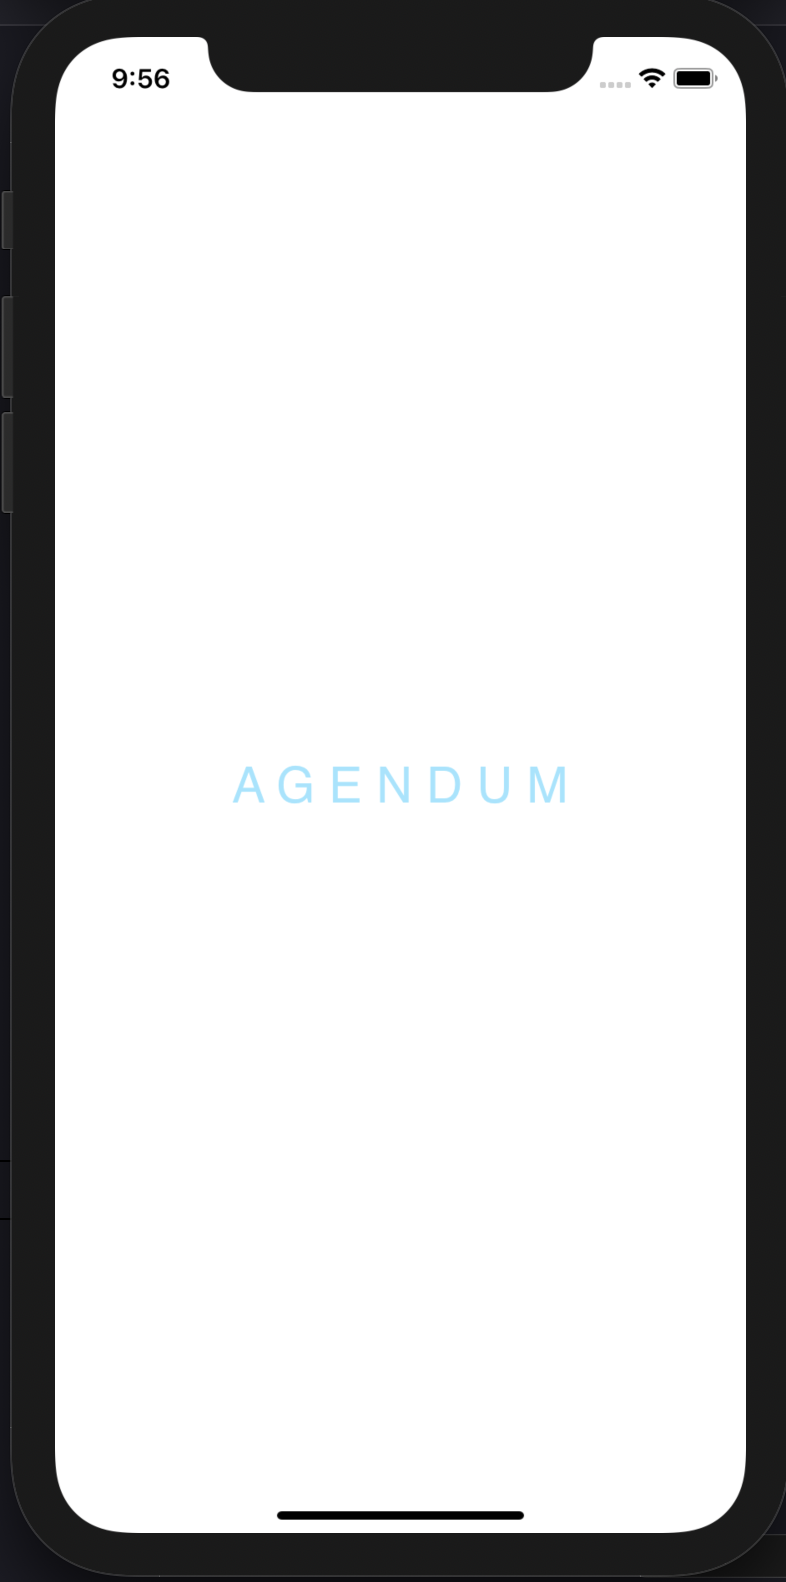
\includegraphics[width=\textwidth]{./graphics/Implementation/Splash_Sign_Up_Sign_In/splash.png}
        \caption{Splash Screen.}
        \label{fig:splash_app}
    \end{subfigure}
    \hfill
    \begin{subfigure}[b]{0.3\textwidth}
        \centering
        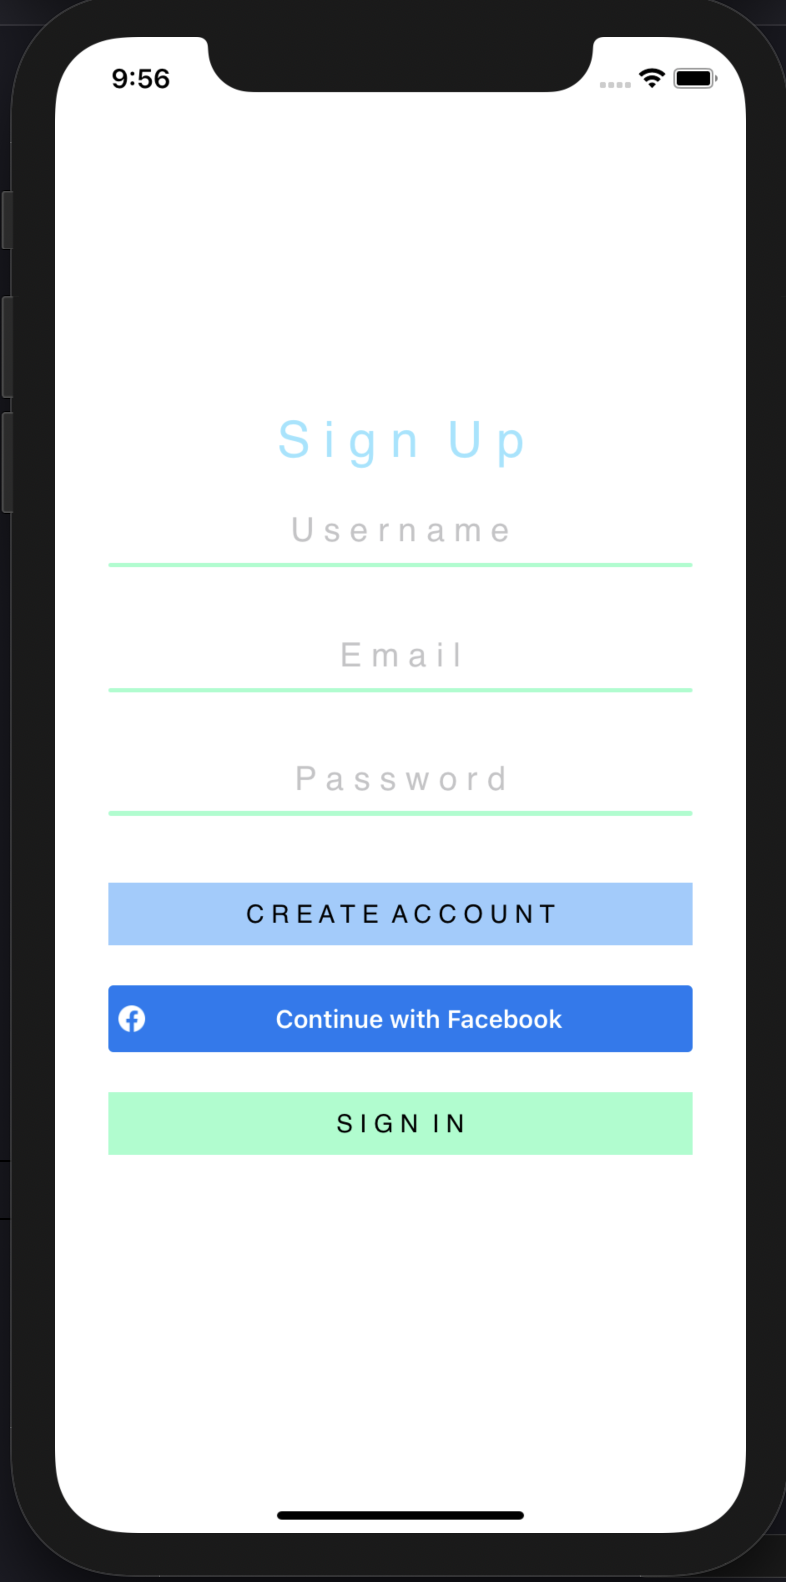
\includegraphics[width=\textwidth]{./graphics/Implementation/Splash_Sign_Up_Sign_In/signup.png}
        \caption{Sign Up.}
        \label{fig:sign_up_app}
    \end{subfigure}
    \hfill
    \begin{subfigure}[b]{0.3\textwidth}
        \centering
        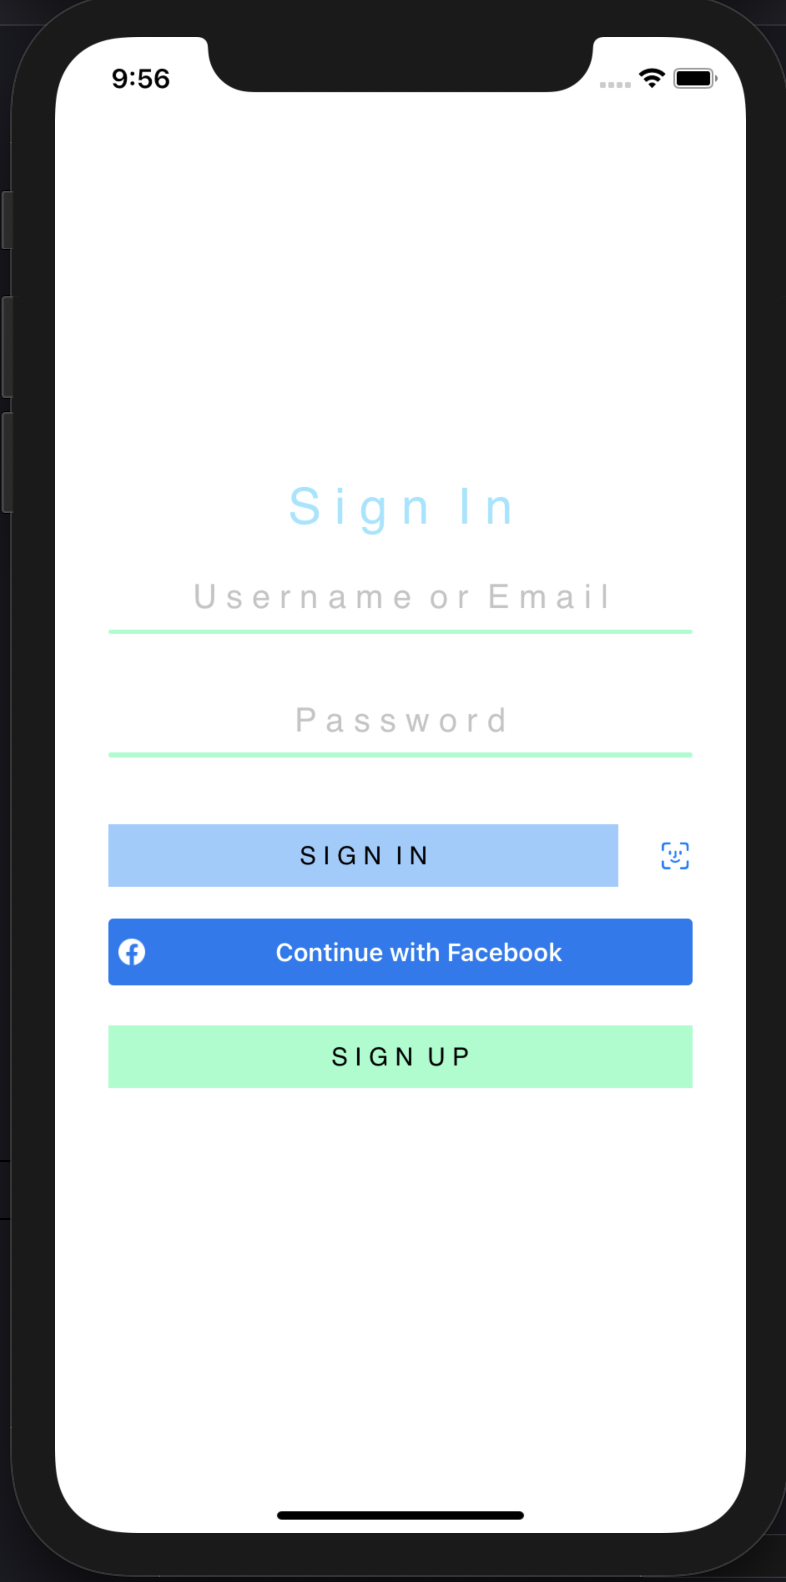
\includegraphics[width=\textwidth]{./graphics/Implementation/Splash_Sign_Up_Sign_In/signin.png}
        \caption{Sign In.}
        \label{fig:sign_in_app}
    \end{subfigure}
    
    \caption{Splash, sign up and sign in views shown in the application.}
    \label{fig:splash_signup_signin_app}
\end{figure}
        
        \subsubsection{Back-end}
        The addItem function defined in the FirebaseSession class handles saving the new item to the database, which is explained in more detail in Section~\ref{subsubsec:dashboard_backend}.
        
        The Notifications class handles the creation of notifications, and an instance of this class is called when the add button is tapped.  The requestPermissions function is called, which generates the alert to allow or deny permissions for notifications to be sent from the application.  If permissions have already been granted, the alert box is not shown.  The generateNotification function then creates the relevant notification by setting a title, and description for the notification and the action, which is performed when the notification is tapped.  It is then added to a notification queue and is released at the desired time.  Apart from what is defined in the application, the notification system is entirely handled by iOS.  The Notifications class code snippets can be seen in Section~\ref{app:add_item_backend} of the appendix.
        
        \subsection{Focus}
        \subsubsection{Front-end}
        The focus view uses the SwiftUIPager framework in order for the user to be able to swipe from the main timer view to the settings.  Within the main view, a custom timer uses the Timer class provided in the Combine framework to countdown from a specified time.  The begin button triggers the countdown and changes to a pause button in order to allow the user to pause the timer.  The break button switches the timer to the desired amount of time the user has set for a break, and the reset button sets the timer back to the original time.  Below these buttons is a text object which shows the item (if one has been selected) that the user has chosen to focus on.
        
        When the user swipes to the left on the timer, they are taken to the settings to set the focus time and the break time.  When either of these items is tapped, a Picker object becomes visible where the user can choose the length of time they wish to set.  Below this, a list of tasks are shown that are yet to be completed; if a user taps on one of these, it will become highlighted, and swiping right on this view will take the user back to the newly set timer.  This functionality can be seen in Figure~\ref{fig:focus_app}.
        
        \begin{figure}[H]
    \centering
    \begin{subfigure}[b]{0.3\textwidth}
        \centering
        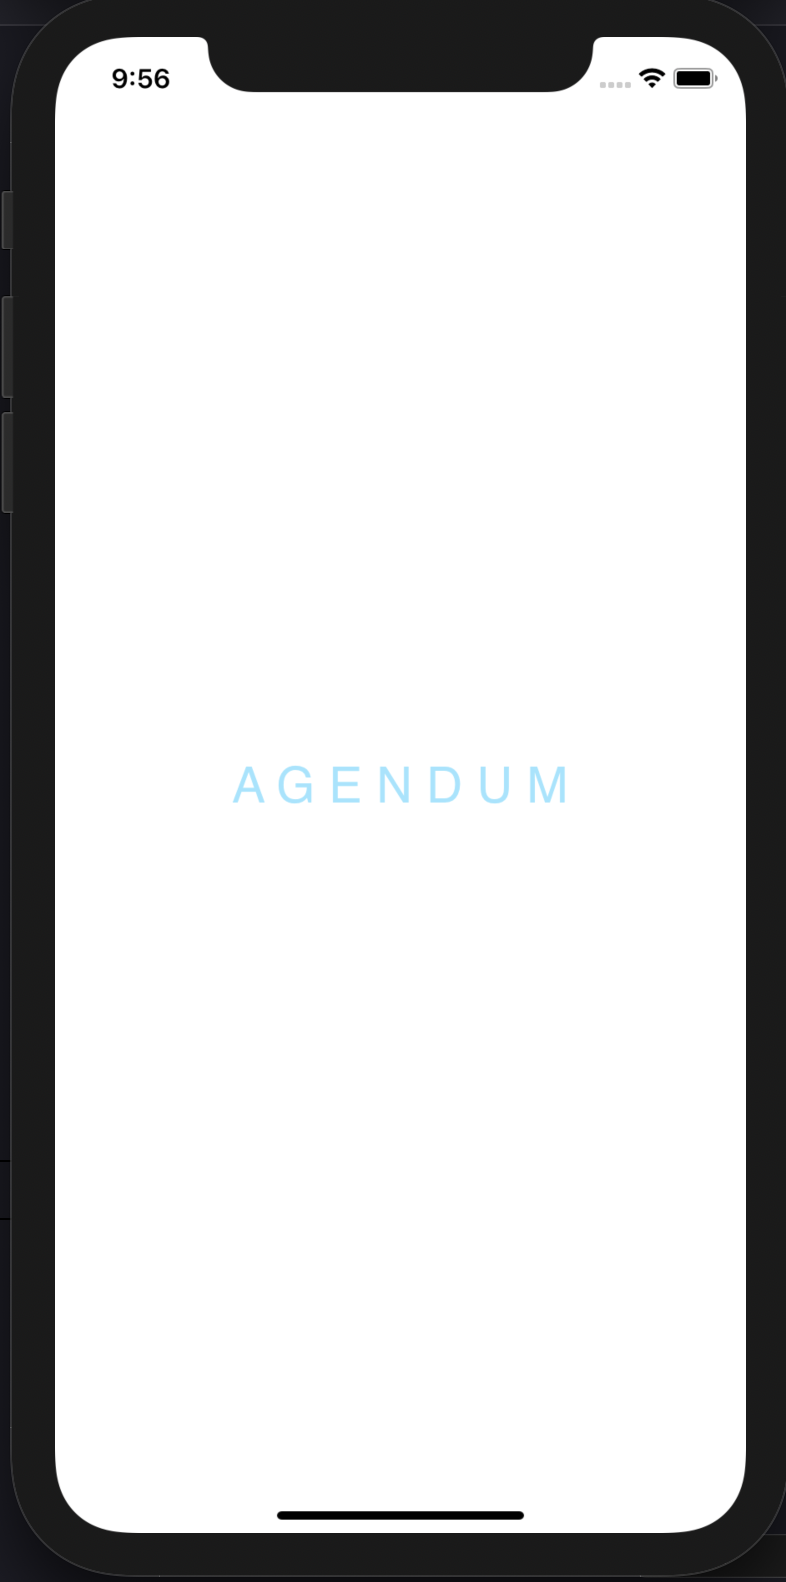
\includegraphics[width=\textwidth]{./graphics/Implementation/Splash_Sign_Up_Sign_In/splash.png}
        \caption{Splash Screen.}
        \label{fig:splash_app}
    \end{subfigure}
    \hfill
    \begin{subfigure}[b]{0.3\textwidth}
        \centering
        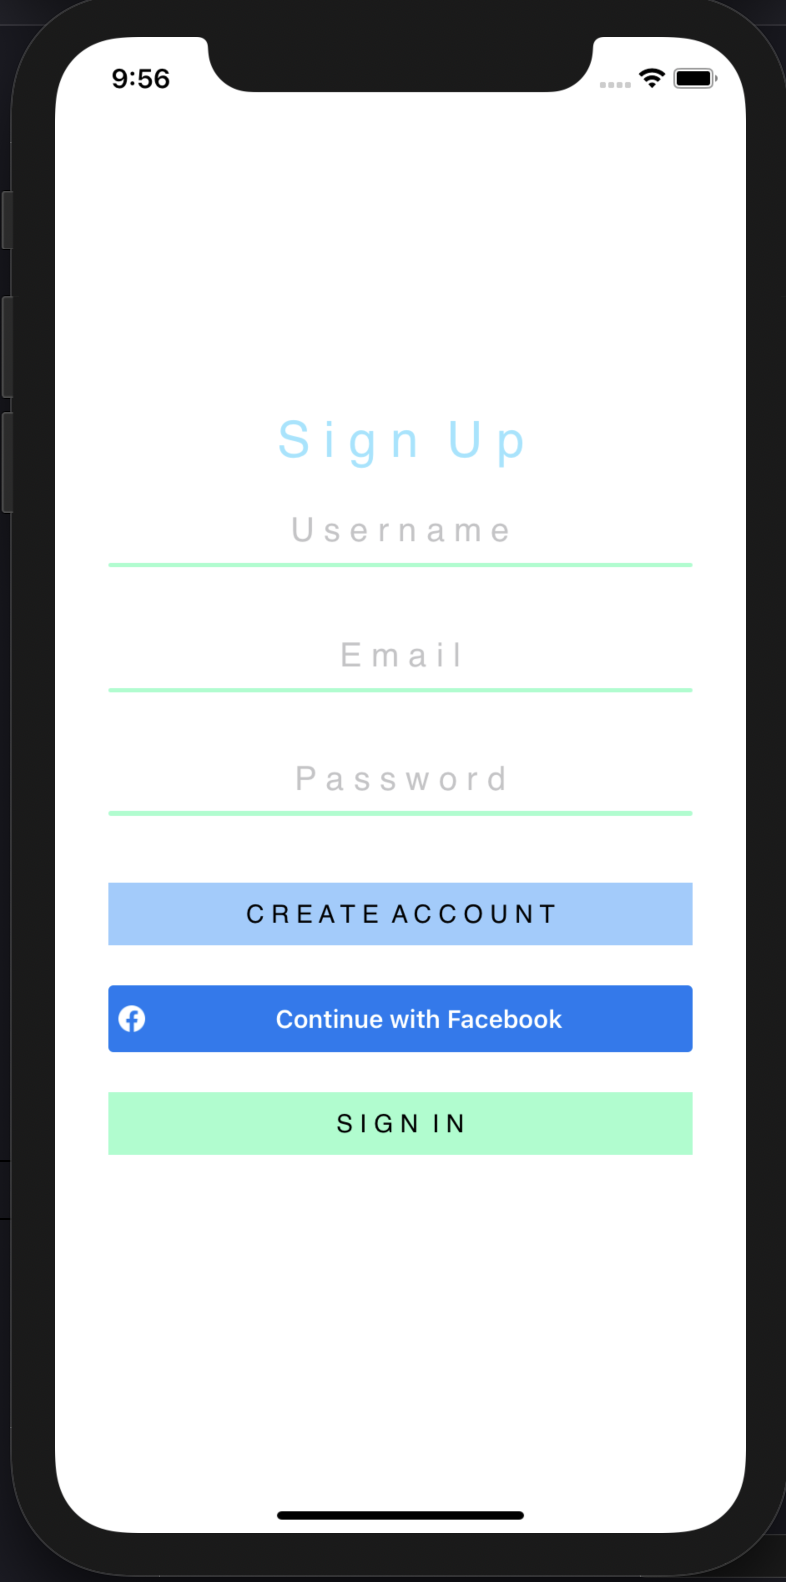
\includegraphics[width=\textwidth]{./graphics/Implementation/Splash_Sign_Up_Sign_In/signup.png}
        \caption{Sign Up.}
        \label{fig:sign_up_app}
    \end{subfigure}
    \hfill
    \begin{subfigure}[b]{0.3\textwidth}
        \centering
        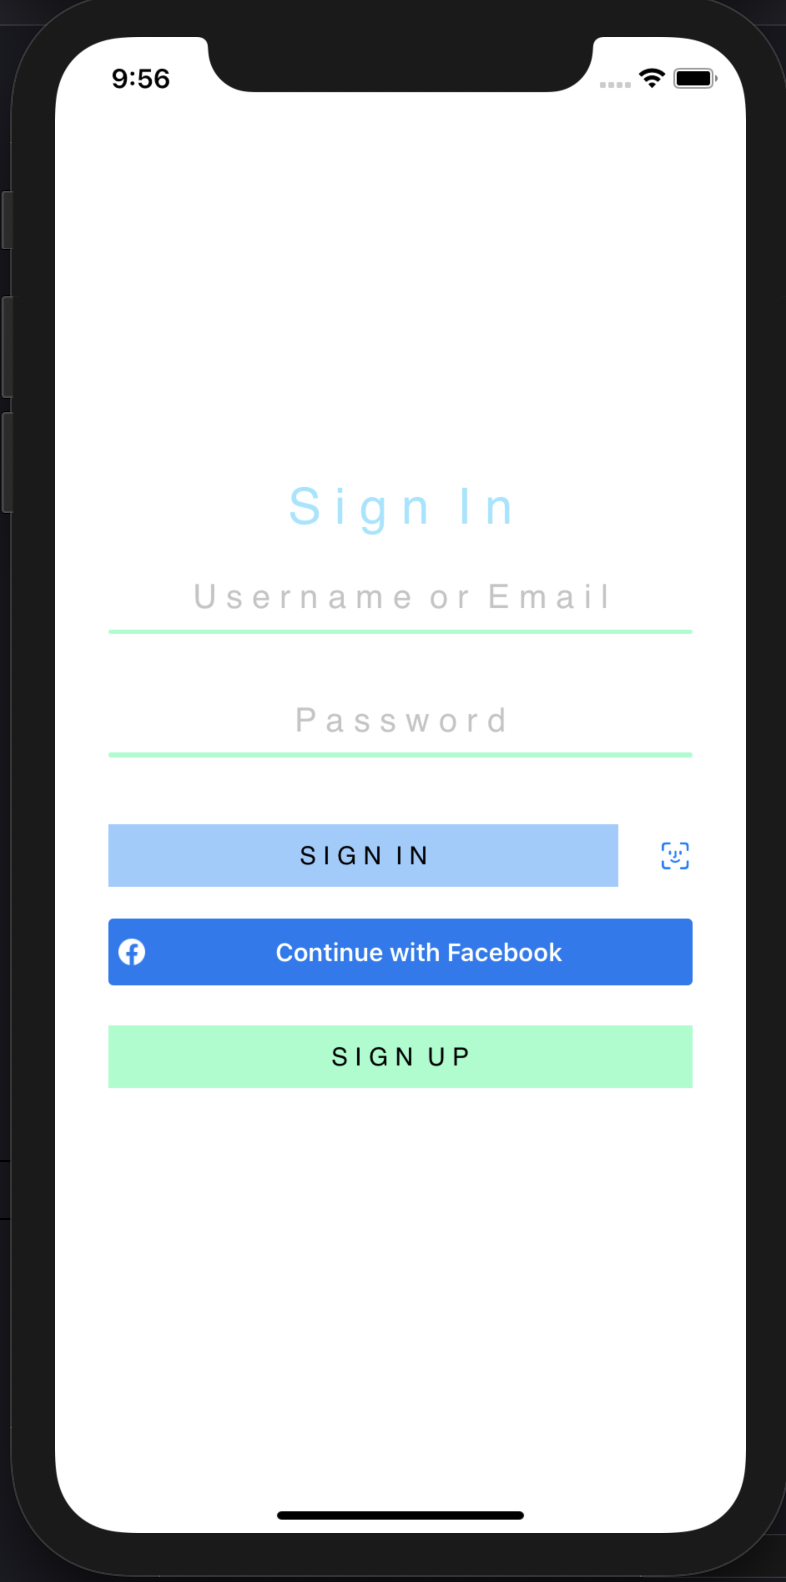
\includegraphics[width=\textwidth]{./graphics/Implementation/Splash_Sign_Up_Sign_In/signin.png}
        \caption{Sign In.}
        \label{fig:sign_in_app}
    \end{subfigure}
    
    \caption{Splash, sign up and sign in views shown in the application.}
    \label{fig:splash_signup_signin_app}
\end{figure}
        
        \subsubsection{Back-end}
        The focus timers' functionality is handled chiefly within the view itself since defining a timer in SwiftUI does not require much computation.  However, to retrieve the tasks in the focus settings, the retrieveItems function is called from the FirebaseSession class.  Details of this function have already been discussed in Section~\ref{subsubsec:dashboard_backend}.
        
        \subsection{All Items}
        \subsubsection{Front-end}
        The All Items view is relatively simple as it is effectively just a list of all the items the user has created.  If an item is not a habit, labelled or has no date set, it will appear in random order at the top of the view.  Items that are due within the next seven days are placed under the 'Due Soon' heading, habits are placed under the 'Habit' heading, items that have been labelled are placed under the title with the name of the label, and items that have been completed are placed under the 'completed' heading.  Tapping the filter button on the left of the search bar will place the items in alphabetical order.  The user can also search for specific items by typing into the search bar.  In Figure~\ref{fig:all_items_app}, an example of this is shown in image C; the user has typed the letter 'E', and items beginning with that letter have been filtered, in this case, an item named 'Event'.
        
        \begin{figure}[H]
    \centering
    \begin{subfigure}[b]{0.3\textwidth}
        \centering
        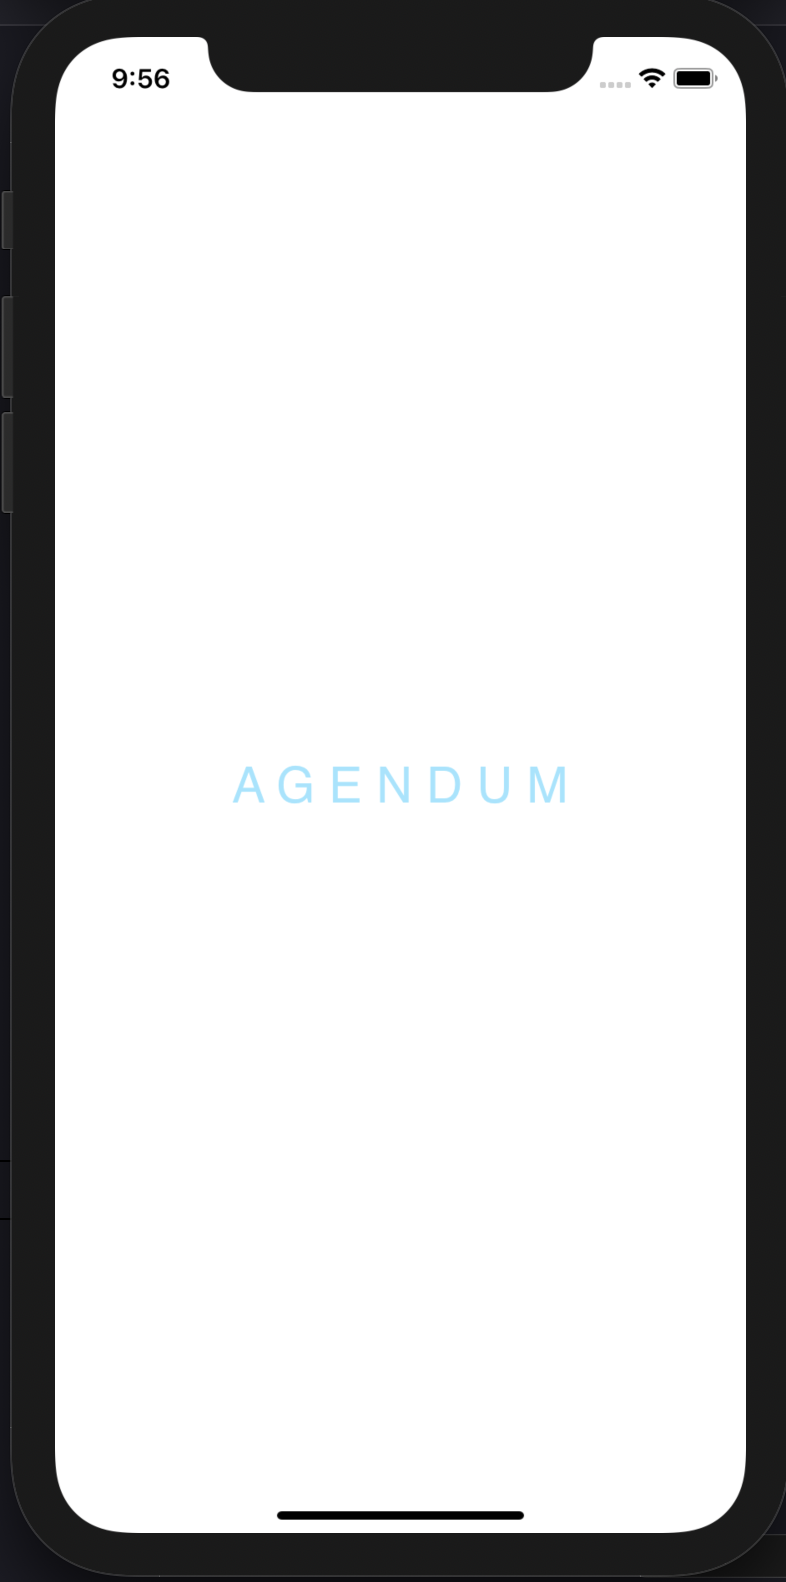
\includegraphics[width=\textwidth]{./graphics/Implementation/Splash_Sign_Up_Sign_In/splash.png}
        \caption{Splash Screen.}
        \label{fig:splash_app}
    \end{subfigure}
    \hfill
    \begin{subfigure}[b]{0.3\textwidth}
        \centering
        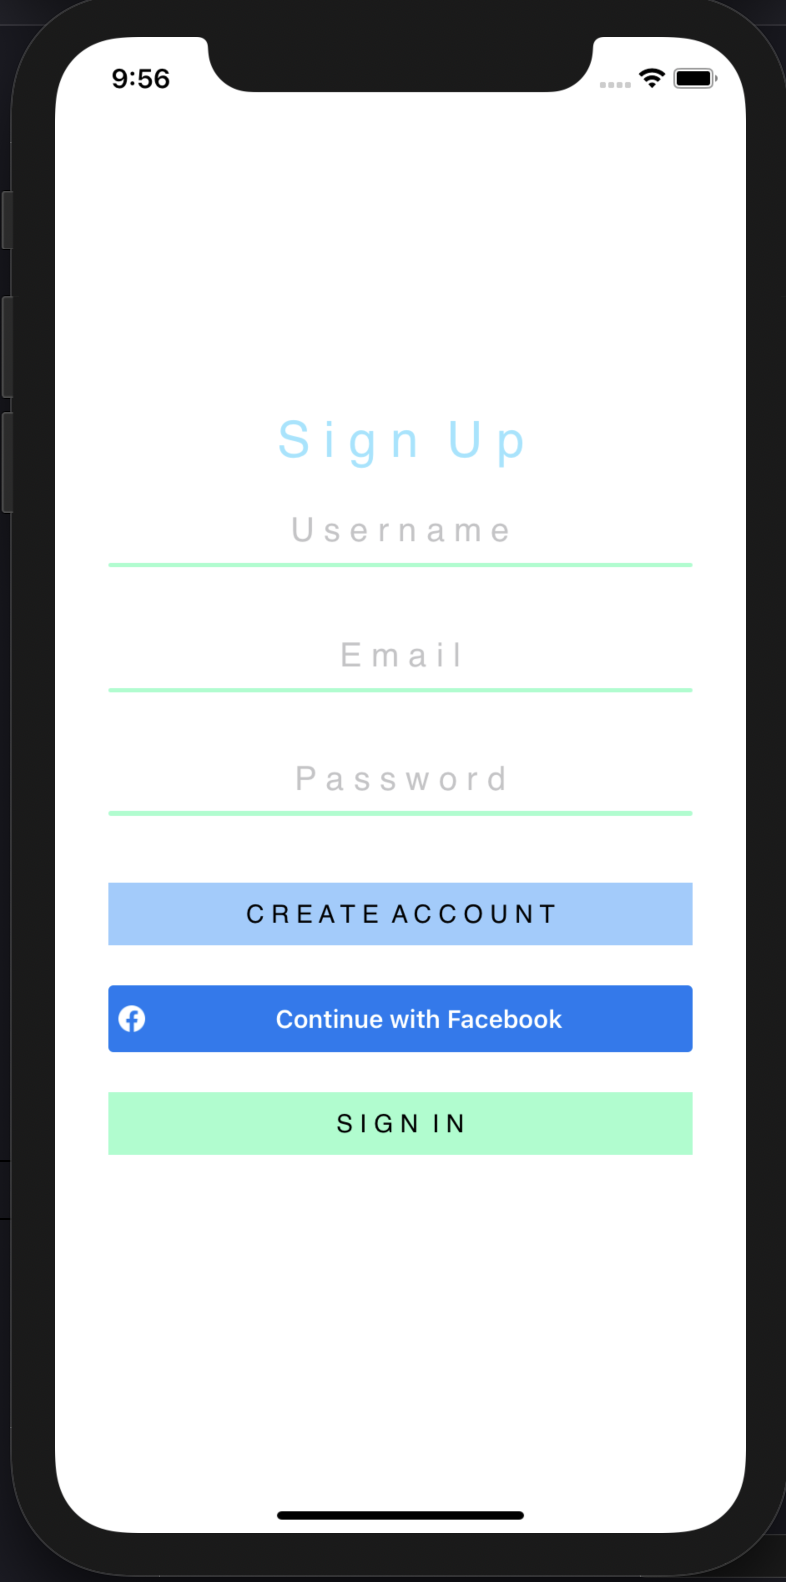
\includegraphics[width=\textwidth]{./graphics/Implementation/Splash_Sign_Up_Sign_In/signup.png}
        \caption{Sign Up.}
        \label{fig:sign_up_app}
    \end{subfigure}
    \hfill
    \begin{subfigure}[b]{0.3\textwidth}
        \centering
        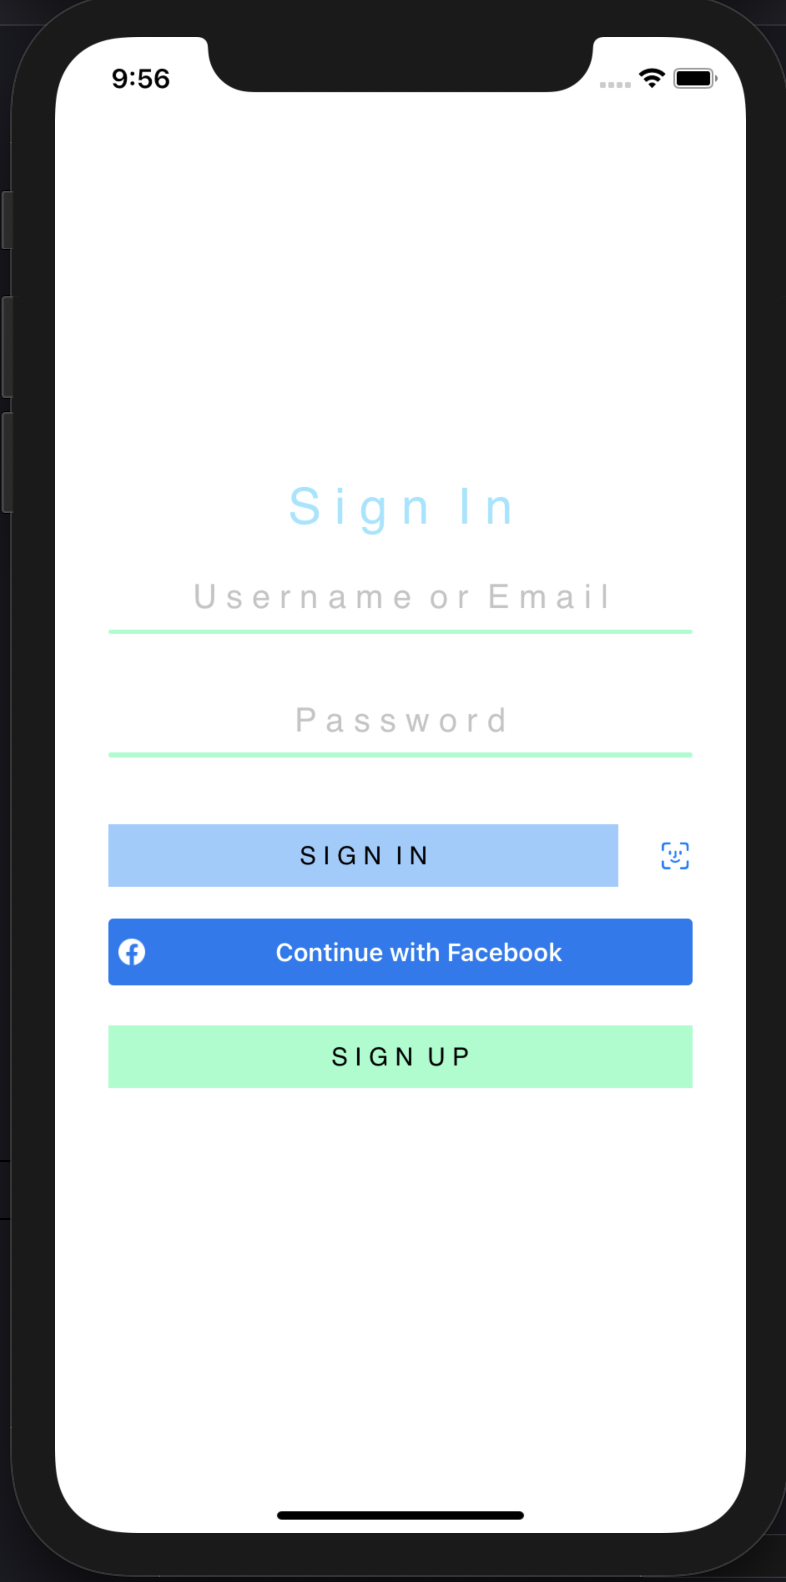
\includegraphics[width=\textwidth]{./graphics/Implementation/Splash_Sign_Up_Sign_In/signin.png}
        \caption{Sign In.}
        \label{fig:sign_in_app}
    \end{subfigure}
    
    \caption{Splash, sign up and sign in views shown in the application.}
    \label{fig:splash_signup_signin_app}
\end{figure}
        
        The view also contains an add button, which will take the user to the add item view.
        
        \subsubsection{Back-end}
        The retrieveItems function defined in the FirebaseSession class is used to download a list of Item objects, which are then parsed to display the items in the view.  The filtering and searching of items are handled in the view source files since they do not require much computation.  Both of them loop through the list of items and extract the relevant items depending on the search/filtering criteria.
        
        \subsection{Friends}
        \subsubsection{Front-end}
        The 'friends' view contains a list of users that the current user has added.  The users' email alongside their current progress points are shown, and at the bottom of the view is the logged in users' progress points.  When the user taps the add button they are taken to the add friend view, where there is a text field to input the user email they wish to add.  Once the user taps the submit button, they are taken back to the main 'friends' view; if the user they added was found it will be shown in their list of friends.  The user can also tap on a friend to be taken to the 'friends detail' view, which shows the friends' progress points and a delete button at the bottom of the view.  If the user taps the delete button, the friend will be removed from their friends list.
        
        \begin{figure}[H]
    \centering
    \begin{subfigure}[b]{0.3\textwidth}
        \centering
        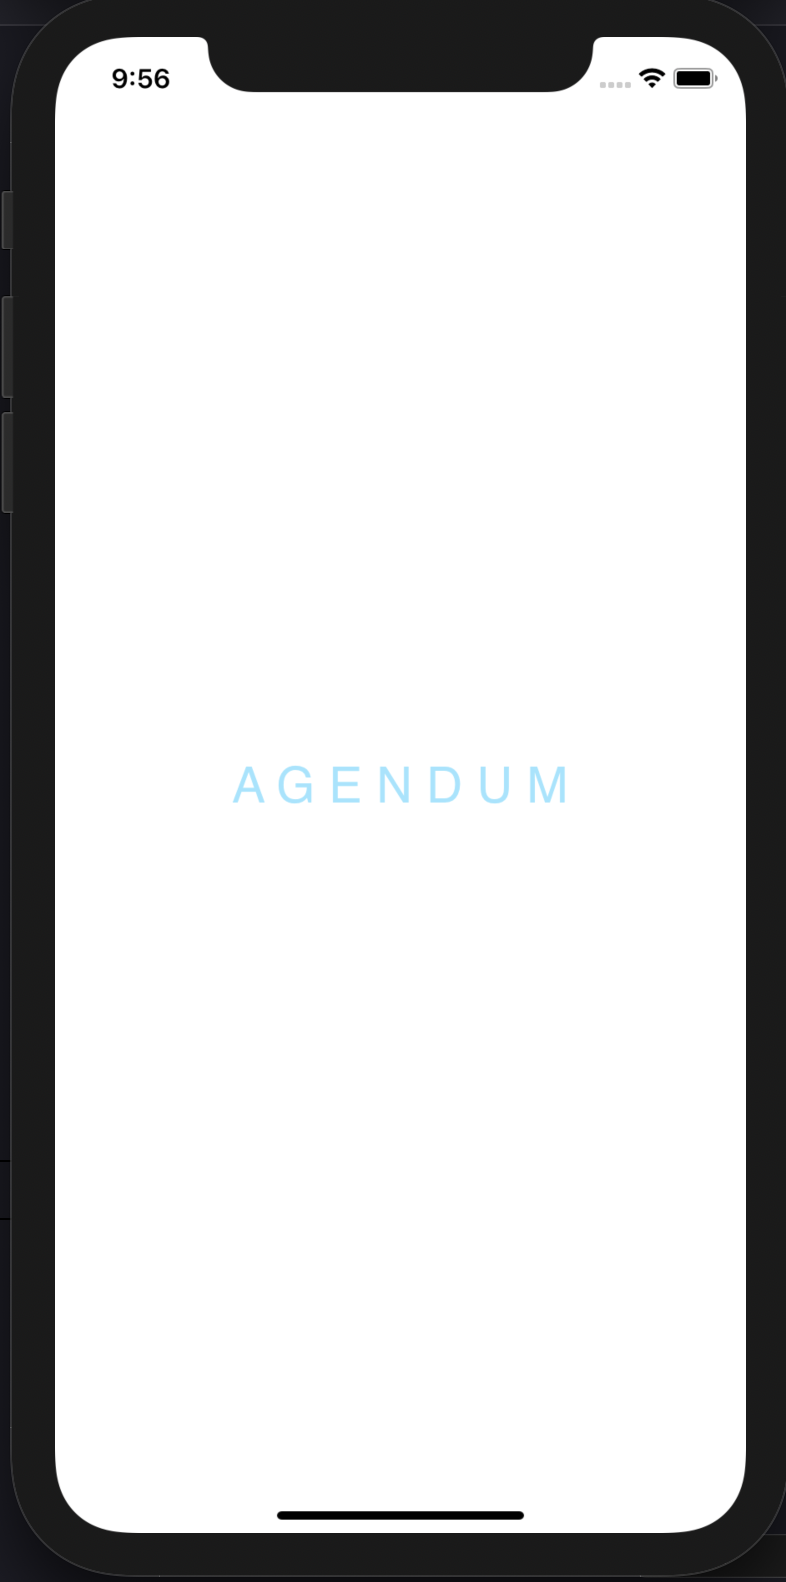
\includegraphics[width=\textwidth]{./graphics/Implementation/Splash_Sign_Up_Sign_In/splash.png}
        \caption{Splash Screen.}
        \label{fig:splash_app}
    \end{subfigure}
    \hfill
    \begin{subfigure}[b]{0.3\textwidth}
        \centering
        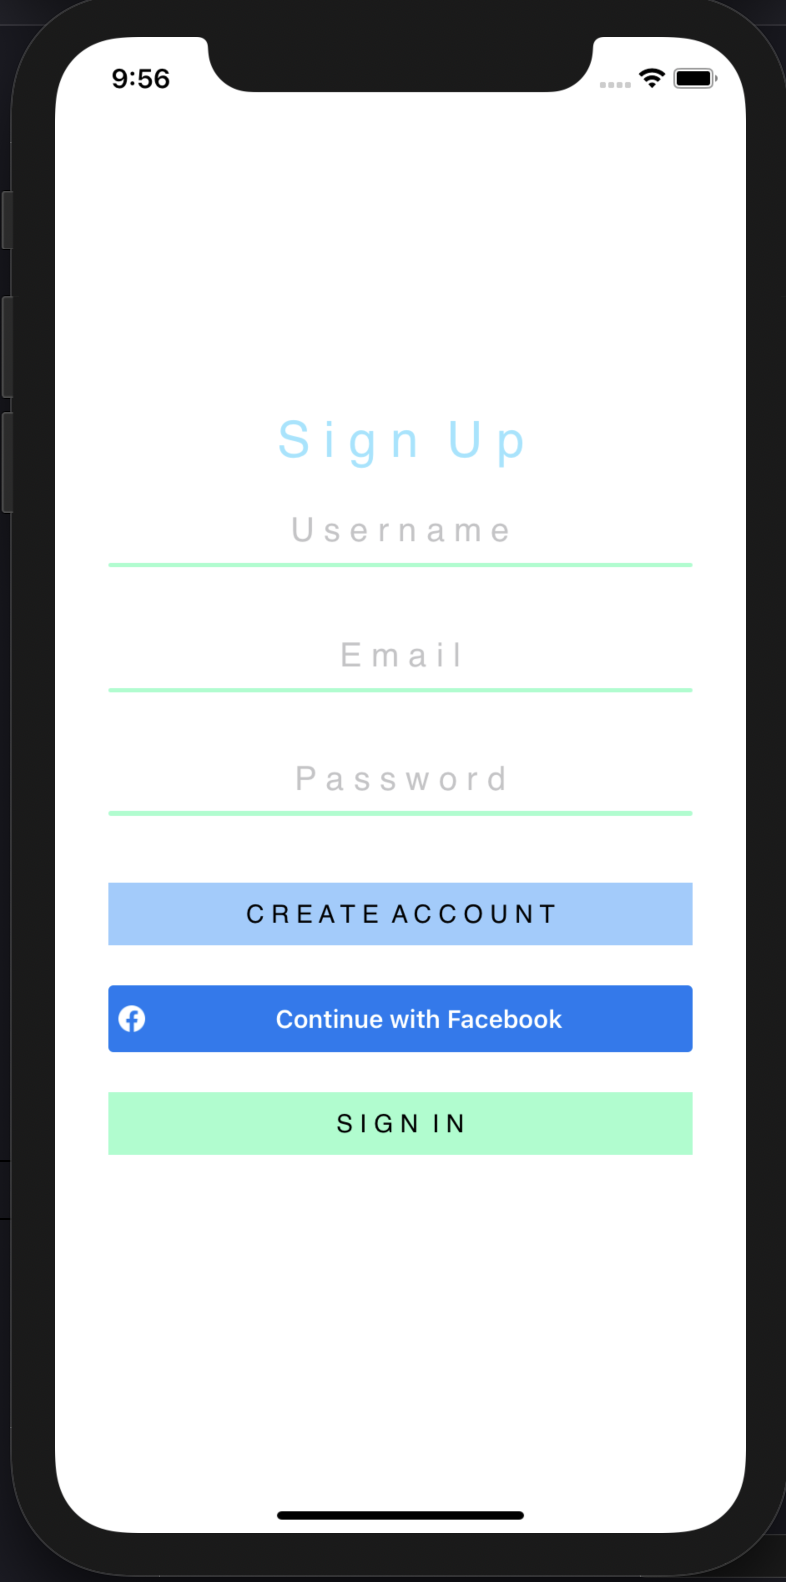
\includegraphics[width=\textwidth]{./graphics/Implementation/Splash_Sign_Up_Sign_In/signup.png}
        \caption{Sign Up.}
        \label{fig:sign_up_app}
    \end{subfigure}
    \hfill
    \begin{subfigure}[b]{0.3\textwidth}
        \centering
        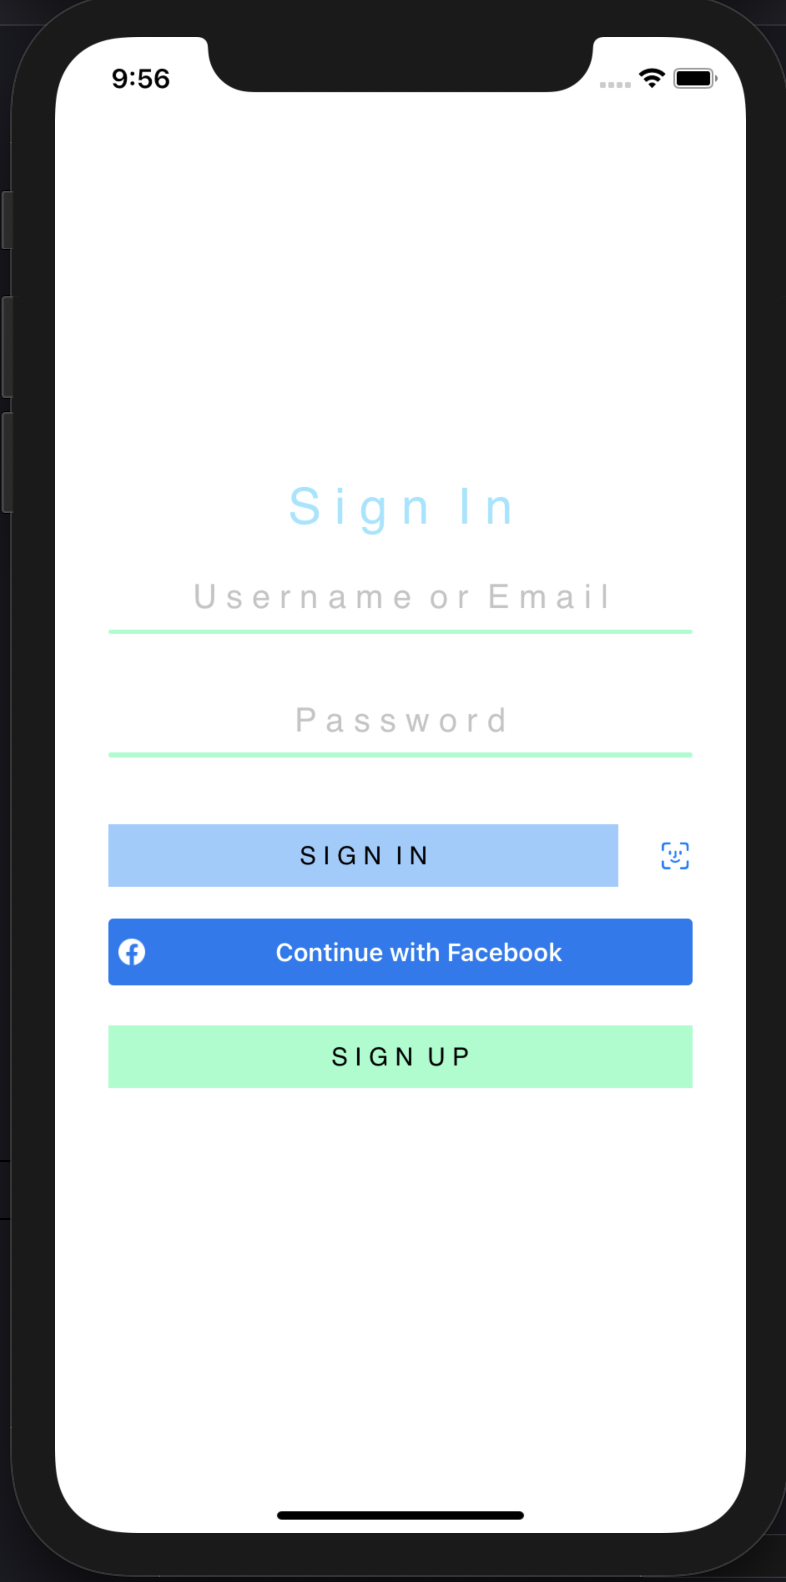
\includegraphics[width=\textwidth]{./graphics/Implementation/Splash_Sign_Up_Sign_In/signin.png}
        \caption{Sign In.}
        \label{fig:sign_in_app}
    \end{subfigure}
    
    \caption{Splash, sign up and sign in views shown in the application.}
    \label{fig:splash_signup_signin_app}
\end{figure}
        
        \subsubsection{Back-end}
        In order to add friends, the findUser function was added to the FirebaseSession class. The findUser function would use the getDocument API call to get a list of available users in the database.  The getDocuments API call would then be made to get the progress and user ID value stored under the user email to be found.  Once this is successful, the followUser function that is also stored in the FirebaseSession class is called.  The followUser function uses the setData API call to add the found user to the logged in users' database so that this information can be downloaded and displayed in the 'friends' view.
        
        If the user wishes to delete a friend, the unfollowUser function is called from the FirebaseSession class.  This function is almost identical to the findUser function, except once the getDocuments call is successful, the data is deleted from the current users' database rather than added.  The code snippets for these functions can be found in Section~\ref{app:friends_backend} of the appendix.
        
        \subsection{Settings}
        \subsubsection{Front-end}
        The settings view is contained of primarily buttons.  From the settings, the user can change their email and password and connect the iOS calendar, log out, delete their account, and activate bio-metric authentication.  When a user taps on either the change email or change password button, they will be asked to re-authenticate as this is a requirement of changing sensitive data in the Firebase database.  Therefore a pop-up will appear to allow the user to enter their password (or the bio-metric pop-up will appear if bio-metrics is enabled).  Once the user is authenticated, a pop-up will appear to change the email or password depending on which button was tapped.
        
        \begin{figure}[H]
    \centering
    \begin{subfigure}[b]{0.3\textwidth}
        \centering
        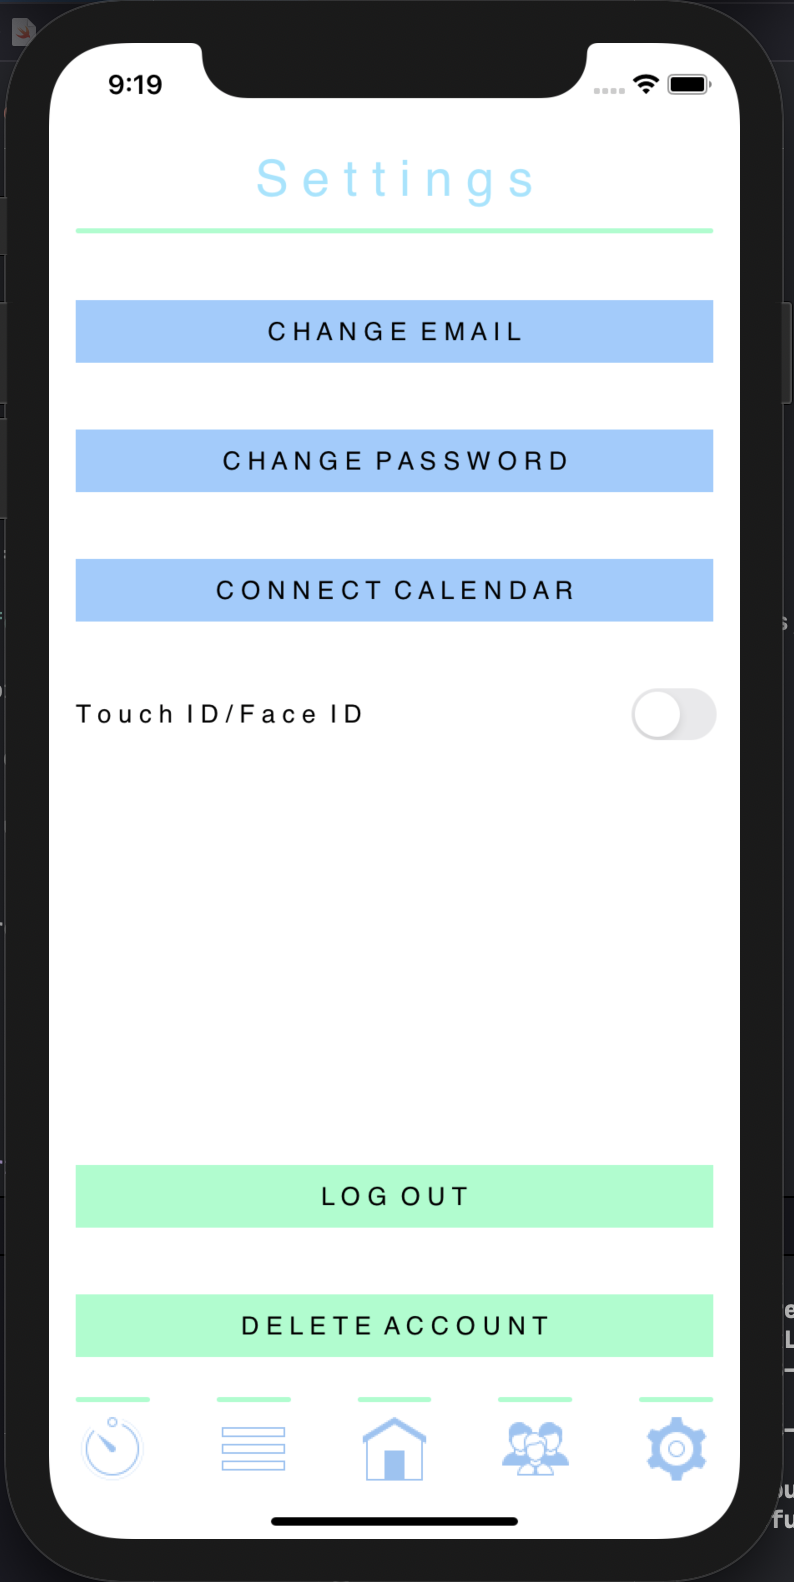
\includegraphics[width=\textwidth]{./graphics/Implementation/Settings/settings.png}
        \caption{Settings View.}
        \label{fig:settings_app}
    \end{subfigure}
    \hfill
    \begin{subfigure}[b]{0.3\textwidth}
        \centering
        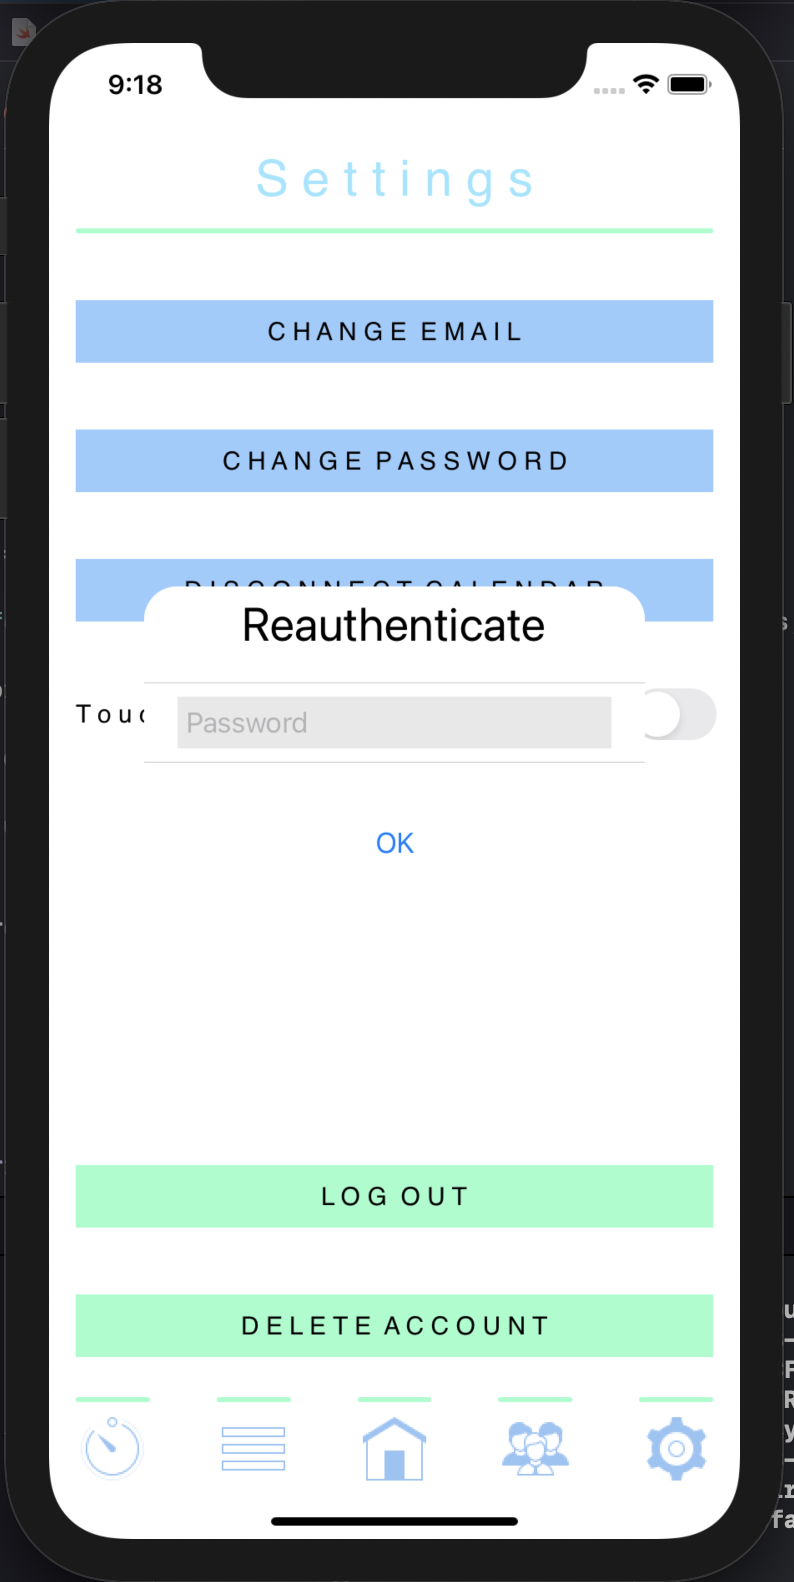
\includegraphics[width=\textwidth]{./graphics/Implementation/Settings/reauth.png}
        \caption{Re-authenticate pop-up.}
        \label{fig:reauth_app}
    \end{subfigure}
    \hfill
    \begin{subfigure}[b]{0.3\textwidth}
        \centering
        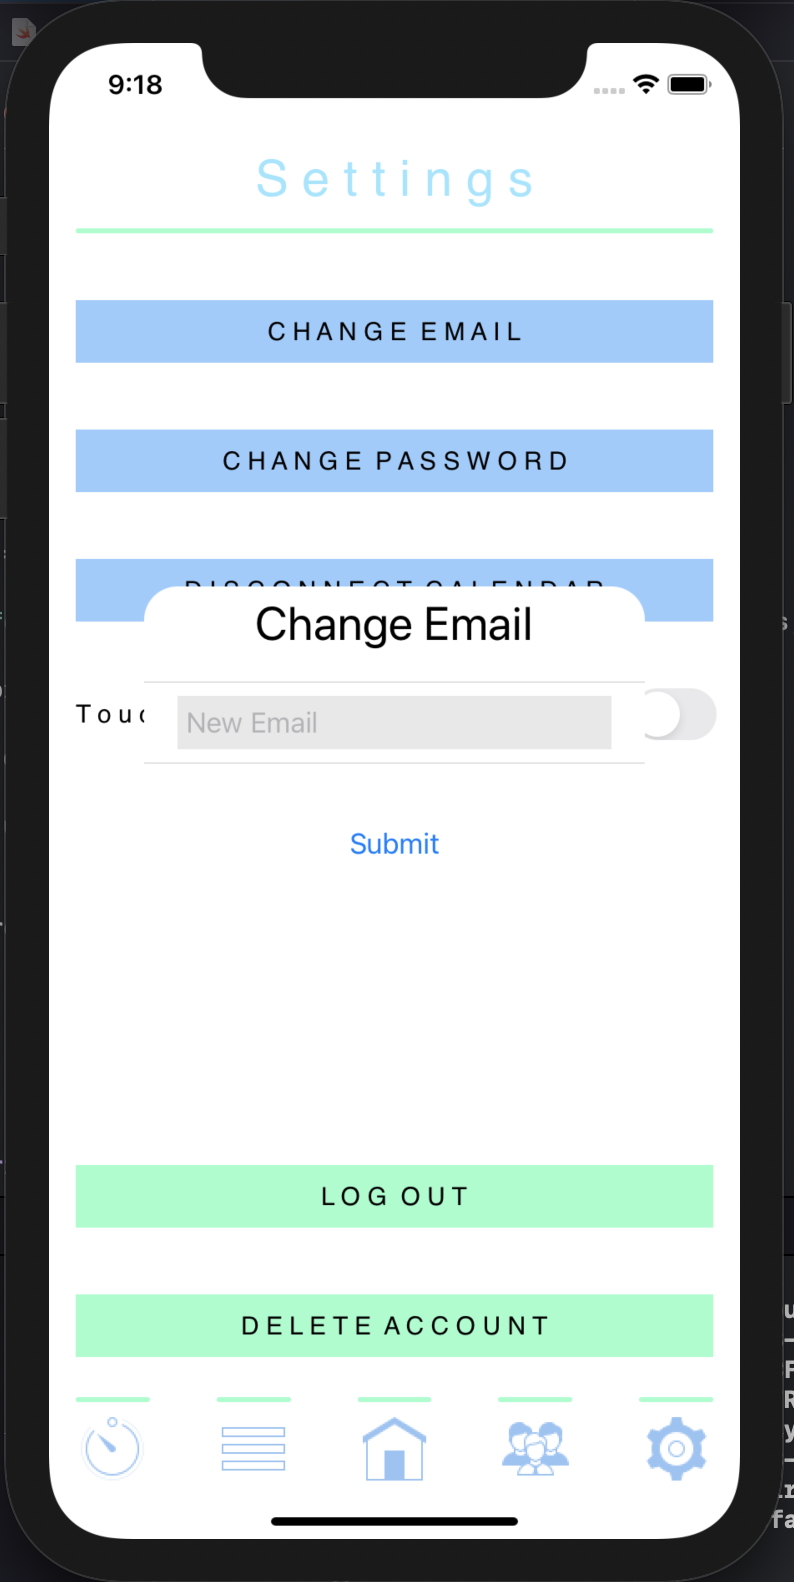
\includegraphics[width=\textwidth]{./graphics/Implementation/Settings/change email.png}
        \caption{Change Email pop-up.}
        \label{fig:change_email_app}
    \end{subfigure}
    
    \caption{Settings View, Re-authenticate and Change Email pop-ups.}
    \label{fig:settings_reauth_change_email}
\end{figure}
        
        Suppose the user toggles the Touch ID/Face ID toggle. In that case, they will be asked to authenticate using the method of biometric authentication on the device (the device used in the project had face ID authentication).  The password pop-up and bio-metric authentication can be found in Section~\ref{app:settings_frontend} of the appendix.  The user can tap the log out button to be taken to the sign-in view or tap the delete button, which will once again cause the application to ask for re-authentication, and once successful; it takes the user to the sign-in screen.
        
        \subsubsection{Back-end}
        To handle the biometric authentication, the Biometrics class was created.  The iOS system mainly handles the bio-metrics, but the tryBiometricAuthentication function will first check whether it is possible to try bio-metric authentication and, if so, generate the touch ID/face ID pop-up so that the user can authenticate.  If it fails, iOS will prompt the user to try again, and if successful, the application will return to the settings screen.  The faceIDAvailable function simply checks what iOS version is installed on the device; if it is newer than iOS11 and the required hardware is available, the function will return true.
        
        When the user wants to change their password, it will be changed both in the Firebase database and in the Apple Keychain storage.  When updating the password in Keychain, the updateGenericPasswordFor function will be called in the KeychainWrapper class, which will find where the password is stored and replace it with the new one.  This function is called from the updatePassword function in the FirebaseSession class after the updatePassword API call is successful.
        
        When the user wishes to change their email, the updateEmail function in FirebaseSession will be called. Similarly to updatePassword, the updateEmail API call will be made to the Firebase database.  In both scenarios, the re-authenticate function will be called, which requires an AuthCredential object as a parameter in order to ensure the user is authenticated to perform sensitive operations in the database.  This is done simply by retrieving the email already stored in the user object and then extracting the password that the user had re-input into the password prompt.
        
        When the user wishes to delete their account, the delete function will be called in the FirebaseSession class.  This calls another function named deleteUserData in FirebaseSession, which deletes all documents in the database related to the user profile, including items, progress, friends and labels.  The user is also required to re-authenticate in this scenario.
        
        Finally, when the user wishes to sign out, the signOut function is called in FirebaseSession. This calls the signOut API call, which simply closes the current session with the Firebase database.
        
    \section{Testing}
    \label{sec:deliverables_testing}
    In this section, the completion of the testing phase will be discussed, including any issues that arose and screenshots the completed test results.
    
    \subsection{Ad-hoc testing}
    After completing each task set in the Trello backlog, various tests would be carried out to ensure the new feature would work as expected.  As these tests were carried out without an initial test plan, they also were not recorded.  An example of a test carried out would be when the add item feature was being implemented.  To ensure the feature was behaving as expected, an item would be added, and then Firebase would be checked to ensure that the item was successfully added to the database.  If a feature did not work as expected, the XCode debugger would be used to pinpoint the issue, and then steps could be taken towards mitigating the problem.  This type of testing proved to be very effective during the implementation; however, if testing were left entirely until after the implementation phase, it would be a very ineffective way of testing as it is difficult to track what has already been tested and what still needs to be tested without the creation of test suites or an existing testing plan.
    
    \subsection{UI Testing}
    Even though time constraints dictated that UI testing was not possible for the entire application, some test cases were created for the sign-up and sign-in process.  Figure~\ref{fig:ui_test_results} shows the results of these tests.
    
    \begin{figure}[H]
    \centering
    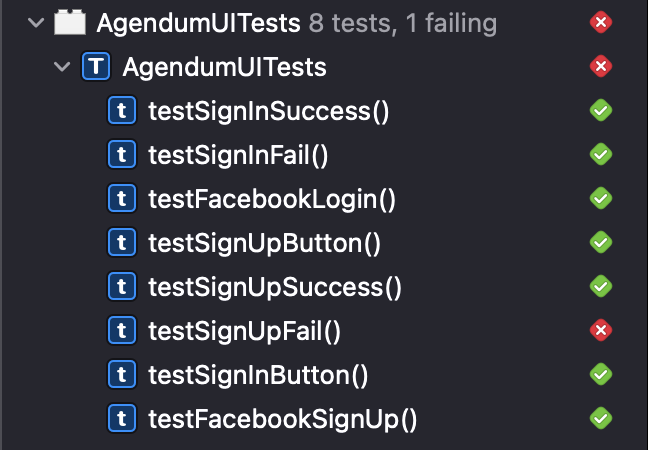
\includegraphics[width=8cm]{./graphics/testing/test results.png}
    \caption{Results from running the UI test suite.}
    \label{fig:ui_test_results}
\end{figure}
    
    As seen from the figure, the testSignUpFail UI test failed, and this is because the create account button cannot be found in the view when the test is running.  This seems to be an error in how the automation was set up rather than an error with the application itself and therefore does not leave a bug that needs to be fixed within the application.  The rest of the tests were successful; the code behind these tests can be found in the appendix under Section~\ref{app:testing_backend}.
    
    \subsection{User testing}
    Unfortunately, due to various complications during the project's implementation, there was no time to send the application out to users to be tested.  However, if this were to go ahead, the application would have been sent to a small group of users with a range of different backgrounds, including students, full-time workers and people of different age groups, to ensure the testing results would be as unbiased as possible at this stage.  A questionnaire would have also been sent out with the application with questions about the application's various features, ease of use, usefulness, and whether any bugs were encountered during the test run.  The questionnaires' results would have then been analysed, and bug fixes and improvements would have been made to the application ready for the second round of user testing.

\chapter{Reflection}
    \label{chap:reflection}
    In this chapter, what went well and what could have been improved in the project will be discussed.  Section~\ref{sec:reflection_risk} will reflect whether any of the risks defined during the risk analysis arose, as well as any unplanned risks.  Section~\ref{sec:reflection_project} will reflect on the project as a whole.
    
    \section{Risk Reflection}
    \label{sec:reflection_risk}
        During the project, some of the risks defined in the risk analysis arose.  The project's testing phase was unable to be completed in time due to unforeseen circumstances manifesting during the implementation phase.  These circumstances included the device used for development failing and needing to be sent for repair and specific tasks in the implementation stage taking longer than expected.  To mitigate the above risk, frequent sprint reviews were scheduled to ensure these events were dealt with appropriately; in the case that tasks were taking longer than expected, it was decided to continue with these as needed, and that getting the application to a working but untested condition was more critical for the project.  As for the hardware failure, while the device was sent for repair, a replacement device was used temporarily, which slowed down development during the repair period, but it was not stopped completely.
        
        There was a risk that was unplanned during the project; this was the worldwide COVID-19 pandemic.  Fortunately, the pandemic did not affect any phases of the project. It possibly would have only affected the testing phase as physically meeting with test users would not have been possible in the traditional way.  Social distancing would have had to be enforced, and masks would have needed to be worn.  However, the time frame of the project would have remained consistent with the original plan.
        
    \section{Project Reflection}
    \label{sec:reflection_project}
        Overall, the project mostly went as planned, and the application produced is satisfactory.  Due to the testing phase remaining incomplete, the final product inevitably has many bugs, and due to this, the application's behaviour may be inconsistent. However, the features defined in the requirements analysis are all present, and the basic functionality of these features is in place.
        
        If there was an opportunity to redo the project, there are some changes that would be made.  Firstly, an extensive testing plan would be designed and implemented.  The tests would contain assertion checks for how Firebase responds to requests from the application and tests to ensure that data is passed from each view within the application correctly.  More in-depth diagrams representing the flow of data between the application and the database would be produced, particularly in the context of the database.  The application designs would also conform to iOS standards more, and the fonts and colours would be consistent with the traditional iOS design.
        
        Secondly, more code-base refactoring cycles would have taken place during the implementation phase.  More time for refactoring would make the code easier to read by others and optimise the running of the application.
        
        Finally, more time would be dedicated to the testing phase.  This would allow for user testing and enough time to create all the UI and unit tests.  Having enough time for the testing phase would drastically reduce bugs and issues within the application and bring the application a step closer to being the standard it needs to be in order to be added to the App Store.

\chapter{Conclusion and Future Work}
    \label{chap:conclusion}

    \section{Future Work}
    \label{sec:conclusion_future_work}
        In this section, the future work that could be done for this project will be outlined.  
    
        Application improvements could include adding Siri integration so that users can ask Siri to add an item to the application.  Support for widgets (which was introduced in iOS14) could also be added so items could be added to the application without needing to open it.  Apple Watch support could also be added so that the users' mobile device does not need to be in use at all in order to view, add and complete items.  In terms of existing features, the 'friends' view could be improved by adding messaging support and adding the recent activity feature that initially was planned in the requirements and design.
    
        The application could also be replicated as an Android application to support more mobile devices to increase universal support.
    
    \section{Conclusion}
    \label{sec:conclusion_conclusion}
        This project's objective was to create a productivity and time management application that would help users manage their tasks throughout their day, week and month, and encourage them to be more productive and deliberate with their time.  The application that has been produced meets these requirements; users can add items that can be set as habits, tasks, events, reminders or all of the above.  They have suggested tasks based on their day's schedule.  Users can view items in their native iOS calendar and use the application to set a focus timer.  Finally, users can connect with others and use other people's progress as motivation to complete their tasks.  The application is also entirely available for free and will remain free, and has much potential for more productivity features to be added over time, outlined in Section~\ref{sec:conclusion_future_work}.
\newpage
\bibintoc
\bibliography{citations} 
\appendix
\addappheadtotoc
\chapter{Software Development Life Cycle}
    \section{Work Schedule}
    \label{app:gantt_chart}
    \begin{figure}[H]

	\centering
	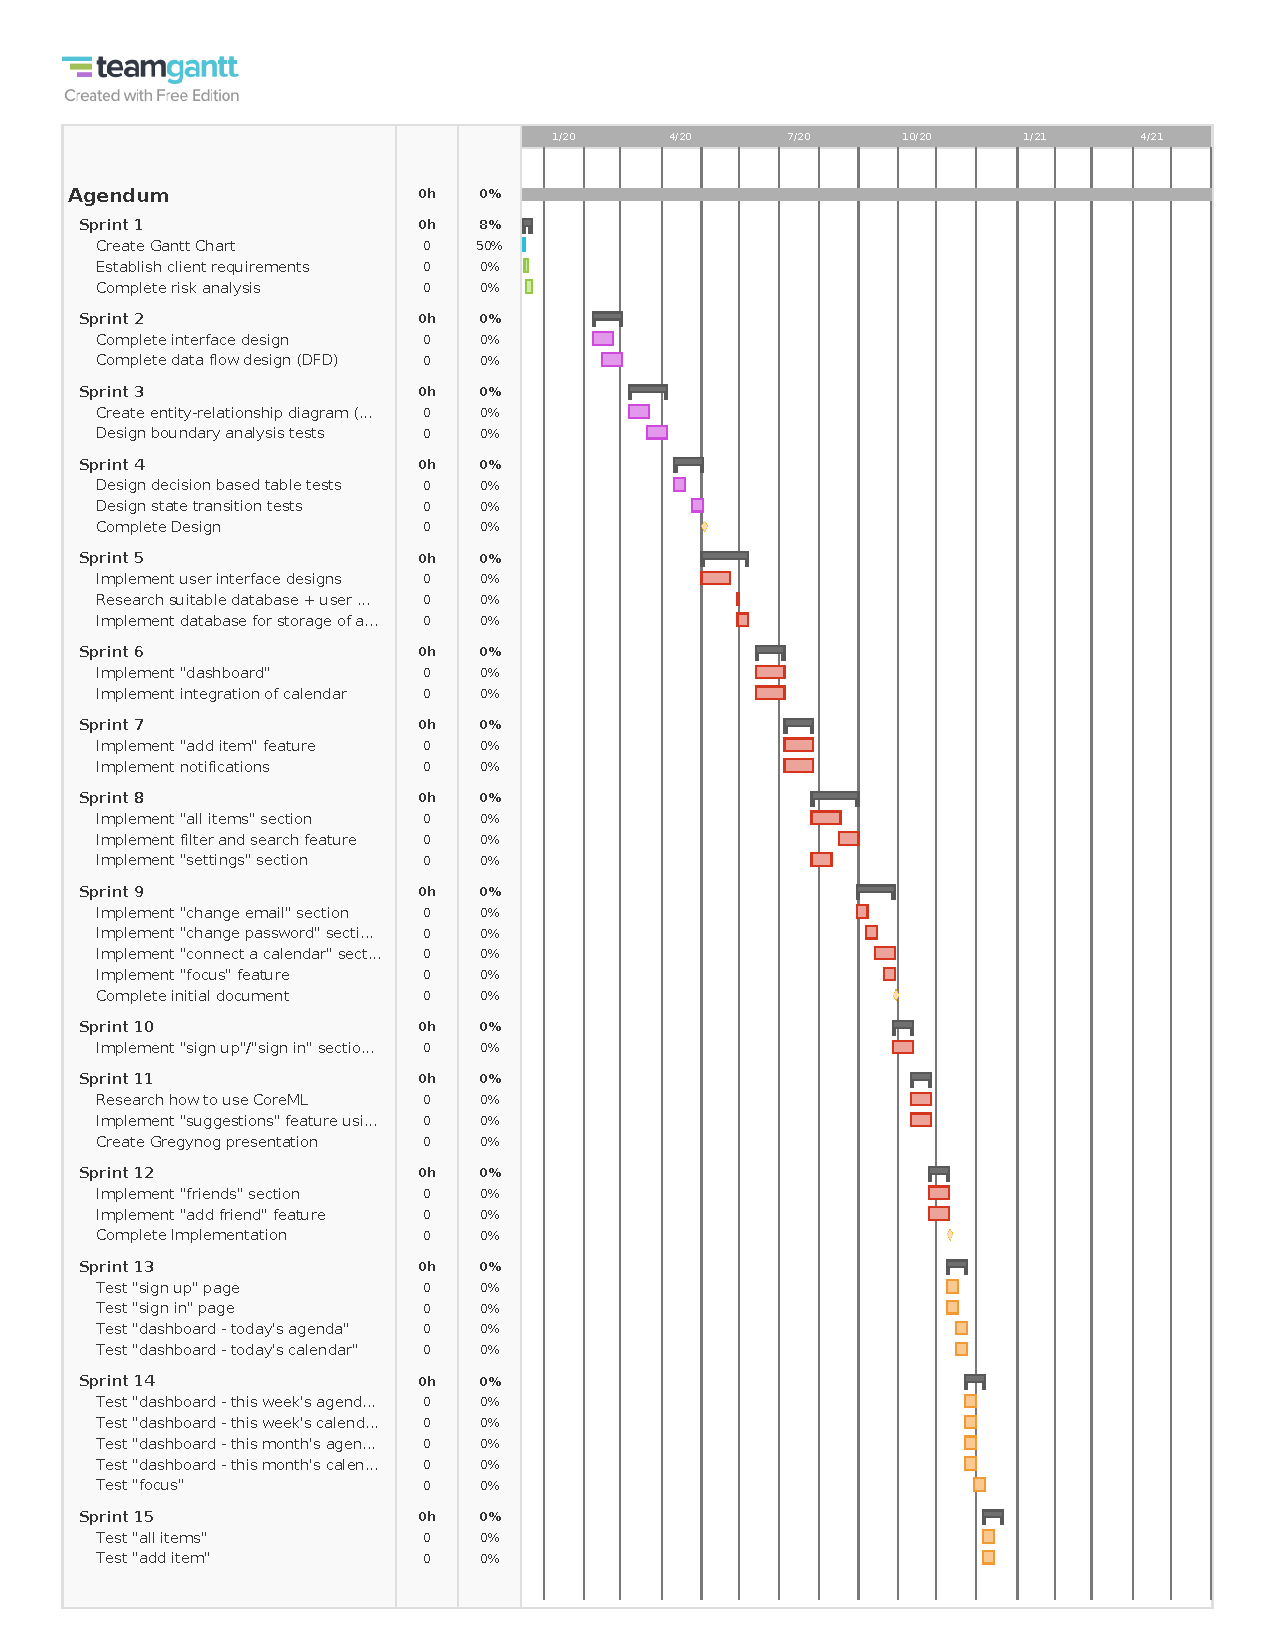
\includegraphics[width=12cm]{./graphics/gantt.pdf}
	\caption{An image of the gantt chart generated before application implementation.}
	\label{fig:gantt}
	
\end{figure}
    
    \section{Risk Analysis}
    \label{app::risk_table}
    \begin{table}[H]
\centering
\caption{Table showing risks defined at the beginning of the project. L=Likelihood, S=Severity and I=Impact.}
    \begin{tabular}{|p{5cm}|p{0.5cm}|p{0.5cm}|p{0.5cm}|p{5cm}|}
        \hline
        Risk& L& S& I& Mitigation\\
        \hline
        The requirements and design may need to be revisited and add to or changed due to unanticipated features or complexity (i.e. Gold Plating).& 4& 4& 16& Issues will be identified in sprint reviews, and extra time has been added into the schedule to accommodate these changes.\\
        \hline
        Being unable to complete tasks in the time frame specified. This could be due to unforeseen circumstances such as illness or holiday, or a task being more complex than initially expected, therefore taking longer to complete.& 4& 3& 12& Frequent sprint reviews are scheduled to ensure any incomplete tasks are appropriately dealt with and any issues are caught early on so that maximum time is given to resolve those issues.\\
        \hline
        Due to tests failing, the time period in which testing will be undertaken may be larger than expected. This will be due to having to amend code and then rerun tests until the desired outcome is achieved.& 5& 2& 10& Extra time in the work schedule has been allocated, and software will be developed with extensive validation to minimise this case.\\
        \hline
        Hardware failure may occur during the project. This can include the computer that the application is being implemented on as well as the test mobile device breaking. The computer failing will mean that development cannot continue, and the mobile device failing will mean that the application can only test on an emulator, which is not the worst-case scenario, but it means testing will not be done in a ‘real world’ environment.& 1& 5& 5& If needed, a new computer would be purchased, and the mobile device is currently under warranty and so could be replaced if damaged. Testing can also be done using an emulator.\\
        \hline
        Third-party libraries are likely to be used in the project, however at this point it is unclear exactly of what those libraries will be. As with any third-party software, there could be bugs and mistakes in those libraries which would result in errors within the application software.& 1& 2& 2&  A bug report would be sent to the developer of the library and then an alternative library to use would be found as there are usually a range of libraries to choose from that perform a similar purpose.\\
        \hline
    \end{tabular}
\end{table}
    
\chapter{Deliverables}
    \section{Requirements Analysis}
    \label{app::questionnaire}
    \begin{figure}[H]
	\centering
	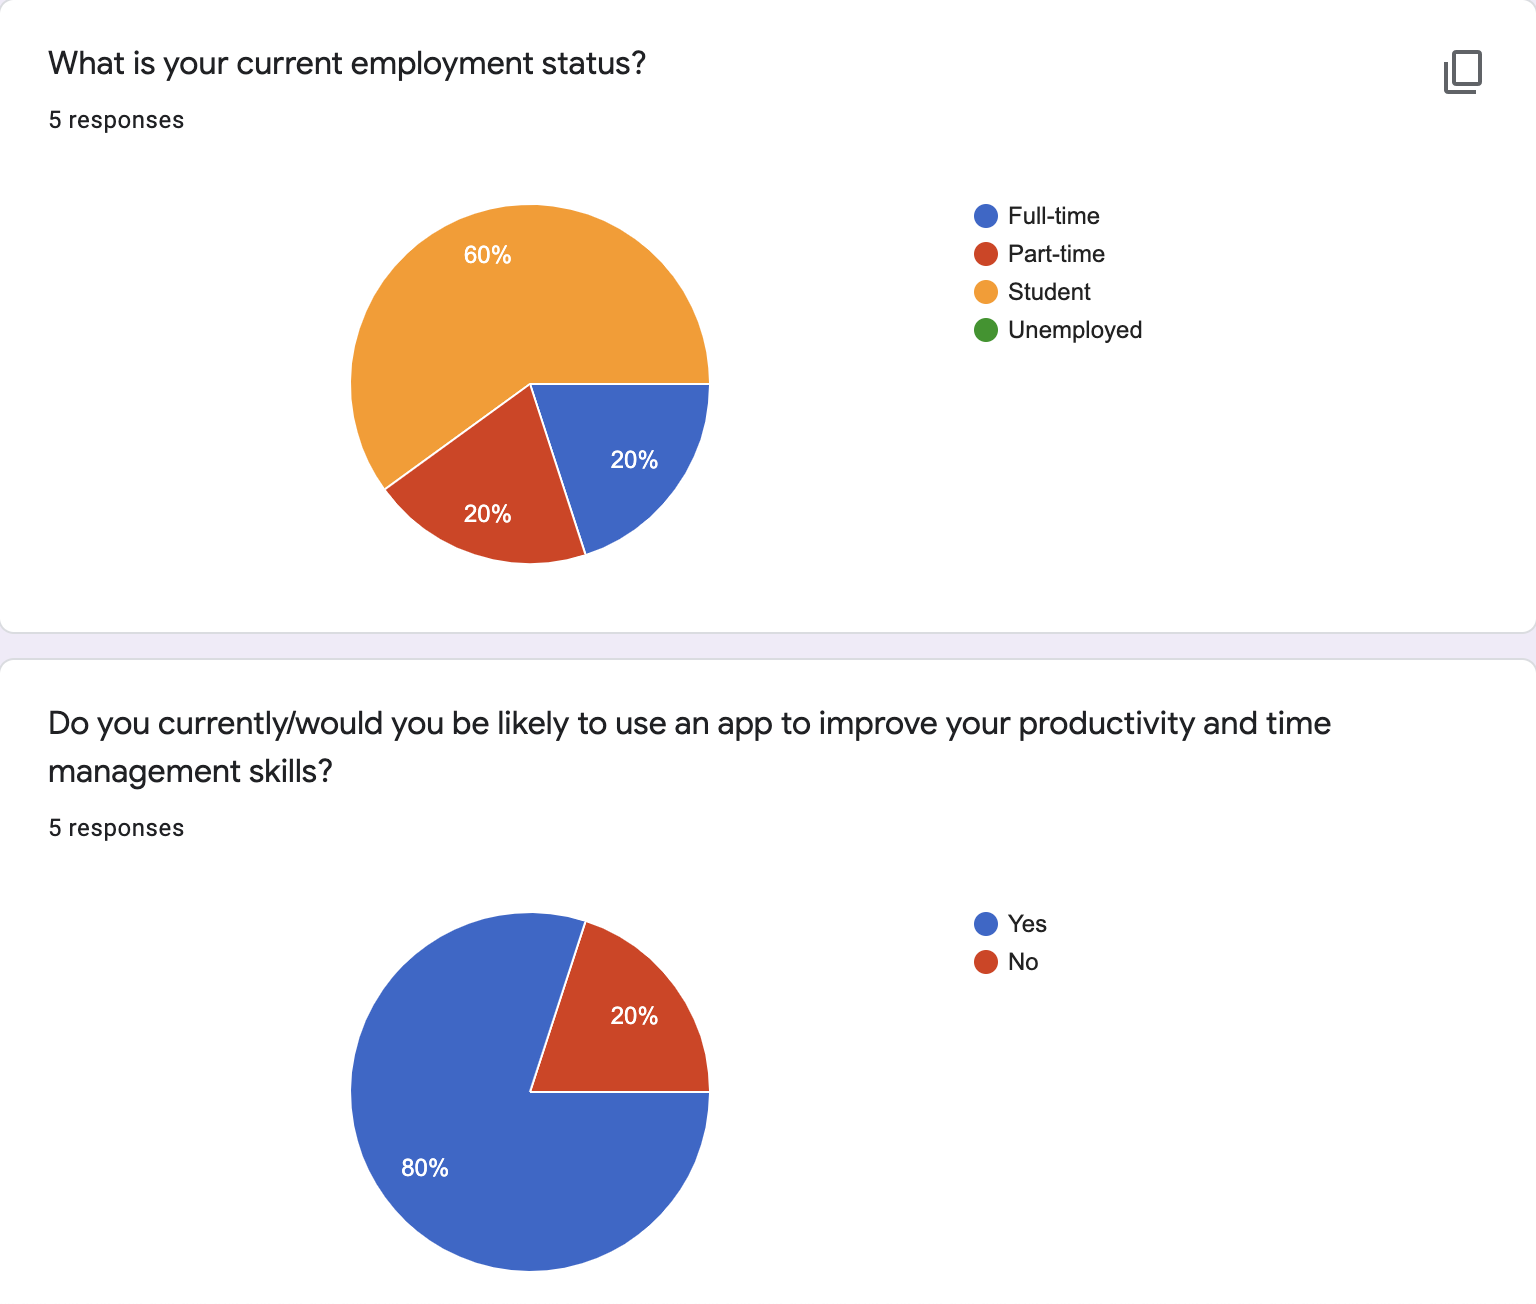
\includegraphics[width=12cm]{./graphics/questionnaire1.png}
\end{figure}

\begin{figure}[H]
    \centering
    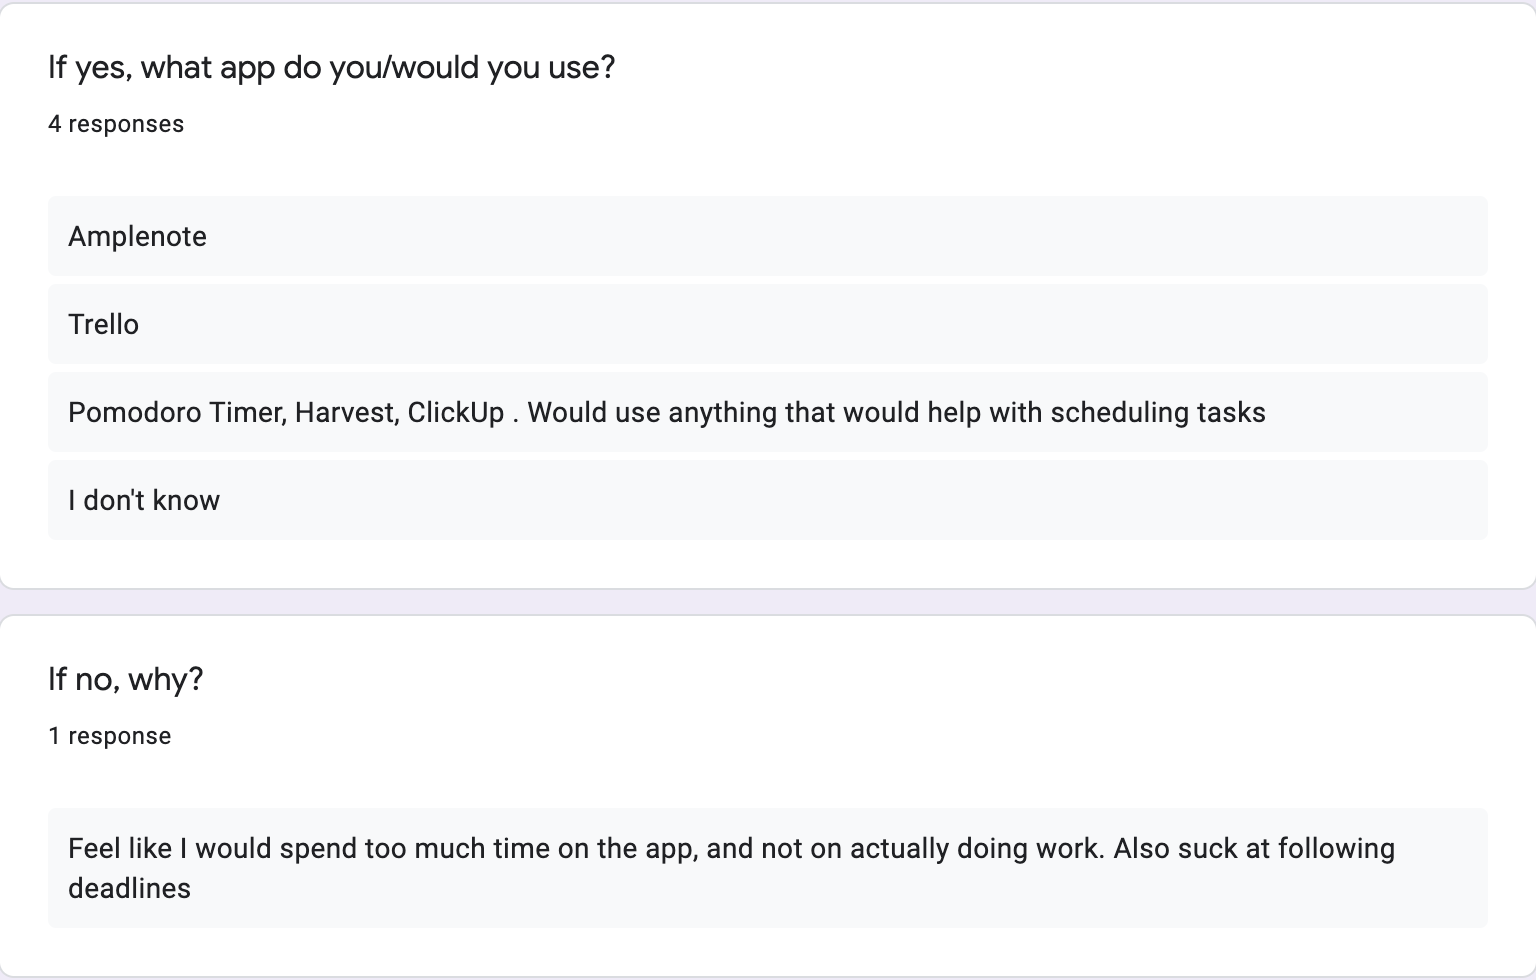
\includegraphics[width=12cm]{./graphics/questionnaire2.png}
	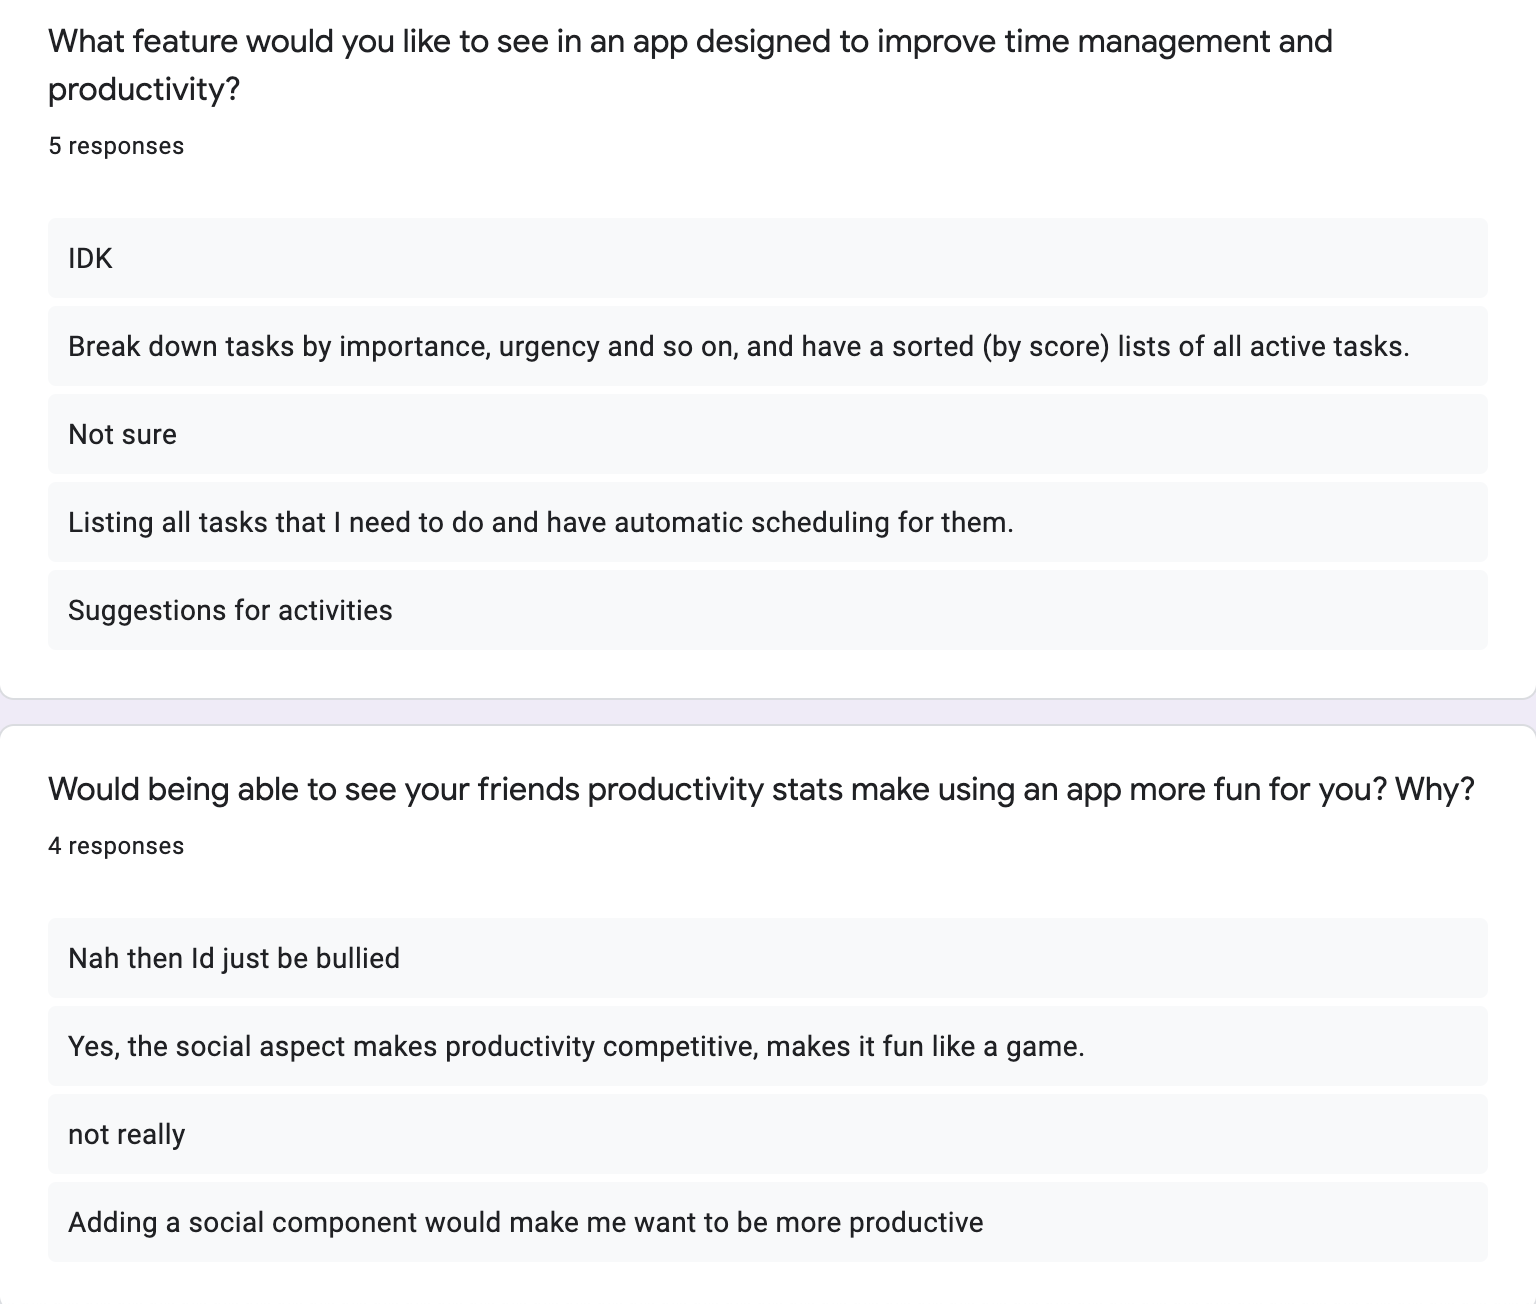
\includegraphics[width=12cm]{./graphics/questionnaire3.png}
\end{figure}

\begin{figure}[H]
    \centering
    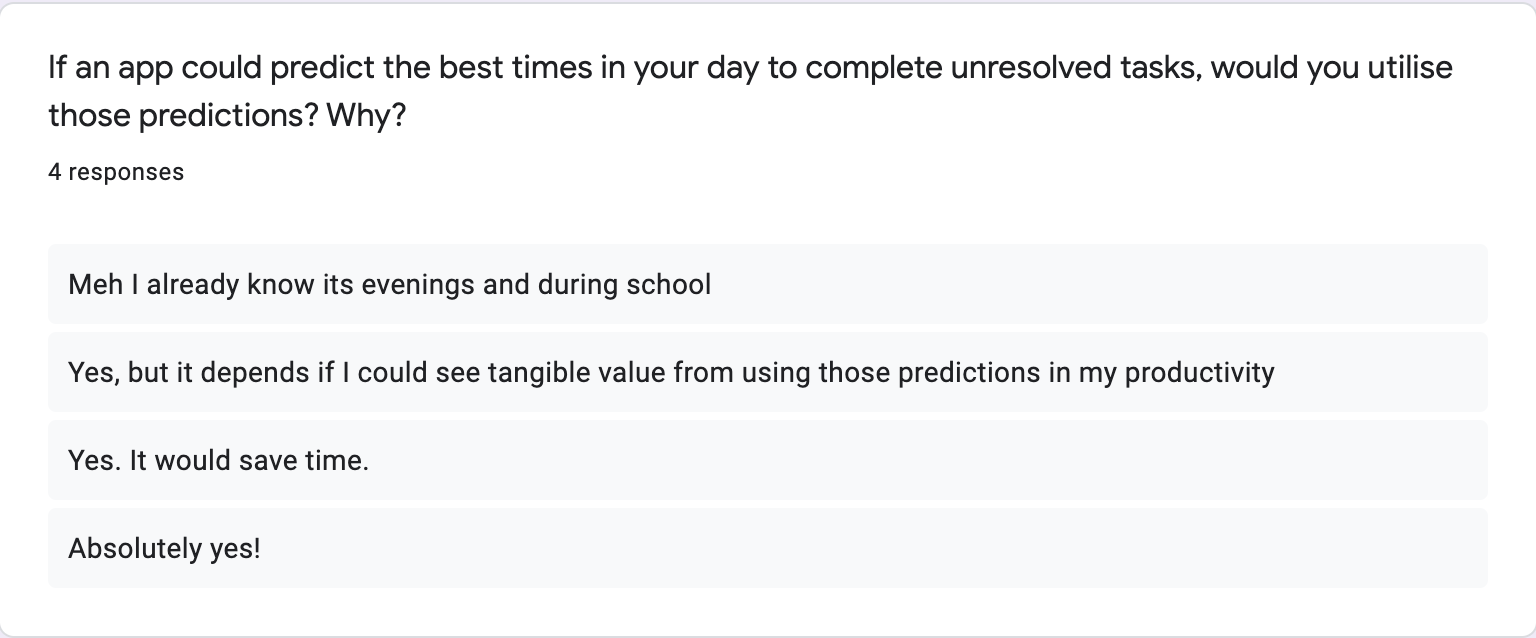
\includegraphics[width=12cm]{./graphics/questionnaire4.png}
    \caption{An image of the results of the questionnaire I conducted using Google Forms.}
	\label{fig:questionnaire}
\end{figure}
    
    \label{app::requirements_table}
    \begin{table}[H]
    \centering
    \caption{Table defining the revised functional and non-functional requirements.}
    \begin{tabular}{|p{7cm}|p{7cm}|}
        \hline
        Functional& Non-functional\\
        \hline
        The user shall have the option to sign in with either email or Facebook.& The application shall do this by displaying "Login with Facebook" as a button and an email and password text field on the sign in page.\\
        \hline
        The user shall have the option to sign up with either email or Facebook.& The application shall do this by displaying "Sign up with Facebook" as a button and an email and password text field on the sign up page.\\
        \hline
        The user shall have the option to reset their password if they are unable to sign in.& The application shall do this by displaying a clickable button that takes the user to the reset password process.\\
        \hline
        The application shall display the title screen on application start up.&\\
        \hline
        The application shall display dashboard as default screen on application start up.&\\
        \hline
        The application shall display events, tasks, reminders and suggestions relevant to the time frame option selected in the dashboard (today, this week, this month).& The application shall do this by allowing the user to swipe left or right on the time frame displayed in the dashboard to change the time frame displayed.\\
        \hline
        The user shall be able to keep track of their streak count everytime they complete an item.& The application shall do this by adding points to the streak counter displayed on the dashboard.\\
        \hline
        The user shall be able to add an item to their agenda.& The application shall do this by displaying an "add" button on the dashboard, and navigating the user to the relevant screen when that button is tapped.\\
        \hline
        The user shall be able to switch between the agenda view and the calendar view when viewing the dashboard.& The application shall do this by allowing the user to swipe left or right on the view displayed in the dashboard to switch between agenda view and calendar view.\\
        \hline
    \end{tabular}
\end{table}
    
\begin{table}[H]
    \centering
    \begin{tabular}{|p{7cm}|p{7cm}|}
        \hline
        Functional& Non-functional\\
        \hline
        The user shall be able to view their items in the calendar view in the dashboard.&  The application shall do this by displaying the items in the correct times or dates when the calendar view is in the foreground.\\
        \hline
        The user shall be able to use the focus feature within the application.& The application shall provide this by displaying the focus button within the navigation bar, and taking the user to the focus screen when it is tapped.\\
        \hline
        The user shall be able to start and stop the focus timer.&  The application shall provide this by displaying a start and stop button within the focus view.\\
        \hline
        The user shall be able to amend the focus timer settings within the focus view.& The application shall do this by allowing allowing swipe left functionality and then displaying the timer settings.\\
        \hline
        The user shall be able to view all outstanding items that have been input into the application.& The application shall do this by displaying all items when the all items button displayed in the navigation bar is tapped.\\
        \hline
        The user shall be able to view items that are due soon, items that are considered habits and labelled items as well as the rest of the added items in the all items screen.& The application shall do this by grouping items based on their theme.\\
        \hline
        The user shall be able to search for items.& The application shall do this by displaying a filter button, which when tapped, displays a search bar, and then filtering items based on the user input.\\
        \hline
        The user shall be able to edit an item.&  The application shall do this by taking the user to the edit item view when the user taps on the item.\\
        \hline
        The user shall be able to delete an item.& The application shall do this by allowing the user to swipe any direction on an item and then removing the item from being displayed, as well as deleting it from the database.\\
        \hline
        The user shall be able to navigate to the add item screen.& The application shall do this by displaying an add button on the dashboard, and navigating to the add item screen when that button is tapped.\\
        \hline
        The user shall be able to add a title, date, time, reminder, reminder date, reminder time, and labels to an item, as well as having an option to add it to their native iOS calendar.& The application shall do this by displaying ways to enter this data on the add item screen.\\
        \hline
        The user shall go back to the dashboard without saving an item.& The application shall provide this by displaying a back button on the add item screen.\\
        \hline
    \end{tabular}
\end{table}

\begin{table}[H]
    \centering
    \begin{tabular}{|p{7cm}|p{7cm}|}
        \hline
        Functional& Non-functional\\
        \hline
        The user shall be able to save an item after editing has completed.& The application shall provide this by displaying a save button at the bottom of the add item screen.\\
        \hline
        The user shall go back to the dashboard after they have saved a new item.& The application shall provide this by navigating to the dashboard after the save button has been tapped.\\
        \hline
        The user shall be able to view the "friends" screen.& The application shall provide this by displaying a friends button in the navigation bar, that when tapped, displays the "friends" screen.\\
        \hline
        The user shall be able to view their list of friends along with their friends' streak points.& The application shall provide this by retrieving their friends' user data and displaying these friends in a list, with their points next to the name on the "friends" screen.\\
        \hline
        The user shall be able to view their own streak count on the "friends" screen.& The application shall display the users' streak points at the bottom of the "friends" screen.\\
        \hline
        The user shall be able to add a friend.& The application shall display an add button on the "friends" screen, that when tapped, displays a box to add a user.\\
        \hline
        The user shall be able to find a friend via email address.& The application shall search the user database using an email address, returning a user if an email address matches.\\
        \hline
        The user shall be able to view a detailed view of a friend.& The application shall display a detailed friend view when a friend is tapped.\\
        \hline
        The user shall be able to view a friends streak points and a delete option in the detailed view.& The application shall display the email of the user, their streak points, and shall display a delete button at the bottom of the screen.\\
        \hline
        The user shall be able to delete a friend.& The application shall remove a friend from the users' friend list when the delete button is tapped.\\
        \hline
        The user shall be able to go back to the "friends" screen.& The application shall display a back button the the friend detail screen, that when tapped will display the "friends" screen.\\
        \hline
        The user shall be able to go to the settings screen.& The application shall display a settings button in the navigation bar, which when tapped, shall display the settings screen.\\
        \hline
        The user shall be able to edit their email and/or password, as well as connect the native iOS calendar, delete their account and activate bio-metric authentication.& The application shall display options to change the email or password, a toggle to allow access to the iOS calendar, a delete button and a toggle to activate bio-metric authentication.\\
        \hline
        The user shall be able to delete their account.& The application shall provide a delete button, which when tapped, will remove the user account on the database along with any related information, and will then display the sign up screen.\\
        \hline
    \end{tabular}
\end{table}

\begin{table}[H]
    \centering
    \begin{tabular}{|p{7cm}|p{7cm}|}
        \hline
        Functional& Non-functional\\
        \hline
        The user shall receive notifications.& The application shall send notifications at times corresponding with the dates and times set up for reminders. (Provided the user has allowed notifications on application set-up).\\
        \hline
        & The application shall store the users' name, email and password securely in the database.\\
        \hline
        & The application shall download application data from the database when the application is opened.\\
        \hline
    \end{tabular}
\end{table}
    
    \section{Design}
    \subsection{User Interface}
    \subsubsection{Wireframes}
    \label{app::mockups}
    \begin{figure}[H]
    \centering
    \begin{subfigure}[b]{0.3\textwidth}
        \centering
        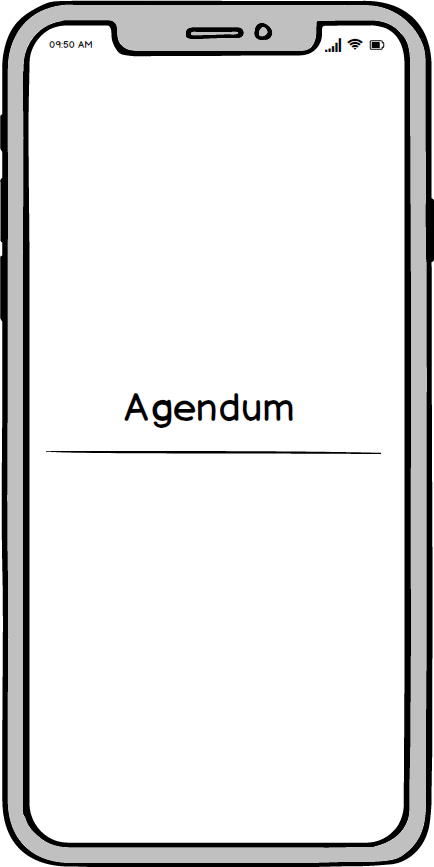
\includegraphics[width=\textwidth]{./graphics/design/Start.png}
        \caption{Splash Screen.}
        \label{fig:start}
    \end{subfigure}
    \hfill
    \begin{subfigure}[b]{0.3\textwidth}
        \centering
        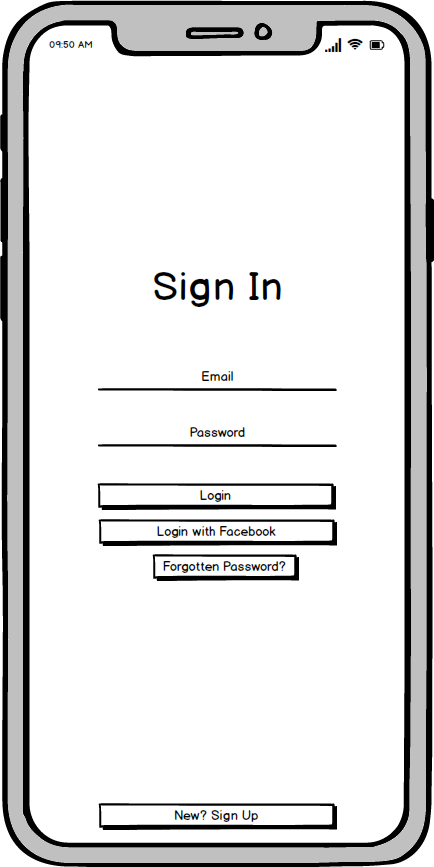
\includegraphics[width=\textwidth]{./graphics/design/Sign In.png}
        \caption{Sign In.}
        \label{fig:sign_in}
    \end{subfigure}
    \hfill
    \begin{subfigure}[b]{0.3\textwidth}
        \centering
        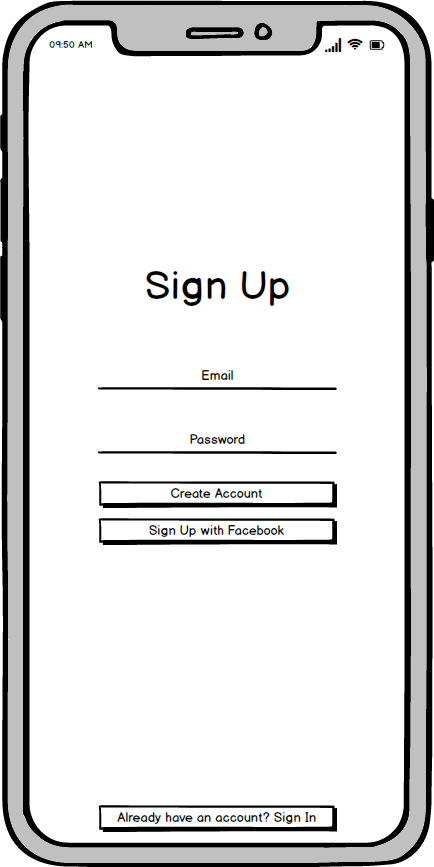
\includegraphics[width=\textwidth]{./graphics/design/Sign Up.png}
        \caption{Sign Up.}
        \label{fig:sign_up}
    \end{subfigure}
    
    \caption{Mockup designs of the splash screen, sign up and sign in views.}
    \label{fig:splash_signup_signin}
\end{figure}

\begin{figure}
    \centering
    \begin{subfigure}[b]{0.3\textwidth}
        \centering
        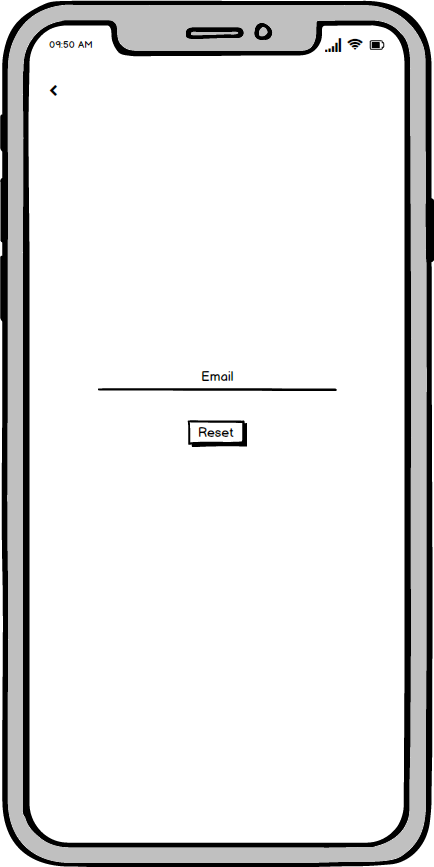
\includegraphics[width=\textwidth]{./graphics/design/Forgotten Password.png}
        \caption{Forgotten Password.}
        \label{fig:forgotten_password}
    \end{subfigure}
    \hfill
    \begin{subfigure}[b]{0.3\textwidth}
        \centering
        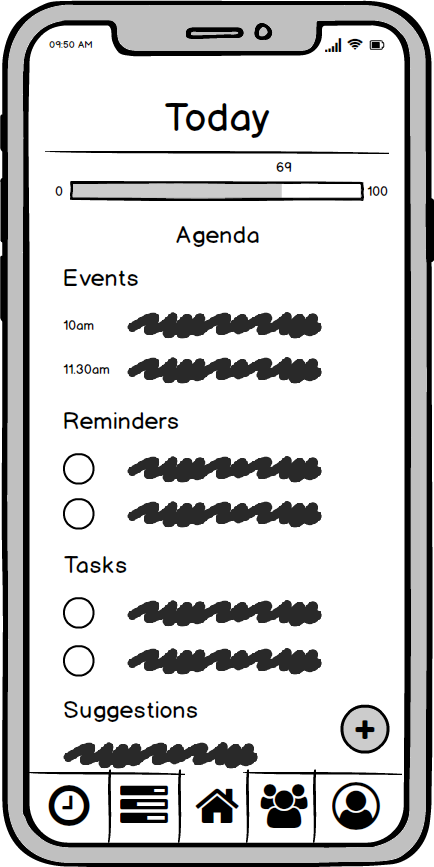
\includegraphics[width=\textwidth]{./graphics/design/Dashboard.png}
        \caption{Agenda Today.}
        \label{fig:dashboard_agenda_today}
    \end{subfigure}
    \hfill
    \begin{subfigure}[b]{0.3\textwidth}
        \centering
        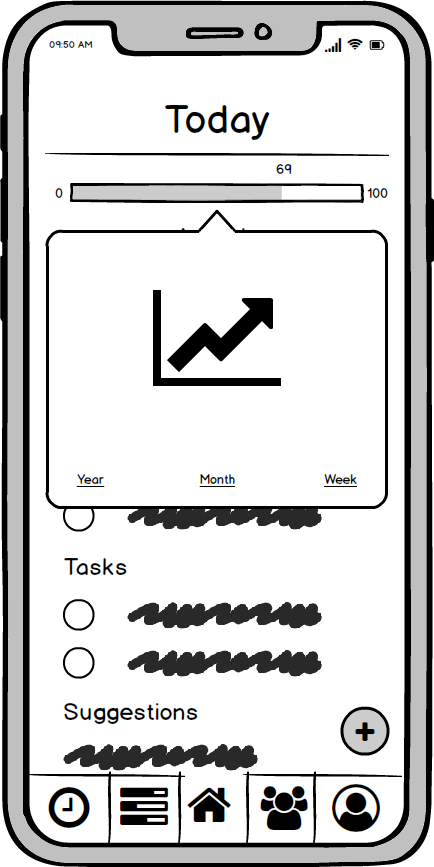
\includegraphics[width=\textwidth]{./graphics/design/Dashboard (Streak trend Agenda View).png}
        \caption{Streak Trend in Agenda View.}
        \label{fig:dashboard_streak_agenda}
    \end{subfigure}
    
    \caption{Mockup designs of the forgotten password, agenda today, and streak trend in the agenda views.}
    \label{fig:forgotten_todayagenda_agendastreak}
\end{figure}

\begin{figure}
    \centering
    \begin{subfigure}[b]{0.3\textwidth}
        \centering
        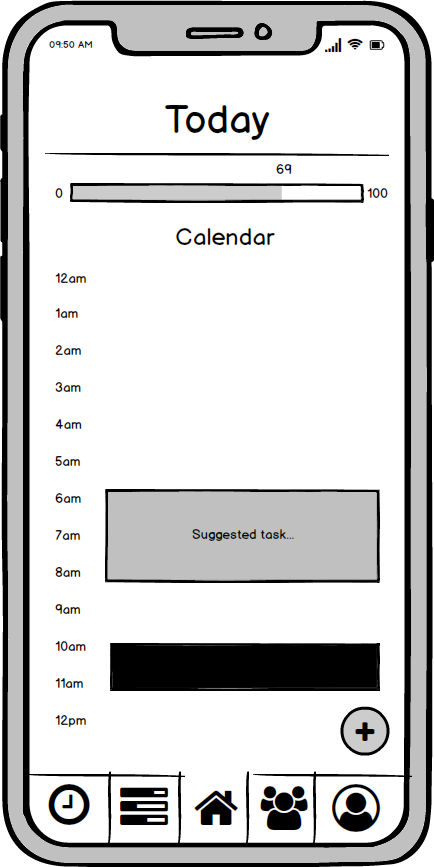
\includegraphics[width=\textwidth]{./graphics/design/Dashboard (Today Calendar View).png}
        \caption{Calendar Today.}
        \label{fig:calendar_today}
    \end{subfigure}
    \hfill
    \begin{subfigure}[b]{0.3\textwidth}
        \centering
        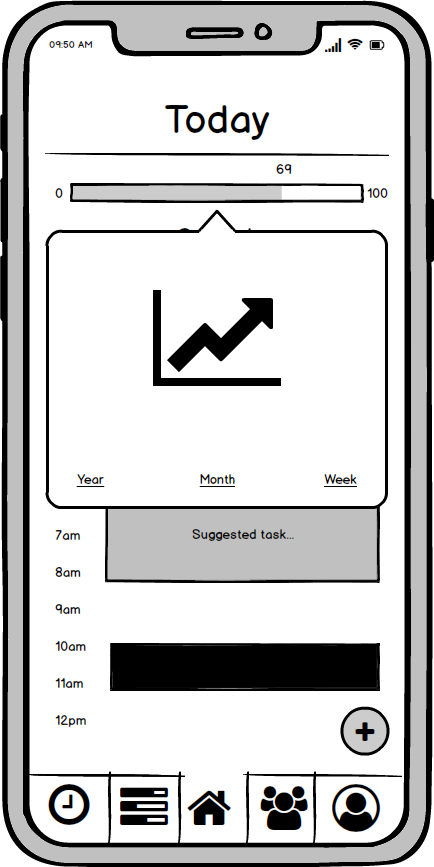
\includegraphics[width=\textwidth]{./graphics/design/Dashboard (Streak trend Calendar View).png}
        \caption{Streak trend in Calendar View.}
        \label{fig:dashboard_streak_calendar}
    \end{subfigure}
    \hfill
    \begin{subfigure}[b]{0.3\textwidth}
        \centering
        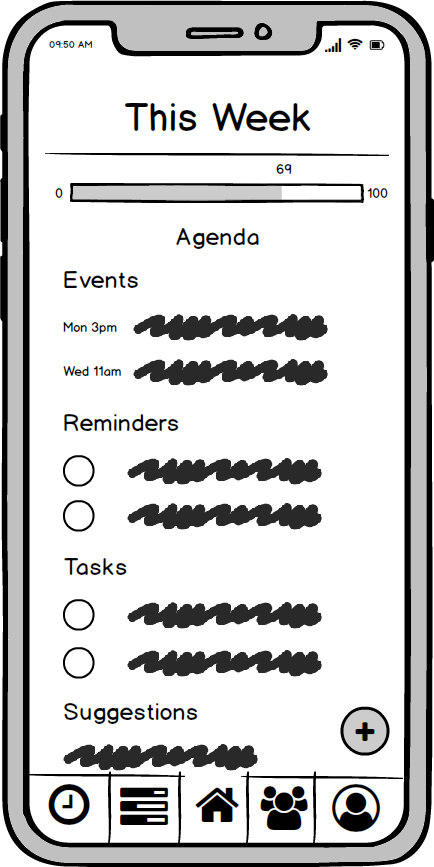
\includegraphics[width=\textwidth]{./graphics/design/Dashboard (This Week Agenda View).png}
        \caption{Agenda This Week.}
        \label{fig:this_week_agenda}
    \end{subfigure}
    
    \caption{Mockup designs of the today calendar, streak view in calendar and this week agenda views.}
    \label{fig:todaycal_streakcal_thisweekagenda}
\end{figure}

\begin{figure}
    \centering
    \begin{subfigure}[b]{0.3\textwidth}
        \centering
        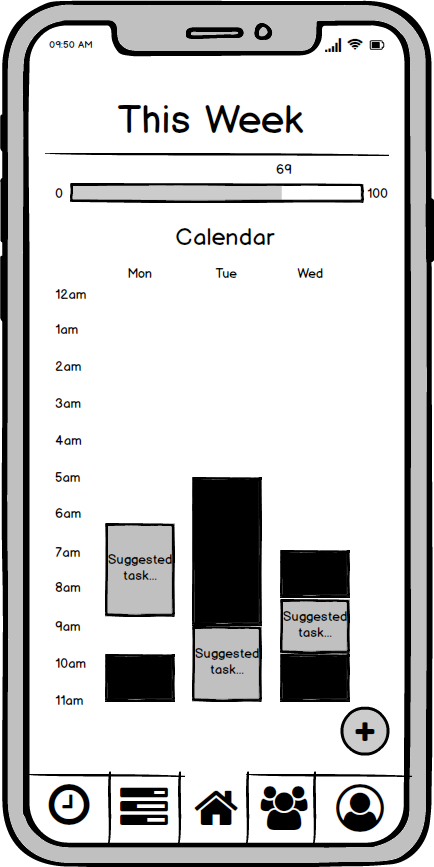
\includegraphics[width=\textwidth]{./graphics/design/Dashboard (This Week Calendar View).png}
        \caption{Calendar This Week.}
        \label{fig:calendar_this_week}
    \end{subfigure}
    \hfill
    \begin{subfigure}[b]{0.3\textwidth}
        \centering
        \includegraphics[width=\textwidth]{./graphics/design/Dashboard (This Month Agenda View).png}
        \caption{Agenda This Month.}
        \label{fig:agenda_this_month}
    \end{subfigure}
    \hfill
    \begin{subfigure}[b]{0.3\textwidth}
        \centering
        \includegraphics[width=\textwidth]{./graphics/design/Dashboard (This Month Calendar View).png}
        \caption{Calendar This Month.}
        \label{fig:this_month_calendar}
    \end{subfigure}
    
    \caption{Mockup designs of calendar this week, agenda this month and calendar this month views.}
    \label{fig:calthisweek_agendathismonth_calthismonth}
\end{figure}

\begin{figure}
    \centering
    \begin{subfigure}[b]{0.3\textwidth}
        \centering
        \includegraphics[width=\textwidth]{./graphics/design/Add item.png}
        \caption{Add Item View.}
        \label{fig:add_item}
    \end{subfigure}
    \hfill
    \begin{subfigure}[b]{0.3\textwidth}
        \centering
        \includegraphics[width=\textwidth]{./graphics/design/Focus.png}
        \caption{Focus View.}
        \label{fig:focus}
    \end{subfigure}
    \hfill
    \begin{subfigure}[b]{0.3\textwidth}
        \centering
        \includegraphics[width=\textwidth]{./graphics/design/All Items.png}
        \caption{All Items View.}
        \label{fig:all_items}
    \end{subfigure}
    
    \caption{Mockup designs of the add item, focus and all items views.}
    \label{fig:additem_focus_allitems}
\end{figure}

\begin{figure}
    \centering
    \begin{subfigure}[b]{0.3\textwidth}
        \centering
        \includegraphics[width=\textwidth]{./graphics/design/Friends.png}
        \caption{Friends View.}
        \label{fig:friends}
    \end{subfigure}
    \hfill
    \begin{subfigure}[b]{0.3\textwidth}
        \centering
        \includegraphics[width=\textwidth]{./graphics/design/Friends (Recent Activity).png}
        \caption{Friends' Recent Activity View.}
        \label{fig:friends_recent}
    \end{subfigure}
    \hfill
    \begin{subfigure}[b]{0.3\textwidth}
        \centering
        \includegraphics[width=\textwidth]{./graphics/design/User Account.png}
        \caption{Settings View.}
        \label{fig:settings}
    \end{subfigure}
    
    \caption{Mockup designs of the friends, friends' recent activity and settings views.}
    \label{fig:friends_friendsrecent_settings}
\end{figure}

\begin{figure}
    \centering
    \begin{subfigure}[b]{0.3\textwidth}
        \centering
        \includegraphics[width=\textwidth]{./graphics/design/Change Email.png}
        \caption{Change Email View.}
        \label{fig:change_email}
    \end{subfigure}
    \hfill
    \begin{subfigure}[b]{0.3\textwidth}
        \centering
        \includegraphics[width=\textwidth]{./graphics/design/Change Password.png}
        \caption{Change Password View.}
        \label{fig:change_password}
    \end{subfigure}
    \hfill
    \begin{subfigure}[b]{0.3\textwidth}
        \centering
        \includegraphics[width=\textwidth]{./graphics/design/Connect Calendar.png}
        \caption{Connect Calendar View.}
        \label{fig:connect_calendar}
    \end{subfigure}
    
    \caption{Mockup designs of the change email, change password and connect calendar views.}
    \label{fig:changeemail_changepassword_connectcalendar}
\end{figure}

\begin{figure}[H]
    \centering
    \includegraphics[width=4cm]{./graphics/design/User Account (Delete Account).png}
    \caption{Delete Account View.}
    \label{fig:delete_account}
\end{figure}
    
    \subsubsection{Colour Designs}
    \label{app:colour}
    \begin{figure}[H]
    \centering
    \begin{subfigure}[b]{0.3\textwidth}
        \centering
        \includegraphics[width=\textwidth]{./graphics/design/Start Up Colour.png}
        \caption{Splash Screen.}
        \label{fig:start_colour}
    \end{subfigure}
    \hfill
    \begin{subfigure}[b]{0.3\textwidth}
        \centering
        \includegraphics[width=\textwidth]{./graphics/design/Sign In Colour.png}
        \caption{Sign In.}
        \label{fig:sign_in_colour}
    \end{subfigure}
    \hfill
    \begin{subfigure}[b]{0.3\textwidth}
        \centering
        \includegraphics[width=\textwidth]{./graphics/design/Sign Up Colour.png}
        \caption{Sign Up.}
        \label{fig:sign_up_colour}
    \end{subfigure}
    
    \caption{Colour designs of the splash screen, sign up and sign in views.}
    \label{fig:splash_signup_signin_colour}
\end{figure}

\begin{figure}[H]
    \centering
    \begin{subfigure}[b]{0.3\textwidth}
        \centering
        \includegraphics[width=\textwidth]{./graphics/design/Sign In - Forgotten Password Colour.png}
        \caption{Forgotten Password View.}
        \label{fig:forgotten_password_colour}
    \end{subfigure}
    \hfill
    \begin{subfigure}[b]{0.3\textwidth}
        \centering
        \includegraphics[width=\textwidth]{./graphics/design/Dashboard - Agenda View - Today.png}
        \caption{Agenda Today View.}
        \label{fig:agenda_today_colour}
    \end{subfigure}
    \hfill
    \begin{subfigure}[b]{0.3\textwidth}
        \centering
        \includegraphics[width=\textwidth]{./graphics/design/Dashboard - Calendar View - Today.png}
        \caption{Calendar Today View}
        \label{fig:calendar_today_colour}
    \end{subfigure}
    
    \caption{Colour designs of the forgotten password, agenda today and calendar today views.}
    \label{fig:forgottenpassword_agendatoday_calendartoday_colour}
\end{figure}

\begin{figure}[H]
    \centering
    \begin{subfigure}[b]{0.3\textwidth}
        \centering
        \includegraphics[width=\textwidth]{./graphics/design/Dashboard - Agenda View - This Week.png}
        \caption{Agenda This Week View.}
        \label{fig:agenda_this_week_colour}
    \end{subfigure}
    \hfill
    \begin{subfigure}[b]{0.3\textwidth}
        \centering
        \includegraphics[width=\textwidth]{./graphics/design/Dashboard - Calendar View - This Week.png}
        \caption{Calendar This Week View.}
        \label{fig:calendar_this_week_colour}
    \end{subfigure}
    \hfill
    \begin{subfigure}[b]{0.3\textwidth}
        \centering
        \includegraphics[width=\textwidth]{./graphics/design/Dashboard - Agenda View - This Month.png}
        \caption{Agenda This Month View.}
        \label{fig:agenda_this_month_colour}
    \end{subfigure}
    
    \caption{Colour designs of the agenda this week, calendar this week and agenda this month views.}
    \label{fig:agendathisweek_calthisweek_agendathismonth_colour}
\end{figure}

\begin{figure}[H]
    \centering
    \begin{subfigure}[b]{0.3\textwidth}
        \centering
        \includegraphics[width=\textwidth]{./graphics/design/Dashboard - Calendar View - This Month.png}
        \caption{Calendar This Month View.}
        \label{fig:calendar_this_month_colour}
    \end{subfigure}
    \hfill
    \begin{subfigure}[b]{0.3\textwidth}
        \centering
        \includegraphics[width=\textwidth]{./graphics/design/Focus Colour.png}
        \caption{Focus View.}
        \label{fig:focus_colour}
    \end{subfigure}
    \hfill
    \begin{subfigure}[b]{0.3\textwidth}
        \centering
        \includegraphics[width=\textwidth]{./graphics/design/Focus Settings Colour.png}
        \caption{Focus Settings View.}
        \label{fig:focus_settings_colour}
    \end{subfigure}
    
    \caption{Colour designs of the calendar this month, focus and focus settings views.}
    \label{fig:calthismonth_focus_focussettings_colour}
\end{figure}

\begin{figure}[H]
    \centering
    \begin{subfigure}[b]{0.3\textwidth}
        \centering
        \includegraphics[width=\textwidth]{./graphics/design/Add Item Colour.png}
        \caption{Add Item View.}
        \label{fig:add_item_colour}
    \end{subfigure}
    \hfill
    \begin{subfigure}[b]{0.3\textwidth}
        \centering
        \includegraphics[width=\textwidth]{./graphics/design/All Items Colour.png}
        \caption{All Items View.}
        \label{fig:all_items_colour}
    \end{subfigure}
    \hfill
    \begin{subfigure}[b]{0.3\textwidth}
        \centering
        \includegraphics[width=\textwidth]{./graphics/design/Friends Colour.png}
        \caption{Friends View.}
        \label{fig:friends_colour}
    \end{subfigure}
    
    \caption{Colour designs of the add item, all items and friends views.}
    \label{fig:additem_allitems_friends_colour}
\end{figure}

\begin{figure}[H]
    \centering
    \begin{subfigure}[b]{0.3\textwidth}
        \centering
        \includegraphics[width=\textwidth]{./graphics/design/Friends - Recent Activity.png}
        \caption{Friends' Recent Activity View.}
        \label{fig:friends_recent_colour}
    \end{subfigure}
    \hfill
    \begin{subfigure}[b]{0.3\textwidth}
        \centering
        \includegraphics[width=\textwidth]{./graphics/design/Settings Colour.png}
        \caption{Settings View.}
        \label{fig:settings_colour}
    \end{subfigure}
    
    \caption{Colour designs of the friends recent activity and settings views.}
    \label{fig:friendsrecent_settings_colour}
\end{figure}
    
    \subsubsection{Data Flow Diagrams}
    \label{app:dfd}
    \begin{figure}[H]

	\centering
	\includegraphics[width=8cm]{./graphics/design/DFD/Sign In + Sign Up DFD.png}
	\caption{The DFD for the sign in and sign up views.}
	\label{fig:signin_signup_dfd}
	
\end{figure}

\begin{figure}[H]

	\centering
	\includegraphics[width=8cm]{./graphics/design/DFD/Dashboard + Items DFD.png}
	\caption{The DFD for the dashboard and all items view.}
	\label{fig:dashboard_allitems_dfd}
	
\end{figure}

\begin{figure}[H]

	\centering
	\includegraphics[width=8cm]{./graphics/design/DFD/Focus DFD.png}
	\caption{The DFD for the focus view.}
	\label{fig:focus_dfd}
	
\end{figure}

\begin{figure}[H]

	\centering
	\includegraphics[width=8cm]{./graphics/design/DFD/Friends DFD.png}
	\caption{The DFD for the friends view.}
	\label{fig:friends_dfd}
	
\end{figure}
    
    \subsubsection{Entity-Relationship Diagram}
    \label{app:er}
    \begin{figure}[H]

	\centering
	\includegraphics[width=14cm]{./graphics/design/E-R Diagram.png}
	\caption{The entity-relationship diagram produced during the design phase of the project.}
	\label{fig:er_diagram}
	
\end{figure}
    
    \section{Implementation}
    \subsection{Splash/Sign Up/Sign In}
    \subsubsection{Front-end}
    \label{app:facebook_login_frontend}
    \begin{figure}[H]
    \centering
    \begin{subfigure}[b]{0.3\textwidth}
        \centering
        \includegraphics[width=\textwidth]{./graphics/Implementation/Splash_Sign_Up_Sign_In/facebook1.png}
        \caption{Permission to login with Facebook alert.}
        \label{fig:facebook1_app}
    \end{subfigure}
    \hfill
    \begin{subfigure}[b]{0.3\textwidth}
        \centering
        \includegraphics[width=\textwidth]{./graphics/Implementation/Splash_Sign_Up_Sign_In/facebook2.png}
        \caption{Facebook Login.}
        \label{fig:facebook2_app}
    \end{subfigure}
    
    \caption{The Facebook login process from the sign up/sign in views.}
    \label{fig:facebook_login_app}
\end{figure}
    \subsubsection{Back-end}
    \label{app:splash_signup_signin_backend}
    \begin{figure}[H]
    \centering
    \includegraphics[width=\textwidth]{./graphics/Implementation/Add Item/notifications1.png}
    \caption{requestPermissions() function in the Notifications class.}
    \label{fig:notifications1}
\end{figure}

\begin{figure}[H]
    \centering
    \includegraphics[width=\textwidth]{./graphics/Implementation/Add Item/notifications2.png}
    \caption{generateNotification() function in the Notifications class.}
    \label{fig:notifications2}
\end{figure}
    
    \subsection{Dashboard}
    \subsubsection{Back-end}
    \label{app:dashboard_backend}
    \begin{figure}[H]
    \centering
    \includegraphics[width=\textwidth]{./graphics/Implementation/Dashboard/firebasesession1.png}
    \caption{deleteItem() function defined in FirebaseSession class.}
    \label{fig:firebasesession1_dashboard}
\end{figure}

\begin{figure}[H]
    \centering
    \includegraphics[width=\textwidth]{./graphics/Implementation/Dashboard/firebasesession2.png}
    \caption{saveItem() function defined in FirebaseSession class.}
    \label{fig:firebasesession2_dashboard}
\end{figure}

\begin{figure}[H]
    \centering
    \includegraphics[width=\textwidth]{./graphics/Implementation/Dashboard/firebasesession3.png}
    \caption{saveItems() function defined in FirebaseSession class.}
    \label{fig:firebasesession3_dashboard}
\end{figure}

\begin{figure}[H]
    \centering
    \includegraphics[width=\textwidth]{./graphics/Implementation/Dashboard/firebasesession4.png}
    \caption{retrieveProgress() function defined in FirebaseSession class.}
    \label{fig:firebasesession4_dashboard}
\end{figure}

\begin{figure}[H]
    \centering
    \includegraphics[width=\textwidth]{./graphics/Implementation/Dashboard/firebasesession5.png}
    \caption{saveProgress() function defined in FirebaseSession class.}
    \label{fig:firebasesession5_dashboard}
\end{figure}

\begin{figure}[H]
    \centering
    \includegraphics[width=\textwidth]{./graphics/Implementation/Dashboard/firebasesession6.png}
    \caption{retrieveLabels() and saveLabels() functions defined in FirebaseSession class.}
    \label{fig:firebasesession6_dashboard}
\end{figure}

\begin{figure}[H]
    \centering
    \includegraphics[width=\textwidth]{./graphics/Implementation/Dashboard/firebasesession7.png}
    \caption{retrieveItems() function defined in FirebaseSession class.}
    \label{fig:firebasesession7_dashboard}
\end{figure}

\begin{figure}[H]
    \centering
    \includegraphics[width=\textwidth]{./graphics/Implementation/Dashboard/item1.png}
    \caption{public variables and constructors defined in Item class.}
    \label{fig:item1}
\end{figure}

\begin{figure}[H]
    \centering
    \includegraphics[width=9cm]{./graphics/Implementation/Dashboard/item2.png}
    \caption{Getter and Setter functions defined in Item class.}
    \label{fig:item2}
\end{figure}

\begin{figure}[H]
    \centering
    \includegraphics[width=\textwidth]{./graphics/Implementation/Dashboard/item3.png}
    \caption{Getter and Setter functions defined in Item class.}
    \label{fig:item3}
\end{figure}

\begin{figure}[H]
    \centering
    \includegraphics[width=\textwidth]{./graphics/Implementation/Dashboard/item4.png}
    \caption{Getter and Setter functions defined in Item class.}
    \label{fig:item4}
\end{figure}
    
    \subsection{Add Item}
    \subsubsection{Back-end}
    \label{app:add_item_backend}
    \begin{figure}[H]
    \centering
    \includegraphics[width=\textwidth]{./graphics/Implementation/Add Item/notifications1.png}
    \caption{requestPermissions() function in the Notifications class.}
    \label{fig:notifications1}
\end{figure}

\begin{figure}[H]
    \centering
    \includegraphics[width=\textwidth]{./graphics/Implementation/Add Item/notifications2.png}
    \caption{generateNotification() function in the Notifications class.}
    \label{fig:notifications2}
\end{figure}
    
    \subsection{Friends}
    \subsubsection{Back-end}
    \label{app:friends_backend}
    \begin{figure}[H]
    \centering
    \includegraphics[width=\textwidth]{./graphics/Implementation/Add Item/notifications1.png}
    \caption{requestPermissions() function in the Notifications class.}
    \label{fig:notifications1}
\end{figure}

\begin{figure}[H]
    \centering
    \includegraphics[width=\textwidth]{./graphics/Implementation/Add Item/notifications2.png}
    \caption{generateNotification() function in the Notifications class.}
    \label{fig:notifications2}
\end{figure}
    
    \subsection{Settings}
    \subsubsection{Front-end}
    \label{app:settings_frontend}
    \begin{figure}[H]
    \centering
    \begin{subfigure}[b]{0.3\textwidth}
        \centering
        \includegraphics[width=\textwidth]{./graphics/Implementation/Settings/change password.png}
        \caption{Change Password pop-up.}
        \label{fig:change_password_app}
    \end{subfigure}
    \hfill
    \begin{subfigure}[b]{0.3\textwidth}
        \centering
        \includegraphics[width=\textwidth]{./graphics/Implementation/Settings/faceid.png}
        \caption{Face ID activation.}
        \label{fig:faceid_app}
    \end{subfigure}
    
    \caption{Change Password pop-up and Face ID activation.}
    \label{fig:change_password_faceid}
\end{figure}
    \subsubsection{Back-end}
    \begin{figure}[H]
    \centering
    \includegraphics[width=\textwidth]{./graphics/Implementation/Add Item/notifications1.png}
    \caption{requestPermissions() function in the Notifications class.}
    \label{fig:notifications1}
\end{figure}

\begin{figure}[H]
    \centering
    \includegraphics[width=\textwidth]{./graphics/Implementation/Add Item/notifications2.png}
    \caption{generateNotification() function in the Notifications class.}
    \label{fig:notifications2}
\end{figure}
    
    \section{Testing}
    \subsubsection{UI Tests}
    \label{app:testing_backend}
    \begin{figure}[H]
    \centering
    \includegraphics[width=\textwidth]{./graphics/testing/testing1.png}
    \caption{testSignInSuccess() and testSignInFail() UI tests.}
    \label{fig:testing1}
\end{figure}

\begin{figure}[H]
    \centering
    \includegraphics[width=\textwidth]{./graphics/testing/testing2.png}
    \caption{testFacebookLogin() and testSignUpButton() UI tests.}
    \label{fig:testing2}
\end{figure}

\begin{figure}[H]
    \centering
    \includegraphics[width=\textwidth]{./graphics/testing/testing3.png}
    \caption{testSignUpSuccess() and testSignUpFail() UI tests.}
    \label{fig:testing3}
\end{figure}


\begin{figure}[H]
    \centering
    \includegraphics[width=\textwidth]{./graphics/testing/testing4.png}
    \caption{testSignInButton() and testFacebookSignUp() UI tests.}
    \label{fig:testing4}
\end{figure}
\end{document}